%!TEX encoding = UTF-8 Unicode
%!TEX program = xelatex

\documentclass[master]{ustcthesis}
% bachelor|master|doctor [professional] [english] [pdf] [authoryear|numebers]
\usepackage{ustcextra}
\usepackage{bm}
\usepackage{amsmath}
\usepackage{breqn}
\usepackage{longtable}
\usepackage{diagbox}
\usepackage{slashbox}
% \usepackage{mathrsfs}
\graphicspath{{figures/}}


\title{基于值函数的强化学习在\\直复营销中的研究}
\author{李鹏程}
\major{计算机应用技术}
\supervisor{王行甫\ 副教授}
% \cosupervisor{钱学森\ 教授}
\date{二〇一八年四月}    % 注释掉则为今日
% \professionaltype{专业学位类型}
% \secrettext{机密\quad 小于等于20年}    % 内部|秘密|机密,注释本行则不保密

\entitle{Research of Reinforcement Learning with Value Function on Direct Marketing}
\enauthor{Pengcheng Li}
\enmajor{Computer Application Technology}
\ensupervisor{A/Prof. Xingfu Wang}
% \encosupervisor{Prof. Xuesen Qian}
\endate{April, 2018}    % today if commented
% \enprofessionaltype{Professional degree type}
% \ensecrettext{Confidential\quad Less than or equal to 20 years}
% Internal|Secret|Confidential

\begin{document}

\maketitle

% % 本科论文:
% %   frontmatter: 致谢、目录、中文摘要、英文摘要
% %   mainmatter: 正文章节、参考文献
% %   appendix: 附录
% %状态行为)
% % 硕博论文:
% %   frontmatter: 中文摘要、英文摘要、目录、符号说明
% %   mainmatter: 正文、参考文献
% %   appendix: 附录
% %   backmatter: 致谢、发表论文

\frontmatter
\begin{abstract}

 直复营销即一种可以得到客户直接回应的营销模式。作为企业的一项长期性经营活动,直复营销贯穿于企业发展的整个过程,因此,通常将长期收益作为评价营销效果的指标。近年来,随着智能化的快速发展,越来越多的企业希望借助机器学习的力量进行营销决策,但是传统的监督学习和非监督学习方法在处理该问题时只能最大化单个决策的即时收益,而直复营销需要随时间的推移进行连续决策,因而具有很大的局限性。

 强化学习是机器学习的重要组成部分,主要用于解决序贯决策问题。它通过智能体持续地与环境进行交互,并从环境反馈的延迟奖赏中学习状态与行为之间的映射关系,以使得累积奖赏最大化。考虑到直复营销的过程也是一个序贯决策过程,并且其追求的长期收益最大化与强化学习累积奖赏最大化的目标不谋而合,因此,使用强化学习技术解决直复营销决策问题具有天然的优势,这是本文研究的出发点。另外, 为了更好地适应实际需求,本文从基于值函数的强化学习方法着手,针对直复营销场景中营销决策点间的时间间间隔不固定、数据负载大导致学习速度慢以及客户状态的部分可观测等问题,提出相应的改进方法,并使用仿真环境进行评估。具体如下:

 一方面,针对直复营销场景中营销决策点间的时间间隔不固定以及数据规模大导致学习速度慢等问题,本文基于经典的强化学习算法Q-learning进行研究,并提出了改进的Q-learning算法。具体地,使用均值标准化的方法减少因为决策点间时间间隔不固定而给奖赏信号带来的噪声影响,进而又针对Q值函数在迭代过程中因为时间间隔更新不同步而带来的偏差问题,构建一个标准化因子,并仿照值函数的更新方法进行标准化因子的更新,由此提出Interval-Q算法。接着,针对Interval-Q算法在处理大规模数据时,训练速度慢,学习效率不高的问题,本文在Q采样法的基础上,引入时间差分(TD)偏差,提出基于TD偏差的Q采样法。最后,通过仿真实验证明,本文所提的Interval-Q算法在不定期直复营销场景中可以取得更高的收益,另外,基于TD偏差的Q采样法,可以在减少采样数量的同时达到更好的学习效果。 

 另一方面,针对传统强化学习算法无法有效处理直复营销场景中客户状态部分可观测的问题,本文基于深度强化学习DQN模型进行研究,并提出了基于双网络的DQN模型。具体地,首先结合营销场景的时序特点,提出通过使用基于RNN网络的DQN模型(DQN_RNN)以学习隐状态的方式来解决上述问题。然后,指出DQN_RNN模型在网络优化过程中不能很好地同时进行隐状态的学习和值函数的逼近,由此提出基于双网络的DQN模型:通过RNN网络从监督数据中学习隐状态的表示方法,再将RNN网络输出的隐状态信息作为DQN网络的输入状态进行强化学习,通过这种方式可以充分发挥这两个网络各自的优势,在提高值函数逼近效果的同时也能更好地学习隐状态。最后,为了取得更好的策略学习效果,又从网络结构和训练方法两个角度进行分析,提出改进的模型结构:双网络独立训练模型、双网络一步联合训练模型和双网络两步联合训练模型。通过仿真实验证明,本文所提出的基于双网络的DQN模型在定期直复营销场景中可以取得更高的收益。

% ,并且不需要利用大批量数据同样可以产生较好的营销策略。
\keywords{强化学习;值函数;Q-learning算法;深度Q网络;直复营销}
\end{abstract}

\begin{enabstract}

Direct Marketing is a marketing model in which customers can directly respond to companies. As a long-term business activity of companies, Direct Marketing exists in the entire process of companies' development. Therefore, the Long-Term Value (LTV) is usually considered as an indicator to evaluate the marketing effectiveness. In recent years, with the rapid development of intelligence, more and more companies hope to use the technology of Machine Learning (ML) to make marketing decisions. However, the traditional Supervised Learning (SL) and Unsupervised Learning (UL) methods have great limitations when dealing with this problem. The reason behind that is these methods can only maximize the immediate profits of a single decision whereas in Direct Marketing sequences of decisions need to be made over time.

Reinforcement Learning (RL) is an important part of Machine Learning and mainly used to solve sequential decision problems. In the process of RL, the Agent continuously interacts with the environment and learns the mapping relationship between states and actions from delayed rewards of the environment to maximize the cumulative discounted reward. Considering that the process of Direct Marketing is also a sequential decision-making process, and its goal of long-term profit maximization coincides with the goal of maximizing the cumulative discounted reward for Reinforcement learning. Therefore, there is a great advantage to use Reinforcement Learning methods to solve the Direct Marketing decision problems, which is the starting point of this research. In addition, in order to effectively meet the actual requirements, this research starts with Reinforcement Learning methods based on value function. This research aims at three problems, the decision-making time intervals in the Direct Marketing are not same, the large-scale data limits the learning speed and the customer state is partially observable. Then we proposes corresponding improvement methods, and use the simulation to evaluate these methods. Details as follows:

On the one hand, aiming at the problems that the decision-making time intervals are not same in the Direct Marketing and large-scale data limits the learning speed of model. This research proposes the improved Q-learning algorithms based on the classical Q-learning algorithm. Specifically, a mean normalization method is used to reduce the noise impact on the reward signal caused by the different time intervals among decision points. Then a standardization factor is constructed for Q-learning, and its update method follows the updated method of the value function, thus reducing the deviation of Q value function caused by the unsynchronized update of time interval during the iteration process, thus proposing the Interval-Q algorithm. Besides, for the problem that the training speed of the Interval-Q algorithm is slow when facing to the large-scale data, this research introduces the Temporal Difference TD bias to Q sampling method and proposes the Q sampling method based on the TD bias. Finally, simulation experiments show that the Interval-Q algorithm proposed in this research can achieve higher profits in the irregular Direct Marketing. In addition, the Q sampling method based on TD bias can achieve better results while reducing the number of samples.

On the other hand, aiming at the problems that the traditional Reinforcement Learning algorithm cannot effectively deal with the Partially Observable of the customer state in the Direct Marketing. This research studies the DQN (Deep Q Network) model and proposes the improved DQN model based on two networks. Specifically, firstly, considering the temporality of marketing, the problem mentioned above is solved by using the DQN model based on the RNN network (termed as DQN_RNN) to learn the hidden state. Then, the research points out that it is a challenge for DQN_RNN model to learn the hidden state and approximate the value function in the optimization process of only a network. Therefore, the DQN model based on two networks is proposed: the hidden state is learned from the supervision data through the RNN. After that, the hidden state of the output of the RNN network is used as the input state of the DQN network for Reinforcement Learning. In this way, the advantages of the two networks can be fully utilized, and the hidden state can be better learned while improving the approximation effect of the value function. Finally, in order to obtain a better strategy, this research proposes three improved models by analyzing the network structure and training method. They are separate training model with two networks , one-step joint training model with two networks and two-step joint training model with two networks. Simulation experiments show that the DQN model based on the two networks proposed in this paper can achieve higher returns in the regular Direct Marketing.


\enkeywords{Reinforcement Learning; Value function; Q-learning algorithm; Deep Q Network; Direct Marketing}
\end{enabstract}
\tableofcontents
\listoftables
\listofalgorithms
\listoffigures
\chapter{主要符号表}
\begin{longtable}{p{2cm}p{11cm}}
% \label{tab:test}
 \toprule
符号 & 解释 \\
 \midrule
\endfirsthead
 % {\bf 续表~\ref{tab:test}}\\
 {\bf 续表}\\
 \toprule
符号 & 解释 \\
 \midrule
\endhead
\endfoot
 \bottomrule
\endlastfoot
$s$,$s^{'} $                           & 状态(states)               \\
$a$                            & 行为(action)                \\
$r$                           & 奖赏(reward)                  \\
$S$                            & 状态集合\\
$A$                            & 行为集合                             \\
$R$                            & 奖赏集合                                    \\
                            &                                         \\
$t$                            & 离散的时间步                                    \\
$T$                            & 一个情节(episode)的最后一步              \\
$A_{t}$                            & $t$时刻的行为值              \\
$S_{t}$                          & $t$时刻的状态值                    \\
$R_{t}$                           & $t$时刻的奖赏值                               \\
$G_{t}$                            & $t$时刻之后的回报(累计折扣奖赏)    \\
$G_{t}^{(n)}$                            & $n-$步回报    \\
$G_{t}^{\lambda}$                            & $\lambda$步回报    \\
                            &                        \\
$\pi$                            & 策略                                              \\
$\pi(s)$     & 在确定性策略$\pi$下,当状态为$s$时所采取的行为                 \\
$\pi(a|s)$      & 在随机性策略$\pi$下,当状态为$s$时,采取的行为$a$的概率                 \\
$p(s_{'}|s,a)$      & 当采取行为$a$后,状态从$s$转移到$s_{'}$的概率  \\
$r(s,a,s_{'})$      &   当采取行为$a$后,状态从$s$转移到$s_{'}$得到的即时奖赏\\
                            &                                         \\
$v_{\pi}(s)$     & 在策略$\pi$下,状态$s$的价值(期望回报)             \\
$v_{*}(s)$     & 最优策略下,状态$s$的价值    \\
$q_{\pi}(s)$     & 在策略$\pi$下,在状态$s$的采取行为$a$的价值             \\
$v_{*}(s)$     & 最优策略下,在状态$s$的采取行为$a$价值    \\
$V_{t}(s)$     & $v_{\pi}$或者$v_{*}$的估计             \\
$Q_{t}(s)$     & $q_{\pi}$或者$q_{*}$的估计    \\
$\hat{v}(s,\bm{w})$     & 给定权重向量$\bm{w}$下,状态$s$的近似值         \\
$\hat{q}(s,a,\bm{w})$     & 给定权重向量$\bm{w}$下,状态行为对$s$,$a$的近似值     \\
                            &                                         \\
$\delta_{t}$     & 在$t$时刻的时间差分误差    \\
$Z_{t}(s)$     &  在$t$时刻时,状态$s$的资格迹             \\
$Z_{t}(s,a)$     & 在$t$时刻时,状态行为对$s$,$a$的资格迹    \\
$\bm{z}_{t}$     & 在$t$时刻时,资格迹的向量    \\
                            &                                         \\
$\gamma$     & 折扣率因子    \\
$\epsilon$     & 在$\epsilon-greddy$ 策略下,随机行为的选择概率         \\
$\alpha$,$\beta$     & 步长参数  \\

\end{longtable}


% % \usepackage{longtable}
% % \begin{longtable}{|l|l|l|}
%   % \centering
%   % \begin{tabular}{cl}
%   % \toprule
%  \hline
%  符号 & 解释 \\
%  \hline
% $s$,$s^{'} $                           & 状态(states)               \\
% $a$                            & 行为(action)                \\
% $r$                           & 奖赏(reward)                  \\
% $S$                            & 状态集合\\
% $A$                            & 行为集合                             \\
% $R$                            & 奖赏集合                                    \\
%                             &                                         \\
% $t$                            & 离散的时间步                                    \\
% $T$                            & 一个情节(episode)的最后一步              \\
% $A_{t}$                            & $t$时刻的行为值              \\
% $S_{t}$                          & $t$时刻的状态值                    \\
% $R_{t}$                           & $t$时刻的奖赏值                               \\
% $G_{t}$                            & $t$时刻之后的回报(累计折扣奖赏)    \\
% $G_{t}^{(n)}$                            & $n-$步回报    \\
% $G_{t}^{\lambda}$                            & $lambda$步回报    \\
%                             &                        \\
% $\pi$                            & 策略                                              \\
% $\pi(s)$     & 在确定性策略$\pi$下,当状态为$s$时所采取的行为                 \\
% $\pi(a|s)$      & 在随机性策略$\pi$下,当状态为$s$时,采取的行为$a$的概率                 \\
% $p(s_{'}|s,a)$      & 当采取行为$a$后,状态从$s$转移到$s_{'}$的概率  \\
% $r(s,a,s_{'})$      &   当采取行为$a$后,状态从$s$转移到$s_{'}$得到的即时奖赏\\
%                             &                                         \\
% $v_{\pi}(s)$     & 在策略$\pi$下,状态$s$的价值(期望回报)             \\
% $v_{*}(s)$     & 最优策略下,状态$s$的价值    \\
% $q_{\pi}(s)$     & 在策略$\pi$下,在状态$s$的采取行为$a$的价值             \\
% $v_{*}(s)$     & 最优策略下,在状态$s$的采取行为$a$价值    \\
% $V_{t}(s)$     & $v_{\pi}$或者$v_{*}$的估计             \\
% $Q_{t}(s)$     & $q_{\pi}$或者$q_{*}$的估计    \\
% $\hat{v}(s,\bm{w})$     & 给定权重向量$\bm{w}$下,状态$s$的近似值         \\
% $\hat{q}(s,a,\bm{w})$     & 给定权重向量$\bm{w}$下,状态行为对$s$,$a$的近似值     \\
%                             &                                         \\
% $\delta_{t}$     & 在$t$时刻的时间差分误差    \\
% $Z_{t}(s)$     &  在$t$时刻时,状态$s$的资格迹             \\
% $Z_{t}(s,a)$     & 在$t$时刻时,状态行为对$s$,$a$的资格迹    \\
% $\bm{z}_{t}$     & 在$t$时刻时,资格迹的向量    \\
%                             &                                         \\
% $\gamma$     & 折扣率因子    \\
% $\epsilon$     & 在$\epsilon-greddy$ 策略下,随机行为的选择概率         \\
% $\alpha$,$\beta$     & 步长参数  \\

%   \hline
%   % \end{tabular}
% \end{longtable}


\mainmatter
\chapter{绪论}
 % 简短的介绍

\section{研究背景及意义}
在中国改革开放和国际化进程的不断深入下,全社会对市场、对营销、对管理的态度发生了从无知到有知,从漠视到重视的巨大转变。时至今日,中国好像从来没有与世界的脉搏如此的接近过,同样,我们的企业和国家也从来没有如此深切地感受到全球化竞争是如此的残酷。因为市场竞争的不断加剧,每个企业都在努力寻找着自己的核心竞争能力,以期望能在激烈的商业竞争中取得优势。所以,这就给当前的商业研究提出了新的课题,直复营销(Direct Marketing)就是其中一个重要的研究方向。

直复营销是指企业通过媒介(如邮件、电话等)向目标市场成员发布营销信息,进而寻求对方直接回应(问询或订购)的营销模式\citep{王广宇2013客户关系管理},其简化过程如图$\ref{fig:直复营销示意图}$所示,如果按照营销时间是否具有周期性可以将直复营销分为定期直复营销和不定期直复营销。在直复营销场景中,营销人员首先需要根据客户的个人资料和历史响应记录(问询或订购)等信息,来构建客户的响应模型。然后,在每一次的营销活动前,再根据构建的响应模型来决定应该对哪些目标客户进行这一次的营销行为。通常情况下,为了使每次营销活动能够产生的利润最大化,营销人员只会选择那些可以使企业产生正向(非零)利润(收益减去成本)的客户进行营销。但是,在现实应用中,因为场景的复杂性往往很难获得一个高效而稳定的营销策略。

	\begin{figure}[htbp]
	\centering
	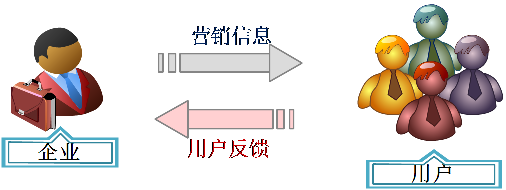
\includegraphics[width=0.65\textwidth]{直效营销示意图}
	\caption{直复营销简化示意图}
	\label{fig:直复营销示意图}
	\end{figure}

近年来,随着信息化和智能化的快速发展,机器学习技术正日益成为直复营销研究的重要方向。最开始,研究人员通过使用监督学习和非监督学习方法中的经典分类模型,以营销决策中的低错误率为学习目标,来解决上述问题。但是,在营销场景中,对不同客户的错误分类给企业所带来的损失是不同的,所以传统的分类算法具有很大的局限性。基于这个不足,研究人员后续提出了很多基于代价敏感(Cost-sensitive)的学习方法,这些方法将不同样本的错误分类赋予不同的惩罚代价,因而当应用于直复营销场景时,可以取得比传统分类算法更好的效果。

但是,在使用上述基于监督学习和非监督学习的方法时,只能最大化单次决策的即时收益,即前一个决策和后一个决策之间是独立的。而在像直复营销这类应用场景中,随着时间的推移需要不断地做出决策,属于序贯决策问题,所以,当营销人员在进行营销决策时,不仅需要考虑到单次营销的成本和收益,还要考虑到随着时间的推移,该次营销对后续营销结果可能产生的影响。比如:在某一次的营销活动中,企业从某个客户那么所得到的预期收益可能会大于营销成本(即利润为负),但是,这次的营销也可能会使得该客户在之后的营销活动中产生更多的消费(即企业获得更多的收益)。所以,在某些时刻,为了让客户在连续的营销活动中能产生更多的利润,营销人员可能要牺牲短期的利润,以达到最大化客户生命周期价值的目的。而基于监督学习或者非监督学习的算法很难实现这一点。

强化学习(Reinforcement Learning, RL)主要用于解决序贯决策问题,它是机器学习的重要组成部分,其学习过程如图$\ref{fig:强化学习过程}$所示:通过智能体(Agent)不断地与环境(environment)进行交互,并从环境反馈的延迟奖赏中学习状态与行为之间的映射关系,以使得可以达到累积奖赏最大化\citep{2016面向强化学习的模型学习算法研究}。从以上交互过程中,可以发现:强化学习在学习过程中考虑到了延迟回报,并且只关心当前采取什么行为可以使整个任务序列达到累积奖赏最大化,因此,强化学习算法可以很好地解决直复营销场景中营销决策点间的相互影响问题,进而实现最大化客户生命周期价值的目标,这也是本文选择使用强化学习技术解决直复营销问题的出发点。特别地,本文只关注基于值函数的强化学习方法。

\begin{figure}[htbp]
\centering
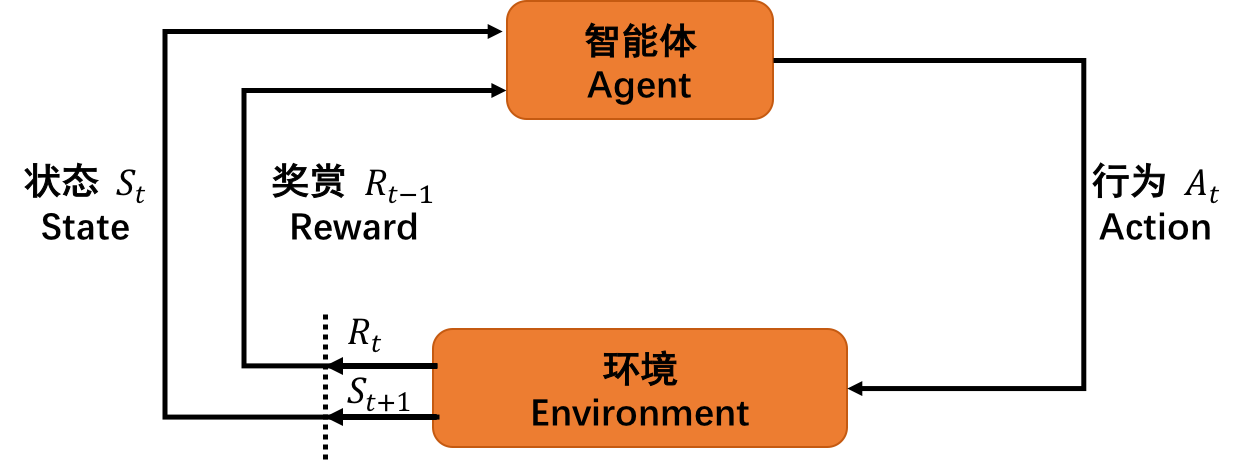
\includegraphics[width=0.8\textwidth]{强化学习过程_}
\caption{强化学习的交互过程}
\label{fig:强化学习过程}
\end{figure}

强化学习是从控制学、心理学、统计学和运筹学等重多学科交叉发展而来的。在1980年到2000年之间,经过众多学者的不懈努力,强化学习的理论研究取得了重大进展,随后被越来越多地用于工业控制、作业调度和机器学习等领域。比如,Macek等人将强化学习技术应用于机器人躲避障碍物\citep{macek2002reinforcement},Tesaruo等人结合神经网络将强化学习应用于西洋双陆棋中\citep{tesauro2006hybrid}。2016年和2017年,DeepMind团队利用深度强化学习(Deep Reinforcement Learning, DRL)技术研发的智能围棋程序AlphaGo大胜世界冠军李世石和柯洁,并引发了研究强化学习的热潮。

虽然强化学习在一些的实际应用中已经取得了重大进展,但是由于强化学习算法理论的复杂性,加之不同应用场景的特殊性,使得强化学习在实际应用中仍然面临着许多困难。在直复营销场景中,虽然近年来已经有学者开始使用强化学习技术来解决直复营销的决策问题,但是以下问题仍然没有得到有效的解决:

(a)在不定期直复营销场景中,因为营销决策点间的时间间隔是不固定的,所以这就会改变回报的计算方式,从而给奖赏带来了一定的噪声影响,进而会影响值函数的学习和优化。

(b)在实际应用中,随着数据量的提升,传统强化学习方法容易出现训练速度慢、学习效率不高的问题。

(c)在直复营销场景中,因为客户的状态存在部分可观测(Partial Observability)问题,所以为了更好地定义客户的状态以进行更高效的策略学习,在实际应用中常常需要借助大量的专家领域知识。

本文在基于值函数的强化学习方法中对以上三个问题进行研究,并给出了相应问题的解决方案。特别地,本文将前两个问题建立在不定期直复营销场景中进行分析,而为了进行更有针对性的研究,将第三个问题独立出来并放在定期直复营销场景中进行分析。

\section{研究现状}
本节首先对直复营销问题的研究现状进行介绍,主要包括传统的分类算法、基于代价敏感的学习算法以及基于强化学习的算法。另外,因为本文的研究是基于强化学习算法的,所以在本节的第二部分也针对强化学习的研究现状进行了介绍。

\subsection{直复营销的研究现状}
在机器学习领域,国内外关于直复营销策略的算法研究,可以概括为以下三个方向。

\paragraph{基于传统的分类算法}

在文献\citep{alam2012actionable, mitik2017data, wong2005mining, coussement2015improving}中作者分别使用了传统的逻辑回归、支持向量机、线性二次判别分析、K近邻、朴素贝叶斯、神经网络以及决策树等算法,利用客户的个人资料和历史营销反馈数据,对客户的响应模型进行建模,研究各类经典分类算法在直复营销中的应用效果,并从模型的策略效果和策略的可解释性等方面给出了权衡意见。尽管这些算法在实际应用中明显优于使用人工经验营销决策的方法,但是,这类算法在学习的时候假设误分类的代价是相同的,而在实际的直复营销应用中,对不同客户的错误营销决策给企业所带来的损失是不同的,所以在营销中使用传统的分类算法必然会存在很大的局限性。

\paragraph{基于代价敏感的学习算法}
针对以上传统经典分类算法在实际应用中存在的不足,众多学者通过引入代价敏感因子进行改进,提出了基于代价敏感的学习算法。在文献\citep{bahnsen2015example}中,Bahnsen等人将误分类代价加入到决策树的构建中,提出了最小代价决策树,并将其应用在了信用卡欺诈检测,信用评分和直接营销场景中,取得了比传统分类算法更好的效果。在文献\citep{cui2012cost}中,Cui等人利用贝叶斯网络自身拥有的先验概率,计算出目标对象属于每个类的概率,然后再直接使用经验风险公式对其进行代价敏感分类,用于解决直邮营销场景下客户的决策分类问题。这些基于代价敏感的学习算法虽然考虑到了误分类的不同代价问题,但是,在进行决策的时候每个决策点都是独立的,只能输出使得当前即时收益最大的策略,因此无法捕捉到直复营销序列中不同决策点间的相互影响,进而也无法达到长期收益最大化目标。有关代价敏感算法的应用研究还有\citep{migueis2017predicting,zakaryazad2016profit,hu2015cost}。另外,通过预测客户在不同状态下所产生利润的回归方法也存在上述的问题。

\paragraph{基于强化学习的算法}
因为强化学习算法在学习过程中考虑到了序列之间的延迟影响,并且以最大化累积奖赏作为学习目标,因此可以很好地解决直复营销场景中不同营销点之间的相互影响问题,进而可以达到最大化客户生命周期价值的目的。近年来,已经开始有学者尝试使用强化学习技术来解决营销中的相关问题。

为了解决监督学习和非监督学习算法独立决策的问题,Pednault等人首次将强化学习技术用于解决直复营销的问题中,提出了使用批强化学习解决该问题的框架,并且对仿真环境的设计和模型的评估方法都给出了有效的解决方案\citep{pednault2002sequential}。但是,对直复营销场景中的一些特殊问题并没有进行分析和讨论。Kim等人针对直复营销场景中存在的客户流失问题,提出将客户的流失概率作为约束条件引入强化学习算法中,并试图在给定的阈值的情况下对其进行自动控制,实验证明该方法可以得到比传统强化学习算法更好的营销策略\citep{kim2009new}。Boutilier等人针对营销过程中存在的预算约束问题,引入带有预算约束的马尔科夫决策过程(Budgeted Markov Decision Process, BMDP),通过权衡预算分配和期望收益之间的关系得到一个关于预算约束的函数,并证明该函数是一个非递减的凹函数,最后使用强化学习方法求出该问题的解,通过实验证明,该方法可以很好地解决带有预算约束的策略决策问题\citep{boutilier2016budget}。Silver等人提出了一种基于时间差分学习的并行强化学习框架。通过该框架可以并发地实现企业与客户之间的交互,并且通过模拟器分别在非自举(non-bootstrappig)、非在线(non-online)和非序列化(non-sequential)三个方面进行了模型的对比评估,得到了在高并发的序列化问题中,应该考虑使用进行自举、在线学习以及使用序列化的强化学习方法的结论\citep{silver2013concurrent}。但是,以上这些算法都没有考虑到在直复营销场景中,营销决策点间的时间间隔不固定给模型的更新带来的偏差影响,也没有有效地解决传统强化学习方法在实际应用中因为数据负载大的导致学习效率不高的问题。

在深度强化学习方面。Tkachenko等人提出使用了深度强化学习方法来解决直复营销中的决策问题,即使用Q-learning的方法训练一个深度神经网络来学习客户的状态和营销行为之间的关系,同时,该文章还使用Recency-Frequency-Monetary(最近的交易时间、交易的频率和交易的金额)指标来描述目标客户的状态,最终实现了客户响应率和客户花费金额两方面的显著提高\citep{tkachenko2015autonomous}。但是该文章仅仅使用深度强化学习来解决线性逼近方法表征能力不足的问题,而没有对神经网络在强化学习中的状态学习方法进行研究。

\subsection{强化学习的研究现状}

\paragraph{发展阶段}
强化学习的总体研究历程,大致可以概括为以下三个阶段。

第一阶段,在1998年以前,这一阶段强化学习的理论框架基本形成,学者们关注最多是基于表格型的学习算法,如:Q-learning\citep{watkins1992q}和Sarsa\citep{rummery1994line}等。
% 代表性的工作是强化学习鼻祖Richard将其专刊装订成书\footnote{http://incompleteideas.net/book/bookdraft2017nov5.pdf},标志着强化学习已经发展成为机器学习的一个重要分支。
% 该书《Reinforcement Learning: An introdcution》是强化学习领域的经典著作,第一次系统而全面的介绍了强化学习的相关理论

第二阶段,在1998年到2013年间,基于策略搜索的强化学习方法得到了深入研究和发展。如GPOMDP算法\citep{baxter2001infinite}、PEGASUS算法\citep{neumann2005reinforcement}以及与值函数方法结合的Actor-Critic算法\citep{konda2000actor}等。

第三阶段,在2013年以后,随着深度神经网络技术的逐渐成熟,出现了深度强化学习算法。代表性的工作是DeepMind团队提出了DQN(Deep Q Network)模型并将其成功应用在雅达利(Atari)游戏和智能围棋程序AlphaGo中\citep{mnih2013playing,mnih2015human}。
% 其中,最具轰动性的事件当属在2016年和2017年,谷歌的利用深度强化学习算法连续两年分别击败了世界围棋冠军李世石和柯洁。
\paragraph{研究热点}

近年来,为了解决强化学习算法在实际应用中容易出现维度灾和收敛不稳定等问题,众多学者主要集中于函数逼近方法进行研究,函数逼近方法可概括为以下三类:

线性函数逼近方法,该方法最早是由Samuel等人于1967年提出的\citep{samuel1959some}。1988年,Sutton等人又将线性函数逼近与带有资格迹的时间差分(Temporal Difference, TD)方法相结合,进而再使用梯度下降求解近似值函数\citep{sutton1988learning},取得了更好的逼近效果,后续相继出现了最小二乘时间差分算法\citep{bradtke1996linear}、离策略(off-policy)函数逼近方法\citep{precup2001off}等。但是,在线性逼近方法中,基函数的类型和参数个数都需要提前确定,因此限制了函数的逼近能力。

% 其中GTD解决了离策略TD学习算法的不稳定问题,且具有较低的时间复杂度\citep{sutton2009convergent}。

非线性函数逼近方法是指使用非线性函数逼近值函数的方法。虽然该方法具有很强的表征能力,但是容易陷入局部最优,且收敛性难以保证。1995年Bertsekas等人利用前向神经网络逼近值函数,取得了相比线性逼近较好的结果,但是往往会出现不收敛的问题\citep{bertsekas1995neuro}。直到DeepMind团队于2013年提出了DQN网络,才使的这一问题得到有效解决。在DQN网络中,通过在训练过程进行经验回放\citep{mnih2013playing}和单独设立目标网络\citep{mnih2015human}的方法,打破了数据之间的关联性,使得神经网络的训练过程收敛且稳定。

% 从此以后,彻底掀起了学术界和工业界研究深度强化学习的热情。2015年DeepMind团队又提出了Double DQN模型,在该模型中为了克服Q-learning本身固有的缺点——过估计(Overestimate),将动作的选择和动作的评估分别使用不同的值函数来实现。除此以外,深度Sarsa、A3C(Asynchronous Advantage Actor-Critic)、DDPG(Deep Deterministic Policy Gradient)等一些列有影响力深度强化学习模型相继被提出。

非参数化函数逼近法,并非没有参数的逼近方法,而是指参数个数和基函数的类型无需提前确定,完全由样本来决定,因此具有更大的灵活性,但是当样本数量很大时,会带来巨大的计算开销。非参数化函数逼近方法主要包括基于高斯过程和
基于核的这两类方法。其中,基于核方法的研究相对较多,如基于核的最小二乘TD算法\citep{xu2005kernel}、基于最小二乘的策略迭代算法\citep{xu2007kernel}等。

\paragraph{发展趋势}
强化学习正在飞速发展,从当前的众多研究工作中可以判断出强化学习的发展具有如下趋势:强化学习与深度学习的结合会更加紧密;强化学习与领域知识的结合更加紧密,特别是在重塑回报函数的方向上;强化学习的理论会更加全面、具体,性能会更加稳定和高效。本文的研究工作正是从前两个方面展开的。

\section{主要研究内容}
因为强化学习算法在学习过程中,考虑到了序列中的延迟影响,并且以累积奖赏最大作为学习和优化目标,因此可以很好地解决传统的监督学习和非监督学习算法在求解直复营销策略时独立决策的问题。基于以上原因,本文选择使用强化学习的方法解决直复营销中的决策问题。首先关注基于线性函数逼近的Q-learning算法,并针对直复营销场景中营销决策点间时间间隔不固定、数据负载大导致训练速度慢这两个问题提出相应的改进方法,然后又针对基于线性函数逼近的Q-learning算法无法很好地解决客户状态的部分可观测问题,研究了基于非线性函数逼近的DQN算法。本文研究内容的结构如图$\ref{fig:研究路线图}$所示,可以具体概括为以下四点:

\begin{figure}[htbp]
\centering
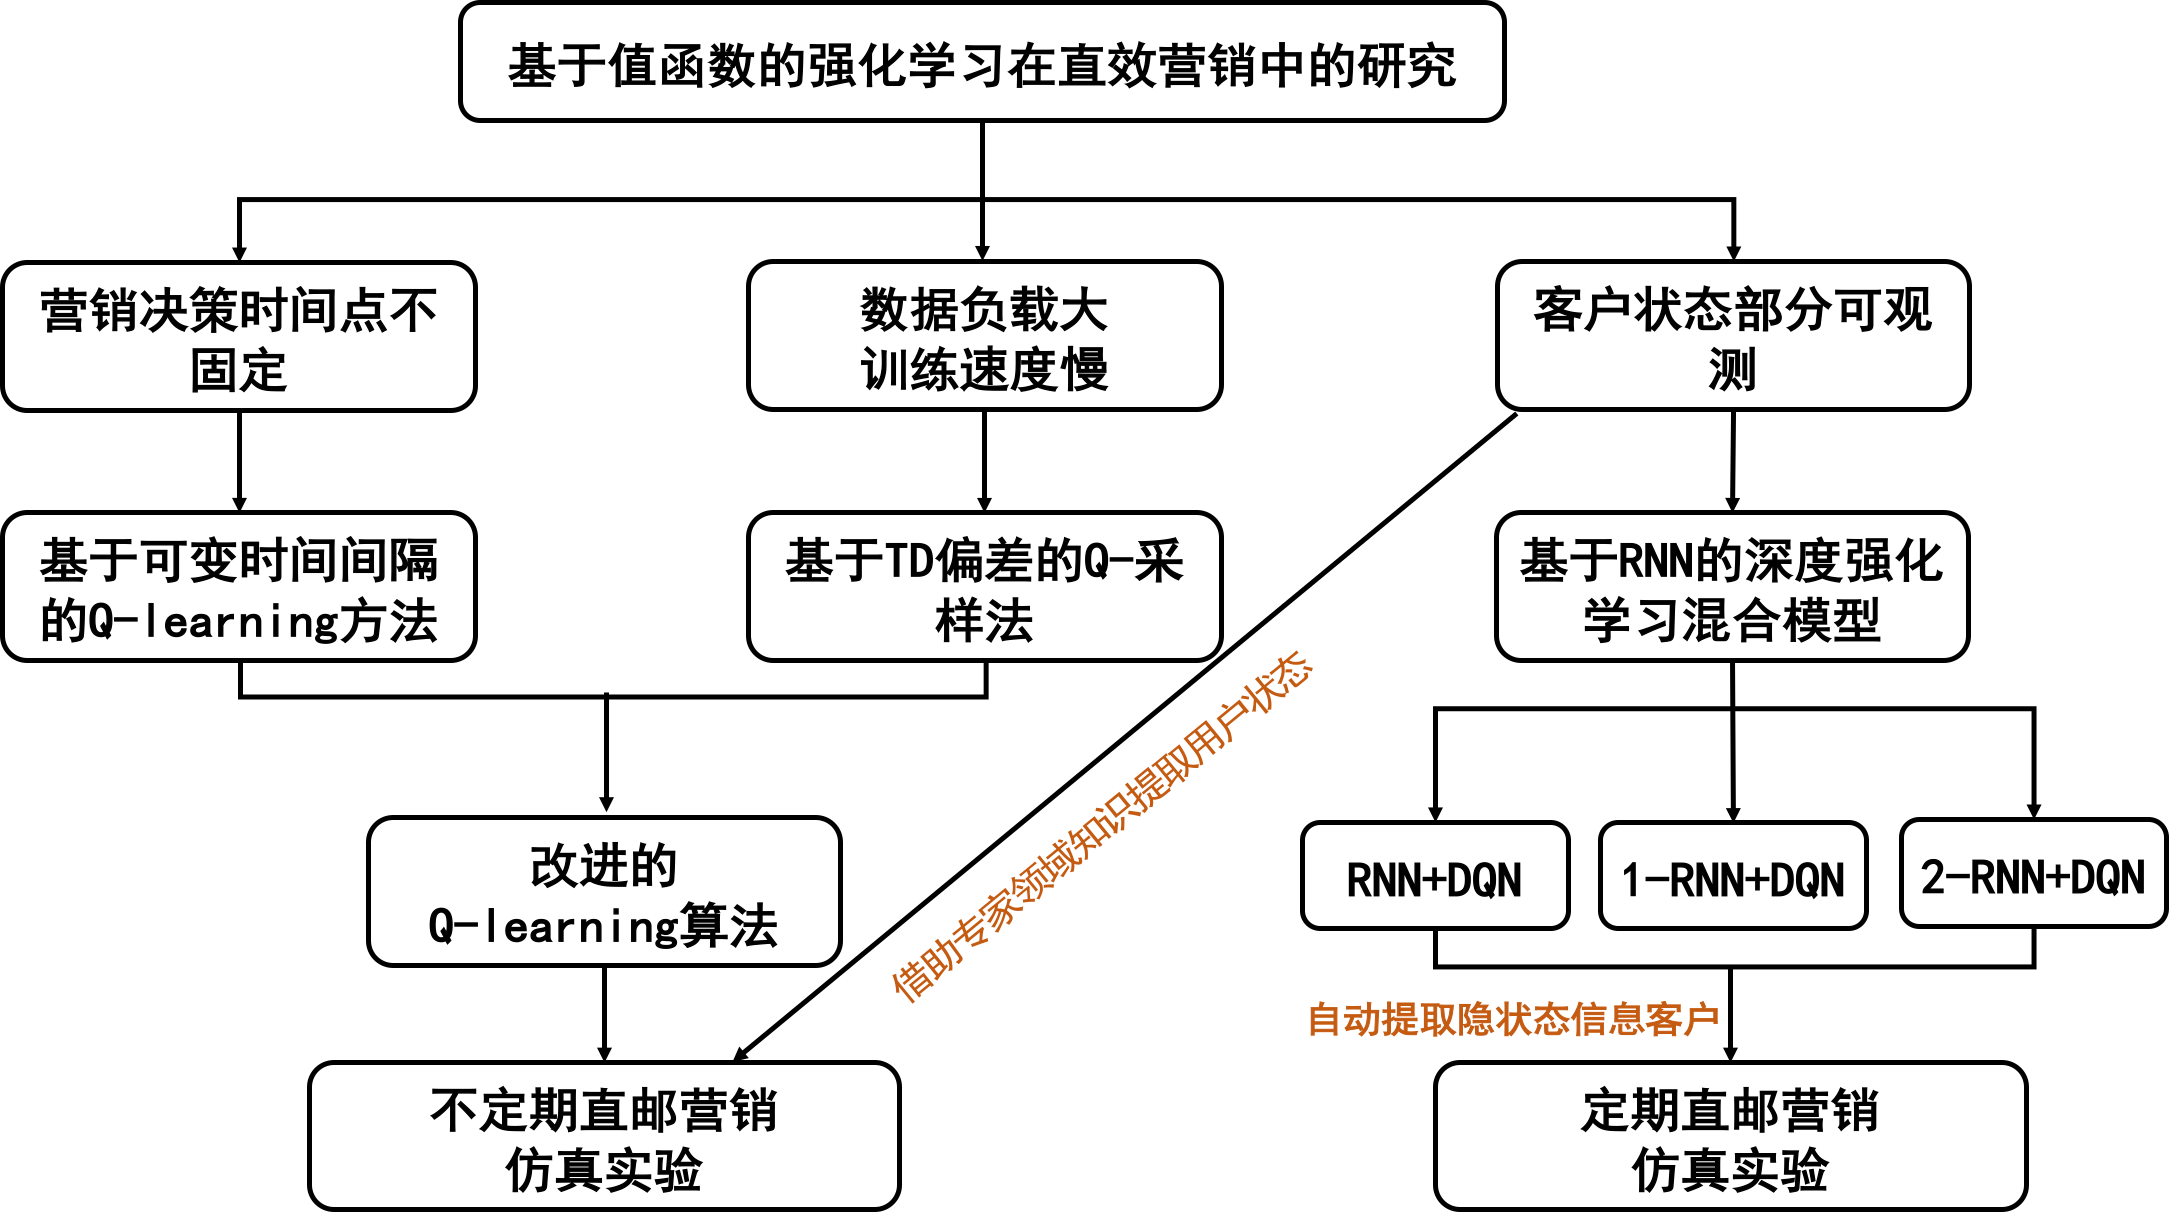
\includegraphics[width=1.0\textwidth]{研究路线图}
\caption{本文研究内容的结构图}
\label{fig:研究路线图}
\end{figure}

(1)针对直复营销场景中营销决策时间间隔不固定和数据规模大导致学习速度慢这两个问题,本文基于传统的Q-learning算法进行研究,并提出了改进的Q-learning算法。具体地,使用均值标准化的方法减少决策点间时间间隔不固定给奖赏信号带来的噪声影响,进而针对Q值函数在迭代过程中因为时间间隔更新不同步而带来的偏差,构建一个标准化因子,并仿照值函数的更新方法进行标准化因子的更新,由此提出Interval-Q算法。接着,针对Interval-Q算法在处理大规模数据时,导致训练速度慢、学习效率不高的问题,本文在Q采样法的基础上,引入TD偏差,提出基于TD偏差的Q采样法。

% 最后,通过仿真实验证明,本文所提的Interval-Q算法在不定期营销中可以取得更高的收益,另外,基于TD偏差的Q采样法,可以在减少采样数量的同时达到更好的学习效果。

(2)利用仿真环境在不定期直复营销场景中对(1)中的改进模型进行评估。
% 针对1)中的两个改进算法使用仿真环境进行评估。
其中,对于本文提出的Interval-Q算法,从策略的长期收益和策略行为的变化情况两个方面进行评估,通过实验证明Interval-Q算法因为考虑到了序列中时间间隔不固定的问题,在不定期直复营销场景中,相比传统的Q-learning算法,可以取得了更高的收益,而且具有更好的成本控制能力。接着,将本文所提出的基于TD偏差的Q采样法从长期收益和采样数两个方面与Q采样法和随机采样法进行比较,验证了所提算法在减少采样数目的同时可以取得更高的收益。需要说明的是,在以上两个实验中,为了解决客户状态的部分可观测问题,进而更好进行值函数的学习,引入了大量的专家知识来提取客户的状态信息。

(3)针对传统强化学习算法无法有效处理直复营销场景中客户状态部分可观测的问题,本文基于深度强化学习DQN模型进行研究,并提出了基于双网络的DQN模型。具体地,首先结合营销场景的时序特点,提出使用基于RNN网络的DQN模型(DQN_RNN)以学习隐状态的方式来解决上述问题。然后,通过分析指出DQN_RNN模型在网络优化过程中不能很好地同时进行隐状态的学习和值函数的逼近,由此提出基于双网络的DQN模型:通过RNN网络从监督数据中学习隐状态的表示方法,再将RNN网络输出的隐状态作为DQN网络的输入状态进行强化学习,通过这种方式可以充分发挥两个网络各自的优势,在提高值函数逼近效果的同时也能更好地学习隐状态。最后,为了取得更好的策略学习效果,又从网络结构和训练方法两个角度进行分析,提出三种改进模型:双网络独立训练模型、双网络一步联合训练模型和双网络两步联合训练模型。

(4)利用仿真环境在定期直复营销场景中对(3)中的改进模型进行评估。首先从模型的长期收益上证明本文所提出的基于双网络的DQN模型相比传统的DQN模型可以产生更多的利润,并且从三种改进模型的学习曲线和长期收益的对比中验证了本文改进方法的有效性。然后,使用不同规模的数据集对模型进行训练,实验结果表明基于双网络的DQN模型不需要利用大批量数据进行训练同样可以产生较好的营销策略。

\section{论文的结构安排}
基于监督学习和非监督学习方法在序贯决策问题中的局限性,本文考虑使用强化学习的方法来处理直复营销场景中的营销决策问题,来最大化客户的生命周期价值,进而达到最大化企业长期收益的目的。具体地,针对直复营销场景中的营销决策点时间间隔不固定和数据负载大导致训练速度慢这两个问题,在传统的Q-learning算法的基础上提出了相应的改进方案。另外,针对在实际应用中,传统的强化学习方法不能很好的处理客户状态的部分可观测问题,提出使用深度强化学习的方法以学习隐状态的方式进行解决,进一步地,为了更好的学习隐状态的表征能力,进而提高值函数的逼近效果,又提出了基于双网络的DQN模型。本文共分为五章,每章的研究内容如下:

第一章: 绪论 \quad 本章首先对直复营销的场景、目标以及本文的研究意义进行介绍,指出传统的监督学习和非监督学习在处理该问题时的局限性,并由此引出了强化学习的方法。接着,分别介绍了直复营销以及强化学习在国内外的研究现状,并结合本文的研究内容进行简要分析,指出目前研究工作中存在的的不足。最后,概括论述了本文的主要研究内容,并对论文的结构安排进行了说明。

第二章: 相关理论概述 \quad 本章首先对强化学习的学习过程进行总体阐述,以便让读者对强化学习有一个总体的认识。接着,对强化学习的理论框架以及三个基本要素(策略、回报和值函数)进行介绍。然后,针对三个基于值函数的经典的强化学习方法进行讲解,以便让读者更好地理解强化学习的思想和求解方法。最后,对值函数的逼近方法进行讨论,阐述各自的优缺点以及适应场景,特别地,对非线性函数逼近方法中DQN模型的改进点进行了详细介绍,为第四章打下理论基础。

第三章: 基于改进的Q-learning算法在不定期直复营销中的研究 \quad 本章首先介绍研究动机,即为什么要使用强化学习的方法进行直复营销策略的研究以及目前Q-learning算法在解决直复营销问题中的不足。接着,针对现实应用中存在的营销决策点间时间间隔不固定和数据负载大导致学习效率低这两个问题,结合Q-learning算法提出对应的解决方法。最后,利用数据集构建不定期直邮营销的仿真环境,对所提出的改进模型进行评估,并对仿真结果进行分析。

第四章: 基于双网络的DQN模型在定期直复营销中的研究 \quad 本章首先介绍研究动机,即为什么使用深度强化学习DQN模型来解决直复营销中的相关问题。接着,介绍DQN模型以及基于RNN的DQN模型(DQN_RNN),然后分析DQN_RNN在优化学习过程中的不足,提出了基于双网络的DQN模型,并从模型的网络结构和训练方法两个方面进行分析,提出三个改进模型:双网络独立训练模型、双网络一步联合训练模型和双网络两步联合训练模型。最后,利用数据集构建定期直邮营销的仿真环境,并对改进的模型进行评估和分析。

第五章: 总结与展望 \quad 本章系统地总结了本文的研究内容,并指出了本文工作存在的不足以及下一步的研究方向。


\cleardoublepage
% \newpage


\chapter{相关理论基础}
强化学习主要用于解决序贯决策问题,而
% 强化学习的目标是求解一个可以使得回报期望最大化的最优策略。
一般的序贯决策问题可以使用马尔科夫决策过程(Markov Decision Process, MDP)的框架来描述,在利用MDP将问题形式化后,又可以使用基于模型的动态规划方法和基于无模型的强化学习方法来解决该问题。特别地,在强化学习中,对于状态和行为空间较大的问题,往往采用值函数逼近的方法进行求解。本章会依次对它们进行简要的介绍。

\section{强化学习过程}
强化学习是机器学习的一个重要分支,它是从控制工程、心理学和运筹学等相关学科发展起来的,最早可以追溯到巴普洛夫的条件反射实验。但是,直到20世纪90年代初强化学习技术才得到重视,并随着强化学习理论的不断发展和完善,目前已经成为人工智能领域的研究热点,广泛应用于机器人控制、无人驾驶和游戏等方面。

强化学习主要用于解决序贯决策问题,所谓决策,是指面对特定的状态,采取什么样的行为,才能使的回报最大化;所谓序贯,是指需要连续不断的做出决策。所以,强化学习属于一种交互式的学习方法,主要是通过智能体(Agent)与环境不断交互,并从环境反馈的奖赏信息中进行学习,目标是最大化未来的累积奖赏。具体交互过程如图$\ref{fig:强化学习过程}$所示:
\begin{figure}[htbp]
\centering
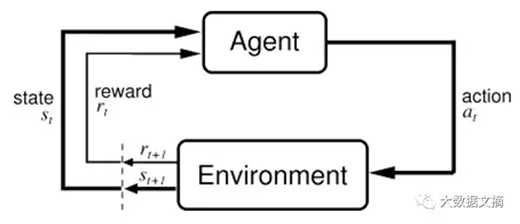
\includegraphics[width=0.6\textwidth]{强化学习过程}
\caption{强化学习的交互过程}
\label{fig:强化学习过程}
\end{figure}

(1)Agent感知当前的环境状态(state);

(2)根据当前的状态和奖赏值(reward),Agent会选择一个行为(action)并执行该行为;

(3)当Agent选择的行为作用于环境时,环境会转移到新的状态,并给出新的奖赏;

(4)Agent根据环境反馈的奖赏,计算回报值(return),并将回报值作为内部更新策略的依据。

 在这一过程中,Agent并不会被告知应该采取哪个行为,而只能经过不断的尝试后,根据得到的环境反馈信息做出判断。Agent选择行为的原则是:所选择的行为应该在以后的学习过程受到环境奖励的概率增大,受到惩罚的概率减小,也就是说,当前采取的行为和最终的目标有关。因为奖励信号是有延迟的,所以Agent有时候宁愿牺牲即时(短期)的奖励以获取更多的长期奖励。因此,试错搜索和延迟回报是强化学习中最重要的两个特征。

 从以上的描述中,可以看出,与监督学习不同,强化学习并不需要多样化的标签数据,而只需要带有回报的交互数据;另外,监督学习是一种反馈学习,即将模型的输出与标签之间所产生的误差信号反馈给模型来指导学习,而在强化学习中,由环境产生的奖赏信号是对所产生行为好坏的一种评价,Agent在行为与评价中获取知识,不断的改进行为方案以适应环境,并不是告诉Agent如何去产生正确的动作。


\section{强化学习的组成要素}
% 介绍马尔科夫决策过程,策略、累计回报、值函数、贝尔曼方程、最优值函数
\paragraph{马尔科夫决策过程}
强化学习可以使用马尔科夫决策过程框架来形式化的描述,MDP通常表示为一个四元组$<S,A,f,h>$,其中:$S$表示有限的状态空间,定义为一个有穷集合$\{ S_1,S_2,\cdots ,S_N \}$,$N$为状态空间的大小。$A$表示有限的行为空间,定义为一个有穷集合$\{ A_1,A_2,\cdots ,A_M \}$,$M$为行为空间的大小。$f$表示状态转移函数,$h$表示奖赏函数。

在马尔科夫决策过程中,考虑在任意的离散时间点$t$时,环境的状态为$S_{t}$,此刻Agent若采取行为$A_t$,就会得到有限的即时奖赏$R_{t}$,并且状态也会相应的转移到下一状态$S_{t+1}$。其中,奖赏$R_{t}$是根据奖赏函数$h$得到的,下一时刻的状态$S_{t+1}$是根据状态转移函数$f$得到的。另外,根据状态转移的情况,可以分为确定性状态转移和随机性状态转移。在确定性状态转移中,状态会转移到确定性的下一状态,而在随机性状态转移中,转移到的下一状态是不确定的,是一个随机变量。

% 又因为马尔科夫决策过程的状态具有马尔科夫性,因此状态转移函数和奖赏函数都仅和当前状态和行为有关,与历史的状态序列和行为序列无关。即:$p(s^{'},r|s,a) = Pr\{S_{t}=s^{'}, R_t=r|S_{t-1}=s, A_{t-1}=a\}$且$\sum_{s^{'}\in S}p(s^{'}|s,a)=1$,$\forall s\in S,\forall a\in A$。
\paragraph{策略和回报}
% \subparagraph{策略}
% 强化学习的目标是从给定的马尔科夫决策过程中,寻找最优的策略。
所谓策略是一个从状态到动作的映射,通常用符号$\pi$表示。
% 指在某一状态下,所采取的动作或所采取动作的概率,。
同样,策略也分为确定性策略和随机性策略,其中确定性策略定义为:$\pi$: $S \to A$ 输出的是一个动作序列,而随机性策略定义为:$\pi$: $S \times A \in [0,1]$ 输出的是该状态下所采取动作的概率:$\pi(s,a)=p[A_{t}=a|S_{t}=s]$。

% \subparagraph{回报}
强化学习的任务是从与环境的不断交互中,学习一个策略$\pi$,使其产生的累积奖赏(cumulative reward)最大化(即回报)。
% 当给定一个策略$\pi$时,如何进行策略的评估呢?此时便用到了累积奖赏的概念。
假设在时刻$t$后接收到的奖赏序列为$\{R_{t+1}, R_{t+2},\cdots\}$,那么采用折扣累积奖赏的方式计算回报可以表示为:
\begin{equation}\label{seq:reward}
G_{t}=\sum_{k=0}^{\infty}\gamma^{k}R_{t+k+1}
\end{equation}

式中,$G_{t}$为回报,$\gamma<1$,为一个常量,称为折扣因子。特别地,在系统与环境的交互过程中,如果任务可以自然地被分为带有终止时间片的片段,则该任务称为情节式(episodes)任务。如果任务无法分解成若干片段,整个任务需要不断的进行下去,则改任务称为连续式(continous)任务。

\paragraph{值函数}
当给定策略$\pi$时,在Agent的学习过程中,考虑评价某一状态的价值,很自然的想法是利用回报来衡量。但是,因为某一状态下的状态序列有很多,所以回报$G_{t}$是个随机变量,不是一个确定的值,无法作为目标函数进行优化。然而,其期望是个确定值,因此可以作为状态值函数的定义:当Agent采取策略$\pi$时,回报服从一个分布,将状态$s$的回报期望值定义为状态$s$的值函数。公式化为:
\begin{equation}
\label{seq2_vs}
v_{\pi}(s)=\mathbb{E}_{\pi}[G_{t}|S_t=s]=\mathbb{E}_{\pi}[\sum_{k=0}^{\infty}\gamma^{k}R_{t+k+1}|S_t=s]
\end{equation}

% Q函数是另一种评估值函数的方法。Watkins指出:。

在某些时候,记录状态行为对的值比只记录状态的值更有用。所以,状态行为值函数定义为在状态$s$下采取行为$a$的回报期望值,公式化为:
\begin{equation}
\label{seq2_qsa}
q_{\pi}(s,a)=\mathbb{E}_{\pi}[G_{t}|S_t=s,A_t=a]
=\mathbb{E}_{\pi}[\sum_{k=0}^{\infty}\gamma^{k}R_{t+k+1}|S_t=s,A_t=a]
\end{equation}

因为上述状态值函数\eqref{seq2_vs}的表达形式在实际应用中很不方便,因此,我们可以经过进一步的推导,得到状态值函数的贝尔曼方程:
\begin{equation}
\label{seq1}
\begin{aligned}
v_{\pi}(s)&=\mathbb{E}_{\pi}[G_{t}|S_t=s]\\
&=\mathbb{E}_{\pi}[R_{t+1}+\gamma G_{t+1}|S_t=s]\\
&=\sum_{a}\pi(a|s)\sum_{s^{'}}\sum_{r}p(s^{'},r|s,a)[r + \gamma\mathbb{E}_{\pi}[G_{t+1}|S_{t+1}=s^{'}]]\\
&=\sum_{a}\pi(a|s)\sum_{s^{'},r}p(s^{'},r|s,a)[r+\gamma v_{\pi}(s^{'})], \forall s \in S
\end{aligned}
\end{equation}
其中,$p(s^{'},r|s,a) = Pr\{S_{t+1}=s^{'}, R_{t+1}=r|S_{t}=s, A_{t}=a\}$,表示在状态$s$时执行行为$a$下,转移到下一个状态$s_{'}$并且得到奖赏$r$的概率。

同样地,也可以得到状态行为值函数的贝尔曼方程:
\begin{equation}
\label{seq2}
\begin{aligned}
q_{\pi}(s,a)=\sum_{s^{'},r}p(s^{'},r|s,a)[r+\gamma \sum_{a'}\pi(a'|s') q_{\pi}(s^{'},a^{'})], \forall s \in S, \forall a \in A
\end{aligned}
\end{equation}

计算值函数的目的是为了构建学习算法从数据中学习到最优策略,而每个策略对应着一个状态值函数,那么最优策略自然对应着最优状态值函数。所谓的最优状态值函数$v_{*}(s)$是指所有策略中值最大的值函数,即$v_{*}(s)==\max_{\pi}v_{\pi}(s)$,同样地,最优状态行为值函数$q_{*}(s,a)$为在所有策略中值最大的状态行为值函数,即$q_{*}(s,a)=\max_{\pi}q_{\pi}(s,a)$

因此,我们又可以由式\eqref{seq1}和式\eqref{seq2}进行推导(因为篇幅限制,推导过程略),分别得到最优状态值函数和最优状态行为值函数的贝尔曼最优方程:
\begin{equation}
\begin{aligned}
v_{*}(s)=\max_{a}\sum_{s^{'},r}p(s^{'},r|s,a)[r+\gamma v_{\pi}(s^{'})]
\end{aligned}
\end{equation}
\begin{equation}
\begin{aligned}
q_{*}(s,a)=\sum_{s^{'},r}p(s^{'},r|s,a)[r+\gamma \max_{a'} q_{\pi}(s^{'},a^{'})]
\end{aligned}
\end{equation}

最后,若求出了最优状态行为值函数,最优策略可以通过直接最大化 $q_{*}(s,a)$来决定:
\begin{equation}
\begin{aligned}
\pi_{*}(a|s) = 
    \begin{cases}
        1 & if \ a=\argmax_{a\in A}{q^{*}(s,a)},\\
        0 & otherwise.
    \end{cases}
\end{aligned}
\end{equation}

最后,需要强调的是:从公式\eqref{seq2_vs}和公式\eqref{seq2_qsa}可以看出,值函数是对未来奖赏的一种预测,对于一个状态$s$,如果它的奖赏很低,但并不意味着它的状态值就低,因为如果状态$s$的后续状态产生较高的奖赏,仍然可能得到比较高的状态值,这就是本文将强化学习技术用于求解营销问题,进而获取长期收益最大化的主要原因。但是,确定值函数需要Agent在其整个生命周期内通过一系列的观察,不断的估计才能得到。所以,我们接下来要做的就是如何快速而准确的获取值函数。

\section{强化学习经典算法}
根据是否依赖于环境,强化学习的求解方法可以分为基于模型的动态规划法和模型无关的强化学习算法。在基于模型的动态规划法中,需要提供精确的环境模型,然后根据环境的动态性利用贝尔曼方程迭代的求解值函数,其本质是动态规划(Dynamic Programming, DP)的思想,通过不断迭代直至稳定,得到精确解。模型无关的强化学习算法无需提供环境模型,根据agent与环境的不断交互收集样本,然后直接利用样本求解状态值函数和状态行为值函数。主要包括蒙特卡罗(Monte Carlo, MC)法和时间差分(Temporal Difference, TD)等算法。

\subsection{动态规划法}
动态规划法是指在给定模型的情况下,求解最优策略的方法。主要包括策略迭代和值迭代两种方法。

策略迭代算法包括策略评估和策略改善两个步骤,且两个步骤交替进行。在策略评估中,算法的每次迭代是建立在上一轮策略改善的基础上,对状态空间中的每个状态进行扫描,并利用贝尔曼方程进行更新,经过不断的迭代,值函数最终收敛至不动点。在策略改善中,算法利用上一轮策略评估得到的值函数,以贪心的方式生成一个新的策略。两
个过程不断交替,直至策略收敛至最终策略。特别地,贝尔曼方程$\eqref{seq1}$中状态值函数$v_{\pi}(s)$使用了其后继状态的值函数$v_{\pi}(s^{'})$来表示,这是自举(bootstrapping)的思想。

以行为状态值函数的策略迭代过程为例,:
\begin{displaymath}
\begin{aligned}
\pi_{0}\xrightarrow{E}q_{\pi_0}\xrightarrow{I}\pi_{1}\xrightarrow{E}q_{\pi_1}\xrightarrow{I}\pi_{2}\xrightarrow{E}q_{\pi_2}\xrightarrow{I}\pi_{3}\xrightarrow{E} \cdots \xrightarrow{I}\pi_{*}\xrightarrow{E}q_{\pi_{*}}
\end{aligned}
\end{displaymath}
其中$E$代表策略评估过程,$I$代表策略改善过程。初始时,策略和值函数都是随机的。在策略评估时,针对每一个状态行为值,使用贝尔曼方程$\eqref{seq2}$进行值函数的更新,直到$q_{k+1}$稳定便结束本轮迭代:
\begin{equation}
\begin{aligned}
q_{k+1}(s,a)=\sum_{s^{'},r}p(s^{'},r|s,a)[r+\gamma \sum_{a'}\pi(a^{'}|s^{'}) q_{k}(s^{'},a^{'})]
\end{aligned}
\end{equation}
在策略改善时,对所有的状态,使用贪婪方法求出新的策略:
\begin{equation}
\begin{aligned}
\pi_{k+1}(s)=\argmax_{a}q_{k+1}(s,a)
\end{aligned}
\end{equation}
在收敛到最优策略时,每一轮的策略都好于前一轮的策略。当策略$\pi$稳定时,迭代过程结束,即得到最优值函数$q_{*}(s,a)$和最优策略$\pi_{*}$。

值迭代算法是对策略迭代的简化,也包括策略评估和策略改善两个环节。与策略迭代不同的是,它不需要等到在策略评估值函数完全收敛时才进行下一次的迭代,而是对全部的状态行为空间每进行一次扫描(更新)就进行策略改善,加快了值函数的收敛速度。对每一个状态行为对,值迭代的更新公式如下:
\begin{equation}
\begin{aligned}
q_{k+1}(s,a)=\sum_{s^{'},r}p(s^{'},r|s,a)[r+\gamma \max_{a^{'}} q_{k}(s^{'},a^{'})]
\end{aligned}
\end{equation}
直到$q_{k+1}$稳定,算法结束。此时因为值函数已经收敛,直接对值函数使用贪心方法就可以得到最优策略。

\subsection{蒙特卡洛方法}
在求解强化学习问题时,由于动态规划法需要提供完整的环境模型且计算代价太大,限制了其在实际场景中的应用。当没有环境模型时,我们可以采用蒙特卡罗方法计算值函数,即用经验平均的思想代替随机变量的思想。其中,经验是指按照该策略做了很多次试验,产生很多情节(episode),每一个情节就是一次实验,平均就是指的平均值,按照求解方法不同又可以分为第一次访问(first-visit)蒙特卡罗方法和每次访问(every-visit)蒙特卡罗方法。在与环境的交互过程中,当一个情节结束后,则进行值函数的更新和策略的改善。另外,值函数的更新可采取可递增(Incremental )计算均值的方法,公式为:
\begin{equation}
\begin{aligned}
V_{k+1}(s)=V_{k}(s)+ \alpha(G_{t}-V_{k}(s))
\end{aligned}
\end{equation}
其中,$\alpha$为学习率,$G_{t}$为从状态$s$出发至情节结束所获的的累积折扣奖赏。

在动态规划中,为了保证值函数的收敛,算法会扫描状态空间的每一个状态。而蒙特卡罗方法想要充分评估值函数的前提是保证每个状态都可以被访问到,因此MC采用了探索性初始化(Exploring Start)的方法,即在每一个情节在迭代时,其初始状态都是随机分配的。

\subsection{时间差分方法}
相比于动态规划法,蒙特卡罗法使用了经验平均,虽然摆脱了对模型的依赖,但是不需要等到每个情节结束就可以进行值函数评估和策略更新,所以学习速度慢,学习效率不高。而动态规划因为使用了bootstrapping思想,所以可以在情节未结束时就可以根据未来值函数估计当前的值函数。时间差分法综合了两者的优点,融合了蒙特卡罗的采样方法和动态规划的bootstrapping思想。

所谓时间差分是指对同一事件或变量在连续两个时刻观测的偏差。TD(0)算法是指一步更新,即值函数直接根据下一个时间步进行学习,估计下一个状态的值函数。
假设在状态$S_{t}$时,Agent采取行为$A_{t}$,获得奖赏$R_{t}$的同时状态转移到$S_{t+1}$。因为环境从状态$S_{t}$向$S_{t+1}$以外的其它状态转移的概率为0,设$V(S_{t})$为最优$v_{*}(S_{t})$的估计值,那么状态$S_{t}$的值函数为:
\begin{equation}
\begin{aligned}
V(S_{t})=R_{t+1}+\gamma V(S_{t+1})
\end{aligned}
\end{equation}
时刻$t$的时间差分为:
\begin{equation}\label{shijiachafen}
\begin{aligned}
\delta_{t}=R_{t+1}+\gamma V(S_{t+1})-V(S_{t})
\end{aligned}
\end{equation}
那么,值函数的更新公式为:
\begin{equation}
\begin{aligned}
V(S_{t}) \gets V(S_{t})+\alpha (R_{t+1}+\gamma V(S_{t+1})-V(S_{t}))
\end{aligned}
\end{equation}
式中,$\alpha$为步长参数,控制学习率,$R_{t+1}+\gamma V(S_{t+1})$称为TD目标,$\delta_{t}=R_{t+1}+\gamma V(S_{t+1})-V(S_{t})$为TD偏差。

根据探索策略(行为策略)和评估策略是否为一个策略,可以将强化学习方法分为同策略(on-policy)和异策略(off-policy)两种方法。同样,时间差分方法也包括了同策略的Sarsa方法和异策略的Q-learning方法。在Sarsa方法中,行动策略和评估策略都是$\epsilon-greedy$的方法,对应的算法伪代码如$\ref{algo:algorithm_1}$所示。

\begin{algorithm}[htbp]
\small
\SetAlgoLined
\SetKwRepeat{Repeat}{Repeat}{until} 
% \KwData{this text}
% \KwResult{how to write algorithm with \LaTeX2e }
初始化$Q(s,a)$,$\forall s \in S$,$\forall a \in A$, 给定参数$\alpha$,$\gamma$\;
\Repeat{所有的$Q(s,a)$收敛}{
初始化起始状态$s$\;
根据$\epsilon-greedy$策略在状态$s$下选择行为$a$\;
\Repeat((对每个情节的每一步)){$s$是终止状态}{
	在状态$s$下选择行为$a$,得到奖赏$r$和下一个状态$s^{'}$\;
	在状态$s^{'}$下根据$\epsilon-greedy$策略得到动作$a^{'}$\;
	$Q(s,a) \gets Q(s,a)+\alpha[r+\gamma Q(s^{'},a^{'}) - Q(s,a)]$\;
	$s=s^{'}$,$a=a^{'}$\;
	}
}
输出最终策略:$\pi(s)=\argmax_{a}Q(s,a)$\;
\caption{Sarsa算法}
\label{algo:algorithm_1}
\end{algorithm}

与Sarsa方法不同,在Q-learning中,行为策略采用$\epsilon-greedy$策略,而目标策略采用贪婪策略,故又称为异策略Q-learning算法,其伪代码如$\ref{algo:algorithm_2}$所示。
\begin{algorithm}[htbp]
\small
\SetAlgoLined
\SetKwRepeat{Repeat}{repeat}{until} 
% \SetAlgoRefName{algorithm_2}
初始化$Q(s,a)$,$\forall s \in S$,$\forall a \in A$, 给定参数$\alpha$,$\gamma$\;
\Repeat{所有的$Q(s,a)$收敛}{
初始化起始状态$s$\;
% 根据$\epsilon-greedy$策略在状态$s$下选择行为$a$\;
\Repeat((对每个情节的每一步)){$s$是终止状态}{
	在Q函数中,根据$\epsilon-greedy$策略在状态$s$下选择行为$a$\;
	执行行为$a$后,得到回报$r$和下一状态$s^{'}$\;
	$Q(s,a) \gets Q(s,a)+\alpha[r+\gamma \max_{a} Q(s^{'},a)-Q(s,a)]$\;
	$s=s^{'}$\;
	}
}
输出最终策略:$\pi(s)=\argmax_{a}Q(s,a)$\;
\caption{Qlearning算法}
\label{algo:algorithm_2}
\end{algorithm}

在TD(0)中,更新当前值函数时,只用到了下一步状态值函数。而TD($\lambda$)考虑从未来的多步进行学习,并且采用加权的方法融合这多步的估计值,$\lambda \in [0,1]$决定了向未来观察的时间步长度。即
\begin{equation}
\begin{aligned}
V(S_{t} )\gets V(S_{t})+\alpha (G^{(\lambda)}_{t}-V(S_{t}))
\end{aligned}
\end{equation}
其中,
\begin{displaymath}
\begin{aligned}
G^{(\lambda)}_{t}=(1-\lambda) \sum_{n=1}^{\infty} \lambda^{n-1} G^{(n)}_{t}\\
\end{aligned}
\end{displaymath}
\begin{displaymath}
\begin{aligned}
G^{(n)}_{t}=R_{t+1}+\gamma R_{t+1}+ \cdots +\gamma^{n-1} R_{t+n}+\gamma^{n} V(S_{t+n})
\end{aligned}
\end{displaymath}

这就是TD($\lambda$)的前向视角表达形式,但是,这种方式需要等到整个实验结束才能计算。后向视角利用增量式的更新方式,不需要等到实验结束就可以更新当前状态的值函数,并且引入了资格迹$Z_{t}(s)$的概念,资格迹记录了最近被访问过的状态,也就是说,最近且最频繁被访问到的状态会被赋予最大的“资格”。更新方式为:

(1)首先,计算当前状态的TD偏差:$\delta_{t}=R_{t+1}+\gamma V(S_{t+1})-V(S_{t})$

(2)其次,更新资格迹:$Z_{t}(s) = 
    \begin{cases}
        \gamma \lambda Z_{t-1} & if s \neq s_{t},\\
        \gamma \lambda Z_{t-1}+1 & if s = s_{t}.
    \end{cases}$

(3)最后,对状态空间中的每个状态$s$,更新值函数:$V(s) \gets V(s)+\alpha \delta_{t} Z_{t}(s)$

综上,后向视角的时间差分方法不仅不需要环境模型,而且利用了增量在线的机制,实现方式简单有效,同时也保证了策略的实时性,被认为是强化学习中最核心的算法。

\section{值函数逼近方法}
至此,我们可以归纳出基于值函数的强化学习的基本步骤是:先评估值函数,然后再利用值函数改善当前的策略。其中,值函数的评估是关键。

在之前所介绍的强化学习方法中,值函数其实是一个表格,其索引是状态或者状态行为对,值迭代更新实际上就是这张表格的迭代更新,因此,这种强化学习称为表格型强化学习,它有一个前提条件:状态空间和行为空间都是离散的,并且状态空间和行为空间不能太大。然而,现实中的很多问题都具有很大的状态(行为)空间,甚至是连续的状态(行为)空间,比如围棋有 $10^{170}$  个状态空间,控制直升机飞行需要的是一个连续的状态空间。在这种情况下,需要我们利用函数逼近的方法表示值函数。从数学的角度来看,函数逼近方法可以分为参数化函数逼近和非参数化函数逼近,其中参数化函数逼近又分为线性参数逼近和非线性参数逼近。

\subsection{参数化函数逼近}
参数化函数逼近是从参数空间到值函数空间的映射,函数的形式和参数的个数事先由先验知识预设,而且参数是通过与目标函数有关样本数据来调整的。对于状态(状态行为)值函数可以由一组参数$\bm{\theta}\in \mathbb{R}^{n} $ 来近似,即:
\begin{equation}
\label{seq_2_3_2}
\begin{aligned}
&\hat{v}(s;\bm{\theta})\approx v_{\pi}(s)\\
&\hat{q}(s,a;\bm{\theta})\approx q_{\pi}(s,a)
\end{aligned}
\end{equation}

我们可以发现,在近似的状态值函数$\hat{v}(s;\bm{\theta})$中,针对每个状态,不再存储其状态值,而是只存储一组参数。把从已知的状态中到的值函数,推广至那些未碰及的状态中,这对于拥有大规模的状态空间来说,相当于对其状态空间进行了压缩。由于 $\bm{\theta}\in \mathbb{R}^{n}$,因此所需的存储开销为$O(n)$,当状态空间规模较大且均为离散时,$n$远远小于为每个状态存储值的开销$|S|$。

以状态值函数为例,我们可以得到目标函数为:
\begin{equation}
\label{seq:fun_approxi_obj}
\begin{aligned}
\argmin_{\bm{\theta}}(v_{\pi}(s)-\hat{v}(s;\bm{\theta}))^2
\end{aligned}
\end{equation}

即通过寻找参数向量$\bm{\theta}$,最小化近似函数$\hat{v}(s;\bm{\theta})$与真实函数$v_{\pi}(s)$的均方差。

值函数更新可以分为增量式学习方法和批学习方法。其中,随机梯度下降法是最常用的增量式学习方法。

由公式$\eqref{seq:fun_approxi_obj}$,我们可以得到参数的随机梯度更新公式为:
\begin{equation}
\begin{aligned}
\bm{\theta} \gets \bm{\theta}+\alpha[v_{\pi}(s)-\hat{v}(S_{t};\bm{\theta})]\triangledown_{\theta} \hat{v}(S_{t};\bm{\theta})
\end{aligned}
\end{equation}

进而,得到值函数的更新如下:
\begin{equation}
\label{seq:gradient}
\begin{aligned}
\triangle \bm{\theta} = \alpha (v_{\pi}(s)-\hat{v}(s;\bm{\theta})) \triangledown_{\theta} \hat{v}(s;\bm
{\theta})
\end{aligned}
\end{equation}

然而,公式$\eqref{seq:gradient}$并不能直接用于强化学习中,因为公式里有一个真实价值函数$v_{\pi}(s)$,或者是一个具体的数值,而强化学习没有监督数据。

从表格型值函数的更新过程中,我们可以看出无论是蒙特卡罗方法还是时间差分方法,都是朝着一个目标值更新的,这个目标值在蒙特卡罗方法中是$G_{t}$,在时间差分方法中是$R_{t+1}+\gamma Q(S_{t+1},A_{t+1})$,在$TD(\lambda)$中是$G^{\lambda}_{t}$。所以,如果将表格型值函数的更新过程推广至值函数逼近过程,那么,逼近值函数$\hat{v}(s;\bm{\theta})$的过程实际上可以看作是一个监督学习的过程,其数据和标签对为$<S_{t}, v_{\pi}(S_{t})>$,其中$v_{\pi}(S_{t})$等价于蒙特卡罗方法中的$G_{t}$,时间差分方法中的$R_{t+1}+\gamma Q(S_{t+1},A_{t+1})$,以及$TD(\lambda)$中是$G^{\lambda}_{t}$。因此,只要将公式$\eqref{seq:gradient}$总的$v_{\pi}(S_{t})$做相应替换就可以进行求解了。

在增量式学习方法学习方法中,每次更新模型需要与环境交互,数据使用一次即抛弃,导致样本使用效率不高。而所谓批方法是从给定一段时期的经验中抽取数据集:$D={<S_{1},v^{\pi}_{1}>,<S_{2},v^{\pi}_{2}>,\cdots,<S_{T},v^{\pi}_{T}>}$中,找到最好的拟合函数$\hat{v}(s;\bm{\theta})$,使的$LS(\bm{\theta})=\sum_{t=1}^{T}(v^{\pi}_{t}-\hat{v}^{\pi}_{t}(S_{t},\bm{\theta}))^2$ 最小,这种方法相当于经历重现(Experience Replay),把一段时期内的经历重新过一遍,更新参数,因此样本的利用效率高。

参数化函数逼近根据所使用逼近函数的不同,可分为参数化线性函数逼近和参数化非线性函数逼近两种。

以状态值函数为例,线性函数逼近可以表示为:
\begin{equation}
\begin{aligned}
\hat{v}(s;\bm{\theta})=\sum^{n}_{i=1}\phi_{i}(s) \bm{\theta}_{i}=\bm{\theta }^{T} \bm{\phi}(s)
\end{aligned}
\end{equation}
其中,$\bm{\theta}=(\bm{\theta}_{1},\cdots,\bm{\theta}_{n}) \in \mathbb{R}$,$\bm{\phi}(s)=(\phi_{1}(s),\cdots,\phi_{n}(s))^{T}$为状态$s$的特征向量,$\phi_{i}(s)$称为特征函数或者称为基函数,常见的基函数有:多项式基函数、傅立叶基函数以及径向基函数等。线性函数逼近不但形式简单、而且可以收敛到全局最优,缺点是表征能力较弱,而且基函数的形式需要事先选定,这也限制了函数的逼近能力。
% 但是正是由于其具备良好的收敛性和理论简单性,在强化学习的参数化方法中得到了充分应用。

在非线性函数逼近中,函数逼近器是关于参数$\bm{\theta}$的非线性函数。到在强化学习的应用场景中,一个状态数据是可能是持续流入的,而且下一个状态通常与前一个状态是高度相关的。因此,我们需要一个适用于非静态、非独立均匀分布的数据的训练方法来得到近似函数。在众多的非线性方法中,神经网络是最为符合的,因为它关于状态可导而且是迭代求解的。

神经网络可以看成是一种参数化基函数的方法。由于基函数的参数是从数据中学习得到的,因此其表示能力大大提升,神经网络的每层都可看成是基于上一层的新的基函数,也就是特征。从这个意义上说,后面一层是前面一层的抽象,这样可以对高维输入降维。

所以,和线性逼近器相比,非线性函数逼近的优点是有很强的表征能力和逼近能力,可以对目标函数以任意精度逼近,但是其收敛性难以保证,容易陷入局部最优,使的学术界对其的研究停滞了很长时间,直到2013年,DeepMind团队提出了一些改进的深度强化学习的训练方法,很大程度上解决了神经网络在强化学习问题中的收敛性问题,并且取得了令人振奋的实验表现,引发了针对此问题的新的研究热潮。具体细节可以参见本文第三章关于DQN的介绍。

\subsection{非参数化函数逼近}
在参数化函数逼近过程中,基函数的形式和参数的个数都需要提前设定,并且值函数的逼近效果很大程度上受到人为的经验的影响。而在非参数化函数逼近中,参数的个数以及基函数的形式并不是固定的,而是由样本决定,具有很高的灵活性。非参数化函数逼近方法包括基于核函数的方法和基于高斯过程的方法。因为本文第四章是使用的基于核函数的非参数化函数逼近的方法,所以此处仅对基于核的非参数函数逼近进行介绍。

基于核函数逼近模型可以表示为
\begin{equation}
\begin{aligned}
&\hat{q}(s,a;\bm{\theta})=\sum^{n}_{i=1}\bm{k}((s,a),(s_{i},a_{i}))\bm{\theta}_{i}\\
&\hat{v}(s;\bm{\theta})=\sum^{n}_{i=1}\bm{k}((s),(s_{i}))\bm{\theta}_{i}
\end{aligned}
\end{equation}
式中,$\bm{\theta}_{1},\cdots,\bm{\theta}_{n}$为参数向量,$\{(s_{i},a_{i})|i=1,\cdots,n\}$为样本集合,$\bm{k}:S\times A \times S \times A \to \mathbb{R} $为核函数。其中,常用的核函数有线性核函数、多项式核函数、径向基核函数以及Sigmoid核函数等。

利用核函数法逼近值函数的关键是能够将问题构造成一个带有核函数的优化问题。非参数化函数学习过程中完全依赖于样本,虽然带来一定的逼近灵活性,但是收敛性难以得到保证。

\section{本章小结}
 本章主要介绍了强化学习的相关理论基础知识。首先,对强化学习的整体交互过程进行简单介绍,让读者可以对强化学习有一个直观的认识和体会;接着,介绍了强化学习的框架马尔科夫决策过程以及强化学习的三个要素:策略、回报和值函数;然后,介绍了强化学习基于模型和模型无关的三种求解方法;最后,针对大规模问题,介绍了求解值函数的两种逼近方法:参数化函数逼近以及非参数化函数逼近。为后面章节做了铺垫。

\chapter{基于改进的Q-learning算法在不定期直复营销中的研究}

普通的监督学习方法和非监督学习方法在处理序列化决策的问题时,只能最大化单个独立事件的即时收益,无法顾及序列上不同决策点之间的相互影响,因而不能很好地处理直复营销这种序贯决策问题。而强化学习算法在学习时,因为考虑到了序列中的延迟影响并且以长期收益最大化作为优化目标,十分擅长处理序贯决策问题,所以本章选择使用强化学习的方法对该问题进行研究。首先,使用经典的强化学习算法Q-learning对直复营销场景进行建模,然后针对营销时间间隔不固定会给奖赏信号带来噪声影响这一问题,提出Interval-Q算法。并且,为了提高在大规模数据集下模型的训练效率,在Q采样方法的基础上,引入TD偏差,提出了基于TD偏差的Q采样方法。最后,在不定期直邮营销的仿真环境中进行模型的评估,以此来验证所提方法的有效性。

\section{研究动机}
\subsection{直复营销与序贯决策}
如本文第一章所述,在直复营销场景中的每个营销时刻点,营销人员都需要根据客户的个人信息和其之前的交互历史,做出应该对哪些客户进行营销的决策。而监督学习和非监督学习方法在求解该问题时,都仅仅只能考虑到最大化单个独立事件的即时收益,并不能保证在一段时间上的长期收益最大化,这与直复营销所追求的最终目标不符。
% 解决这个问题常用的算法有传统的分类算法和基于代价敏感的学习算法,然而这些算法在决策时

直复营销是一个序贯决策过程,即随着时间的推移,营销人员需要不断地做出营销决策,通常以长期收益最大化作为营销效果的评价指标。因此,在制定营销决策的时候,营销人员不仅需要考虑到每个决策行为的成本和其(即时)收益之间的关系,而且还要考虑到不同决策行为之间的相互影响。

考虑如下情景:在某次制定营销决策的时候,营销人员发现,如果此时对某位客户进行营销的话,其产生的估计收益会大于营销成本(即利润为负),那么营销人员就不会对这位客户进行营销了。然而,营销人员应该意识到,即使该客户在此次的营销活动中不会产生即时利润,但正是因为这一次的营销,可能会增加该客户在后续的营销活动中所产生的利润,甚至该利润值会很大,这样看来,此次对该顾客进行营销就很有必要了。所以,当营销人员进行营销决策时,有时候需要牺牲即时收益以获得长期收益最大化。反之亦然,如果频繁地对某一位高质量用户发送营销信息,则会降低该客户所能产生的期望收益,因为每一位客户在一段时间内消费能力是有限的。

\subsection{强化学习}
因为强化学习在学习过程中考虑到了序列中奖赏信号的延迟影响,并且以累积奖赏最大化作为学习目标。所以通过这种学习方式可以很好地处理直复营销决策中不同营销点之间的相互影响,进而达到长期收益最大化的目标,因此文献\citep{pednault2002sequential,archak2010budget,boutilier2016budget}等提出使用强化学习的思想来解决直复营销中的决策问题。但是,在上述相关工作中,以下问题仍然没有得到有效解决:在不定期直复营销场景中,各个营销点之间的时间间隔是不固定的,所以如果采用强化学习中传统累积奖赏的计算方式,就会给奖赏信号带来一定的噪声,从而影响了值函数的学习。另外,在实际应用中,随着数据规模的不断攀升,值函数的学习速度也会变慢,从而给强化学习在现实应用中带来很大的障碍。

本章针对以上两个问题进行分析,提出了相应的改进方法,以更好地解决直复营销问题。首先,利用马尔科夫决策过程,将直复营销问题建模为一个强化学习问题,并给出Q-learning算法解决该问题的框架;然后,为了解决营销决策点间的时间间隔不固定给奖赏信号带来的噪声影响,提出了Interval-Q算法;最后,为了适应在大批量数据下的学习任务,本文在Q采样的基础上,引入TD偏差,提出一种改进的Q采样方法,以提高值函数的学习效率。

\section{改进的Q-learning算法在直复营销中的建模}
在本节中,首先使用Q-learning算法对直复营销场景进行建模,构建一个可以解决直复营销问题的模型框架。然后,结合不定期直复营销中营销时间间隔不固定的问题,对Q-learning算法中值函数更新方法进行改进。接着,为了解决大规模数据集下模型更新的效率问题,在Q采样方法的基础上,提出了基于TD偏差的Q采样法。

\subsection{直复营销问题的形式化描述}
在本文的第二章中提到,强化学习问题可以使用如下马尔可夫决策过程来进行描述:在任意给定的时间点上,假设环境处于某个状态,当Agent采取一个行为时,它会收到一个有限的奖赏,并且环境会相应的转移到下一个状态。在这一过程中,Agent是以最大化累积奖赏作为行为选择的依据,且该奖赏通常是以累积折扣的形式表示。

同样地,在使用强化学习解决直复营销问题之前,首先要使用马尔科夫决策过程对直复营销问题进行形式化的描述:在某一时刻$t$,客户的状态为$S_{t}$,如果营销人员对其采取了营销行为$A_{t}$,那么该客户的状态会根据一定的转移概率转移到下一状态$S_{t+1}$,并且会产生一定的奖赏信息$R_{t}$。以上这个过程始终贯穿于客户和营销人员的营销交互之中,那么,可以使用$\{<S_{t},A_{t},R_{t}>\}_{t=1}^{\infty}$三元组来表示每一次的营销事件。
其中,客户的状态$S_{t}$可以使用客户在该时刻所具有的特征信息来表示,比如文献\citep{tkachenko2015autonomous}中提到的Recency-Frequency-Monetary(最近交易时间、交易频率和交易金额)等,不同的营销行为$A_{t}$代表企业不同类型的营销方式,客户在反馈中所产生的奖赏信息$R_{t}$是指该客户产生的净利润,也就是说,强化学习在解决直复营销的过程中是通过最大化每个客户的生命周期价值,进而来达到最大化企业长期收益的目的。

在强化学习模型的选择上,Q-learning算法(见算法$\ref{algo:algorithm_2}$)以其原理简单、实现方便的优点,在实际中得到广泛应用。所以,接下来本章将参考文献\citep{,pednault2002sequential}中的基于函数逼近的批强化学习方法,给出Q-learning算法解决直复营销问题的模型框架。

\subsection{基于Q-learning的直复营销模型构建}
在传统的Q-learning算法中,值函数其实是一个表格,其索引是状态或者状态行为对,值迭代更新实际上就是这张表格的迭代更新。所以,在Q-learning算法中存在一个假设是,问题的状态空间和行为空间不能太大。然而,在像直复营销这类复杂的现实问题中,为了合理准确地表示客户的状态信息,需要非常多的特征,其状态空间自然非常大,所以,如果这时依旧使用表格的形式进行值函数的表示并不现实。

如第二章所述,对于状态空间较大的问题可以通过函数逼近的方法进行值函数的估计。在强化学习的各类函数逼近方法中,基于非参数化函数逼近的方法虽然具有很好的表征能力,但是随着数据量的增多其计算量呈指数升高,所以,不适合直复营销这类含有大量训练数据的场景。而在参数化函数逼近方法中,基于非线性的逼近方法在逼近过程中存在着收敛困难的问题。因此,本章考虑使用参数化线性逼近的方法进行值函数的逼近。另外,在参数化线性逼近方法中,基于增量式学习方法在参数的更新过程随机性较大,尽管计算简单,但样本的利用效率不高,而基于批的更新方法尽管计算复杂,但是计算效率较高。所以,本节选择使用基于批更新的线性函数逼近方法。

\paragraph{分块线性函数逼近}
尽管线性逼近方法可以收敛到全局最优解,但是它的表征能力较弱,为了缓解这个问题,本节考虑使用分块逼近的思想以提高值函数的逼近精度:

Q值函数分块逼近模型:考虑具有连续状态空间$\mathcal{S}=\{S_{j}|j \in \mathbb{R}\}$和离散行为空间$\mathcal{A}=\{A_{i}\}_{i=1}^{K}$的强化学习问题,利用逼近模型$\mathcal{M}$对该问题的Q值函数进行建模。$\mathcal{M}=\{M_{i},\cdots,M_{K}\}$,其中$K$为离散行为个数。每个离散行为对一个子模型,子模型之间相互独立,称$\mathcal{M}$为Q值函数分块逼近模型。子模型可以采用任意的结构模型,若$K$个子模型结构相同,则称$\mathcal{M}$为同构分块逼近模型,否则称为异构分块逼近模型。

\begin{algorithm}[htbp]
\small
\SetAlgoLined
\SetKwRepeat{Repeat}{repeat}{until} 
\KwData{折扣因子$\gamma$,最大迭代轮数$P$,多项式次数$M$,原始总样本$D=\{e_{i}|i=1,\cdots,I\}$,其中$e_{i}=\{<S_{i,j}, A_{i,j}, R_{i,j}>|j=1,\cdots,l_{i}\}$,($D$表示样本集合,$e_{i}$表示第$i$个情节,$l_{i}$表示$e_{i}$的长度)}
\KwResult{输出最终的逼近模型:$Q^{(P)}$}

\For{all $e_{i} \in D$}{
	初始化第$i$个情节的数据:$D_{i}^{(0)}=\{<S_{i,j}, A_{i,j}, R_{i,j}>|j=1,\cdots,l_{i}\}$\;
}
整合所有情节的数据,生成总样本集合:$D^{(0)}=\cup_{i=1,\cdots,I} D_{i}^{(0)}$\;
将总样本集合$D^{(0)}$,按照行为标签ID$(A_{i,j}) \in \{1,2,\cdots, K \}$分发到各子模型的样本集合中,并利用分块线性函数更新公式$\eqref{pifangfa}$更新模型:$Q^{(0)}=\{Q_{i}^{(0)}\}_{i=1}^{K}$\;
\For{$p=1$ \KwTo $P$}{
	\For{all $e_{i} \in D$}{
		\For{$j$ \KwTo $l_{i}-1$}{
			计算状态行为值:\;
			$v_{i,j}^{(p)}=Q^{(p-1)}(S_{i,j},A_{i,j}) + \alpha^{(p)} (R_{i,j} + \gamma \max_{a} Q^{(p-1)}(S_{i,j+1},a)-Q^{(p-1)}(S_{i,j},A_{i,j}))$\;
		}
		更新第$i$个情节的样本:$D_{i}^{(p)}=\{<S_{i,j}, A_{i,j}, v_{i,j}^{(p)}>|j=1,\cdots,l_{i}-1\}$\;
	}
	整合所有情节的数据,生成总样本集合。$D^{(p)}=\cup_{i=1,\cdots,I}D_{i}^{(p)}$\;
	将总样本集合$D^{(p)}$,按照行为标签ID$(A_{i,j}) \in \{1,2,\cdots, K \}$分发到各子模型的样本集合中,并利用分块线性函数更新公式$\eqref{pifangfa}$更新模型:$Q^{(p)}=\{Q_{i}^{(p)}\}_{i=1}^{K}$\;
}
\caption{基于Batch Q-learning算法的直复营销模型}
\label{algo:SVR+Q}
\end{algorithm}

基于以上分块逼近的思想,本节利用多项式基函数构建一组同构的分块线性逼近模型,记作:$Q=\{Q_{i}\}_{i=1}^{K}$,其中$Q_{i}=\bm{\theta}_{i}^{T} \bm{\phi}(s)$ ,$\bm{\phi}(s)$为多项式基函数。

假设第$i$个行为的样本集为$D_{i}=\{<S_{i,1},V_{i,1}>, <S_{i,2}, V_{i,2}>, \cdots <S_{i,n_{i}},V_{i,n_{i}}>\}$,其中$n_{i}$为第$i$个行为所对应的样本数量,使用批更新方法就是找到最好的拟合函数$Q_{i}$,使的$LS(\bm{\theta}_{i})=\sum_{t=1}^{n_{i}}(V_{i,t}-Q_{i}(S_{i,t},\bm{\theta}_{i}))$,那么,可用线性最小二乘进行逼近:
\begin{equation}\label{pifangfa}
\begin{aligned}
\Delta \theta_{i} = \alpha_{i} \sum_{t=1}^{n_{i}}[V_{i,t}-\bm{\theta}^{T} \phi(S_{i,t})] \phi(S_{i,t})
\end{aligned}
\end{equation}

\paragraph{模型的更新}
在传统的Q-learning算法中,还存在另一个假设,就是Agent可以与环境进行在线的交互。然而,在直复营销场景中,因为场景的复杂性和多样性,很难构建合理的在线交互环境。为了解决这个问题,通常采用批强化学习\citep{lange2012batch}的方法进行解决,批强化学习是强化学习的一种形式,即Agent采取的行为、环境状态发生的转移都不以在线的方式进行,而是使用代表先前经验的大量静态训练数据进行离线的学习,通过这种方式可以再现现实生活应用中的真实交互情况。其中,训练数据由状态向量、动作值以及奖赏值所组成的三元组来构成的。

结合以上批强化学习方法和分块线性函数逼近模型,可以得到用于解决直复营销问题的Batch Q-learning算法框架,如算法$\ref{algo:SVR+Q}$所示。

在算法$\ref{algo:SVR+Q}$中,按照批强化学习的训练方法,将训练数据集$D$分成$I$个情节(episode),每个情节由一系列事件(event)组成,每个事件包含状态$s$、行为$a$和奖赏$r$。在每条情节数据中,保持了事件原有的出现顺序,以这种方式来重现真实的交互的过程。

在第一轮迭代中,首先初始化每个情节中的数据,整合成总样本集合$D^{(0)}$,然后按照总样本集合中行为标签值的不同划分$K$子样本集合,再利用分块线性逼近模型的更新公式$\eqref{pifangfa}$对奖赏值进行逼近,并作为初始的估计Q值函数。在第二轮及之后的迭代过程中,根据上一次的估计值函数,利用Q值函数的更新公式,更新每个情节中每一个事件的状态行为值。当每一轮训练结束后,就将更新后的样本情节进行整合,形成总样本集合$D^{(p)}$,并按照行为标签值的不同划分$K$个子样本集合,然后再利用分块线性逼近模型的更新公式$\eqref{pifangfa}$进行值函数的更新。当所有轮数迭代完毕后,输出最终的Q值函数。另外,对算法中学习率$\alpha$的选取,通常设置为$\alpha=\frac{1}{K}$,目的是让学习的步伐随着迭代轮数的增加而不断减小。

\subsection{Interval-Q算法}
在传统的强化学习中,假设相邻两个事件之间的时间间隔是固定的,所以,如果在$t=0$时刻后接收到的奖赏序列为$\{R_{0}, R_{1},\cdots\}$,那么采用折扣累积奖赏的方式计算回报可用公式$\eqref{seq:reward_3}$来表示:
\begin{equation}\label{seq:reward_3}
G=\sum_{t=0}^{\infty}\gamma^{t}R_{t}
\end{equation}
式$\eqref{seq:reward_3}$中,$G$为回报,$\gamma<1$,为折扣因子。

但是,在不定期直复营销过程中,相邻两个营销决策点之间的时间间隔是不固定的、是不断变化的,有的间隔时间比较长,有的间隔时间比较短,那么不同时间间隔内所产生的即时奖赏对回报$G$的影响程度自然也是不同的。如图$\ref{fig:2_ad_process_}$所示,序列1是一条时间间隔固定的序列,序列2是一条时间间隔不固定的序列,每条序列下面的第一行表示各事件发生的对应时间点,第二行表示该事件所获得的对应奖赏值,为了方便比较,该例中假设序列1和序列2在对应营销点上获得的奖赏值是相同的。以$t_{2}$时刻为例,序列1和序列2在$t_{2}$时刻虽然都获得了相同的奖赏,但是其时间间隔$t_{2}-t_{1}$是不同的,那么,奖赏值$R_{2}$对$t_{1}$时刻的回报也一定是不同的。而公式$\eqref{seq:reward_3}$在计算时只考虑到了序列上决策点发生的先后顺序,所以如果利用公式$\eqref{seq:reward_3}$来计算回报得到的值却是相同的,因此这就会给回报的计算带来一定的影响。

\begin{figure}[htbp]
\centering
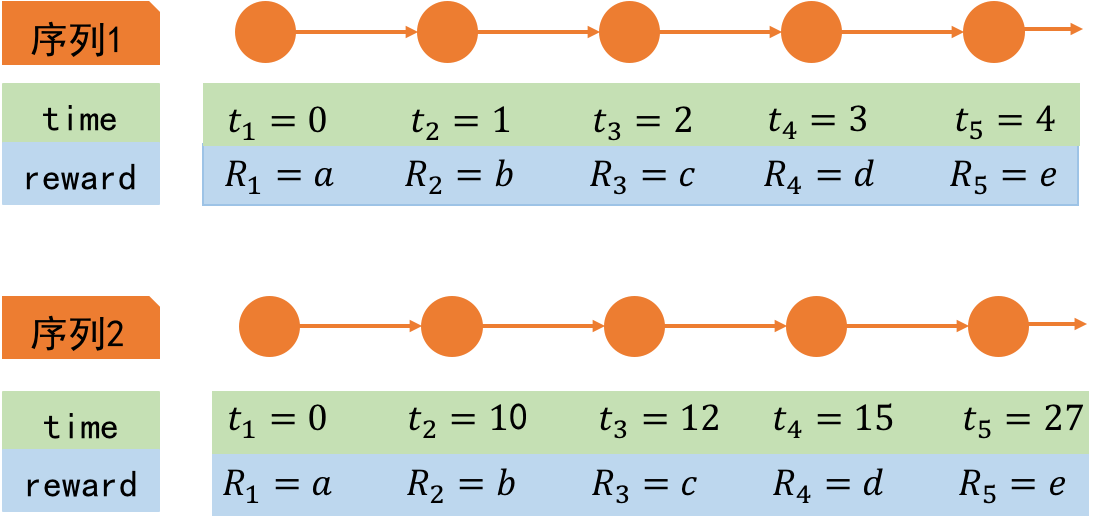
\includegraphics[width=0.8\textwidth]{2_ad_process_}
\caption{固定时间间隔序列和不固定时间间隔序列}
\label{fig:2_ad_process_}
\end{figure}

在有关马尔科夫的理论研究中,将状态逗留时间服从任意分布的决策过程称为半马尔科夫决策过程(Semi-Markov Secision Process, SMDP)\citep{guo2015survey}。SMDP中状态逗留时间不固定和上述不定期直复营场景中营销时间间隔不固定的特点十分相似.但是,不同的是在SMDP中假设时间是连续的,而在直复营销场景中时间是离散的。所以,参考SMDP问题的形式化描述,可以将时间间隔不固定的非定期直复营销问题描述为:

在时间间隔不固定的直复营销决策过程中,首先需要给每次的营销事件标记上时间,假设整个决策过程是从$t_{1}=0$时刻开始的,并且客户的初始状态为$S_{1}$,之后营销人员重复的采取营销行为,便会得到一系列的由状态、行为、奖赏以及时间组成的四元组$\{<S_{i},A_{i},R_{i},t_{i}>\}_{i=1}^{\infty}$,其中$t_{i}$是第$i$个营销事件发生的时间。那么,在计算累积折扣奖赏时,折扣因子就要被定义为关于时间的函数,如式\eqref{seq:r}所示:
\begin{equation}\label{seq:r}
\begin{aligned}
G=\sum_{i=1}^{\infty} \gamma^{t_{i}}R_{i}
\end{aligned}
\end{equation}

下面,考虑将公式\eqref{seq:r}关于累积折扣奖赏的定义结合到Q-learning算法$\ref{algo:SVR+Q}$的更新过程中。如果将第$i$个情节中的第$j$个事件和第$j-1$个事件的时间差记为:$\triangle t_{i,j} = t_{i,j}-t_{i,j-1}$。那么,利用算法$\ref{algo:SVR+Q}$中第5行对奖赏值$R_{i,j}$进行逼近后(作为初始的Q值函数),第10行的状态值的更新公式可表示为\eqref{seq:r1}:
\begin{equation}\label{seq:r1}
\begin{aligned}
v_{i,j}^{(p)}&=Q^{(p-1)}(S_{i,j},A_{i,j}) \\
&+  \alpha^{(p)} (R_{i,j} + \gamma^{\triangle t_{i,j+1}} \max_{a} Q^{(p-1)}(S_{i,j+1},a)-Q^{(p-1)}(S_{i,j},A_{i,j}))\\
% &=(1-\alpha^{(p)})Q^{(p-1)}(S_{i,j},A_{i,j}) + \alpha^{(p)} (R_{i,j} + \gamma^{\triangle t_{i,j+1}} \max_{a} Q^{(p-1)}(S_{i,j+1,},a))\;
\end{aligned}
\end{equation}

\begin{algorithm}[htbp]
\small
\SetAlgoLined
\SetKwRepeat{Repeat}{repeat}{until} 
\KwData{折扣因子$\gamma$,多项式次数$M$,最大迭代轮数$P$,原始样本集合$D=\{e_{i}|i=1,\cdots,I\}$,其中$e_{i}=\{<S_{i,j}, A_{i,j}, R_{i,j}, t_{i,j}>|j=1,\cdots,l_{i}\}$,($D_{i}$表示第$i$个渠道的样本,$e_{i,j}$表示第$i$个渠道第$j$个情节,$l_{i,j}$为$e_{i,j}$的长度)}

\KwResult{输出最终的逼近模型:$Q^{(P)}$}

\For{all $e_{i} \in D$}{
	$\triangle t_{i,1}=1$\;
	\For{$j=2$ \KwTo $l_{i}$}{

		计算时间间隔,$\triangle t_{i,j}=t_{i,j}-t_{i,j-1}$\;
	}
}
\For{all $e_{i} \in D$}{
	\For{$j=1$ \KwTo $l_{i}-1$}{
		初始的标准化因子:$\Gamma^{(0)}_{i,j}=\triangle t_{i,j}$\;
		初始的状态值:$v^{(0)}_{i,j} = R_{i,j}$\;
		将初始的状态值使用标准化因子进行标准化:$D_{i}^{(0)}=\{<S_{i,j}, A_{i,j}, \frac{v^{(0)}_{i,j}}{\Gamma^{(0)}_{i,j}}>|j=1,\cdots,l_{i}\}$\;
	}
}

同算法$\ref{algo:SVR+Q}$中第4行到第5行\;

\For{$p=1$ \KwTo $P$}{
	\For{all $e_{i} \in D$}{
		\For{$j=1$ \KwTo $l_{i}-1$}{
			更新状态行为值\;
			% $v_{i,j}^{(p)}=(1-\alpha^{(p)})Q^{(p-1)}(S_{i,j},A_{i,j}) \cdot \triangle  Z_{i,j}^{(p-1)} 
			% + \alpha^{(p)} (R_{i,j} + \gamma^{\triangle t_{i,j+1}} \max_{a} Q^{(p-1)}(S_{i,j+1,},a) \cdot \triangle  Z_{i,j+1}^{(p-1)} )$\;
			$v_{i,j}^{(p)}=Q^{(p-1)}(S_{i,j},A_{i,j}) \cdot  \Gamma_{i,j}^{(p-1)}
			+  \alpha^{(p)} (R_{i,j} + \gamma^{\triangle t_{i,j+1}} \max_{a} Q^{(p-1)}(S_{i,j+1},a) \cdot \Gamma_{i,j+1}^{(p-1)} -Q^{(p-1)}(S_{i,j},A_{i,j}) \cdot  \Gamma_{i,j}^{(p-1)} )$\;

			更新标准化因子\;
			% $Z^{(p)}_{i,j}=(1-\alpha^{(p)})Z^{(p-1)}_{i,j}+\alpha^{(p)}(\triangle t_{i,j+1} + \gamma^{\triangle t_{i,j+1}} \cdot Z^{(p-1)}_{i,j+1})$\;
			$\Gamma^{(p)}_{i,j}=\Gamma^{(p-1)}_{i,j}+\alpha^{(p)}(\triangle t_{i,j+1} + \gamma^{\triangle t_{i,j+1}} \cdot \Gamma^{(p-1)}_{i,j+1}-\Gamma^{(p-1)}_{i,j})$\;
		}
		更新第$i$个情节的样本:$D_{i}^{(p)}=\{<S_{i,j}, A_{i,j}, \frac{v_{i,j}^{(p)}}{\Gamma^{(p)}_{i,j}}>|j=1,\cdots,l_{i}-1\}$\;
	}
	同算法$\ref{algo:SVR+Q}$中第14行到第15行\;
}
输出最终的Q值函数$Q^{(P)} = Q^{(P)} \cdot \Gamma^{(P)}$\;
\caption{基于Interval-Q算法的直复营销模型}
\label{algo:RBF-SVR-Q-t}
\end{algorithm}

虽然公式\eqref{seq:r1}在更新状态值$v_{i,j}$的时候考虑到了时间间隔不固定的因素($\gamma^{\triangle t_{i,j+1}}$),但是,由于算法$\ref{algo:SVR+Q}$中第5行在利用奖赏值$R_{i,j}$逼近初始的Q值函数的时候,并没有考虑到时间间隔不固定的问题,所以如果按照上述方法逼近Q值函数,并将其应用于公式\eqref{seq:r1}进行状态值的计算更新时会造成很大的偏差。所以,接下来就要寻找一种合适的Q值函数逼近方法。

如上文所述,造成Q值函数逼近不准确的原因是相邻两个决策点间的时间间隔不固定,所以一个自然的想法是利用标准化的思想,将序列中所有的时间间隔都切割成若干个固定单位的时间间隔,然后再进行Q值函数的逼近,进而再按照公式\eqref{seq:r1}更新状态值,就可以缓解因为时间间隔不同而造成的Q值函数逼近不准确的问题。具体的做法是:将时间间隔$\triangle t_{i,j}$内获得的奖赏值进行均值标准化,然后再使用标准化后的值进行Q值函数的逼近。均值标准化的公式如\eqref{seq:r_1}所示:
\begin{equation}\label{seq:r_1}
\begin{aligned}
R_{i, j}^{'}=\frac{R_{i,j}}{t_{i,j}-t_{j-1}}=\frac{R_{i,j}}{\triangle t_{i,j}}
\end{aligned}
\end{equation}

那么,此时算法$\ref{algo:SVR+Q}$中第10行的更新公式就可以按照下式\eqref{seq:r_2}的方式进行更新:
\begin{equation}\label{seq:r_2}
\begin{aligned}
% v_{i,j}^{(p)}=&(1-\alpha^{(p)})Q^{(p-1)}(S_{i,j},A_{i,j}) \cdot \triangle t_{i,j} \\
% &+ \alpha^{(p)} (R_{i,j} + \gamma^{\triangle t_{i,j+1}} \max_{a} Q^{(p-1)}(S_{i,j+1,},a) \cdot \triangle t_{i,j+1})\\
v_{i,j}^{(p)}&=Q^{(p-1)}(S_{i,j},A_{i,j}) \cdot \triangle t_{i,j} \\
&+  \alpha^{(p)} (R_{i,j} + \gamma^{\triangle t_{i,j+1}} \max_{a} Q^{(p-1)}(S_{i,j+1},a) \cdot \triangle t_{i,j+1} -Q^{(p-1)}(S_{i,j},A_{i,j}) \cdot \triangle t_{i,j} )\\
\end{aligned}
\end{equation}

接着,按照算法$\ref{algo:SVR+Q}$中第12行进行情节样本的更新:
\begin{equation}\label{seq:r_3}
\begin{aligned}
D_{i}^{(p)}=\{<S_{i,j}, A_{i,j}, \frac{v_{i,j}^{(p)}}{\triangle t_{i,j}}>|j=1,\cdots,l_{i}-1\}\;
\end{aligned}
\end{equation}

但是,从公式\eqref{seq:r_2}中可以看出,随着迭代轮数的增加,$v_{i,j}$在不断变化,而$\triangle t_{i,j}$是始终不变的,所以,如果一直按照公式\eqref{seq:r_3}中状态值的更新方式($\frac{v_{i,j}^{(p)}}{\triangle t_{i,j}}$)进行样本情节的更新,就会因为这两个值的更新不同步而给值函数的学习带来一定的偏差。因此,本文的想法是,在状态值的更新过程中,应该仿照$v_{i,j}$的更新方式进行$\triangle t_{i,j}$的更新。针对这个问题,本文基于时间间隔构建一个标准化因子$\Gamma_{i,j}$,并仿照$v_{i,j}$的更新方式进行标准化因子的更新,以减少偏差带来的影响。标准化因子的更新方式可表示为式\eqref{seq:r_5}的形式:

\begin{equation}\label{seq:r_5}
\begin{aligned}
% Z^{(p)}_{i,j}=(1-\alpha^{(p)})Z^{(p-1)}_{i,j}+\alpha^{(p)}(\triangle t_{i,j+1} + \gamma^{\triangle t_{i,j+1}} \cdot Z^{(p-1)}_{i,j+1})\\
\Gamma^{(p)}_{i,j}=\Gamma^{(p-1)}_{i,j}+\alpha^{(p)}(\triangle t_{i,j+1} + \gamma^{\triangle t_{i,j+1}} \cdot \Gamma^{(p-1)}_{i,j+1}-\Gamma^{(p-1)}_{i,j})\;
\end{aligned}
\end{equation}

由此,可以得到基于时间间隔不固定的Q-learning算法如$\ref{algo:RBF-SVR-Q-t}$所示,记为Interval-Q。其中,第1行到第6行进行时间间隔的计算,第7行到第13行进行标准化因子以及样本的的初始化,第19行进行状态行为值的更新,第21行进行归一化因子的更新,第23进行情节样本的更新。

\subsection{基于TD偏差的Q采样算法}
在像直复营销这种现实的应用场景中,每天面对的数据量非常大,如果将全部样本都导入模型中进行训练,将必然会加重模型的训练负担消耗很多的训练时间。另外,训练样本中不同样本有着不同的学习效率,有的样本甚至会影响模型的训练效果。所以,针对以上问题,应该采取有效的采样方法来加快模型的训练,以提高值函数的学习效率。

在强化学习中,常用的采样方法有随机采样法\citep{tsitsiklis1994asynchronous}和Q采样法\citep{abe2002empirical}。随机采样法,就是在每次从数据集中取情节的时候(如算法$\ref{algo:RBF-SVR-Q-t}$中,第7行和第16行),并不是取所有的情节,而是随机选取部分的情节。这种随机采样方法虽然可以减少模型的训练和更新时间,但是由于随机性较高,导致采样后的数据质量并不高,因而会影响最后值函数的逼近效果。Q采样法,是在随机采样的基础上利用Q-learning的更新策略提出的,当进行Q值函数进行更新的时候,不是每个情节中所有事件都会被选择用于值函数的更新,而只有那些利用当前的估计Q值函数,可以在下一个状态中取得最佳行为的状态才能被选择。即将算法$\ref{algo:RBF-SVR-Q-t}$的第16到24行替换成如下算法$\ref{algo:SVR+Q_}$的语句:

\begin{algorithm}[htbp]
\small
\SetAlgoLined
\SetKwIF{If}{ElseIf}{Else}{if}{then}{else if}{else}{endif}
从数据集合$D$中随机采样一个样本子集,$B^{(p)}$\;
\For{all $e_{i} \in B^{(p)}$}{
	\For{$j$ \KwTo $l_{i}-1$}{
		\If{$Q^{(p-1)}(S_{i,j+1},A_{i,j+1})=\max_{a}Q^{(p-1)}(S_{i,j+1},a)$}{

			$v_{i,j}^{(p)}=Q^{(p-1)}(S_{i,j},A_{i,j}) \cdot  \Gamma_{i,j}^{(p-1)}
			+  \alpha^{(p)} (R_{i,j} + \gamma^{\triangle t_{i,j+1}} Q^{(p-1)}(S_{i,j+1},A_{i,j+1}) \cdot \Gamma_{i,j+1}^{(p-1)} -Q^{(p-1)}(S_{i,j},A_{i,j}) \cdot  \Gamma_{i,j}^{(p-1)} )$\;

			$\Gamma^{(p)}_{i,j}=\Gamma^{(p-1)}_{i,j}+\alpha^{(p)}(\triangle t_{i,j+1} + \gamma^{\triangle t_{i,j+1}} \cdot \Gamma^{(p-1)}_{i,j+1}-\Gamma^{(p-1)}_{i,j})$\;
		}
		更新第$i$个情节的样本:$D_{i}^{(p)}=D_{i}^{(p)} \cup \{<S_{i,j}, A_{i,j}, \frac{v_{i,j}^{(p)}}{\Gamma^{(p)}_{i,j}}>\}$\;
	}
}
\caption{基于Q采样的算法}
\label{algo:SVR+Q_}
\end{algorithm}

但是,通过Q采样的方法进行采样后的样本仍然很大,而且,即使选择了在下一状态中可以达到最佳行为的当前状态,但是该状态并不一定会有很高的学习效率。考虑在本文第二章中,由公式$\eqref{shijiachafen}$计算出的$t$时刻的时间差分TD:$\delta_{t}$,应用在算法$\ref{algo:SVR+Q_}$的Q值函数中,可表示为式$\eqref{shijiachafenq}$:
\begin{equation}\label{shijiachafenq}
\begin{aligned}
&\delta_{i,j}=R_{i,j} + \gamma^{\triangle t_{i,j+1}} Q^{(p-1)}(S_{i,j+1}, a) \cdot \Gamma_{i,j+1}^{(p-1)}  - Q^{(p-1)}(S_{i,j},A_{i,j}) \cdot \Gamma_{i,j}^{(p-1)} \\
&\text{其中,} a=\argmax_{a} (Q^{(p-1)}(S_{i,j+1},a) \cdot \Gamma_{i,j+1}^{(p-1)})
\end{aligned}
\end{equation}

在式$\eqref{shijiachafenq}$中,$R_{i,j} + \gamma^{\triangle t_{i,j+1}} Q^{(p-1)}(S_{i,j+1}, a) \cdot \Gamma_{i,j+1}^{(p-1)}$称为TD目标,即值函数逼近的目标值。如果TD偏差$\delta_{t}$越大,说明该状态处的值函数$Q^{(p-1)}(S_{i,j},A_{i,j}) \cdot \Gamma_{i,j}^{(p-1)}$与TD目标的差距越大,进一步可以说明Agent的更新量越大,因此在该处的学习效率就越高。所以,TD偏差其实可以作为是评价样本学习效果的一个指标。基于这个想法,在进行Q采样的时候,可以根据TD偏差进行约束。具体地,当使用Q采样算法$\ref{algo:SVR+Q_}$第4行条件进行初步选择后,设定一个固定的阈值$\eta$,然后使用公式$\eqref{shijiachafenq}$再一次进行选择,只选择TD偏差大于$\eta$的样本进行更新。所以,基于这个想法就可以得到基于TD偏差的Q采样法如算法$\ref{algo:SVR+Q_2}$所示。在实际应用中,对于阈值$\eta$的选取可以从训练样本的奖赏均值附近处开始尝试,通过观察采样数和策略学习效果再进一步确定。

\begin{algorithm}[htbp]
\small
\SetAlgoLined
\SetKwIF{If}{ElseIf}{Else}{if}{then}{else if}{else}{endif}
\KwData{增加一个TD偏差阈值$\eta$}
从数据集合$D$中随机采样一个样本子集,$B^{(p)}$\;
\For{all $e_{i} \in B^{(p)}$}{
	\For{$j$ \KwTo $l_{i}-1$}{
			利用公式$\eqref{shijiachafenq}$计算的$\delta_{i,j}$\;
		\If{$Q^{(p-1)}(S_{i,j+1},A_{i,j+1})=\max_{a}Q^{(p-1)}(S_{i,j+1},a)$ $\bm{And}$
			$\delta_{i,j} \geqslant$  $\eta$
		}{
			$v_{i,j}^{(p)}=Q^{(p-1)}(S_{i,j},A_{i,j}) \cdot  \Gamma_{i,j}^{(p-1)}
			+  \alpha^{(p)} (R_{i,j} + \gamma^{\triangle t_{i,j+1}} Q^{(p-1)}(S_{i,j+1},A_{i,j+1}) \cdot \Gamma_{i,j+1}^{(p-1)} -Q^{(p-1)}(S_{i,j},A_{i,j}) \cdot  \Gamma_{i,j}^{(p-1)} )$\;

			$\Gamma^{(p)}_{i,j}=\Gamma^{(p-1)}_{i,j}+\alpha^{(p)}(\triangle t_{i,j+1} + \gamma^{\triangle t_{i,j+1}} \cdot \Gamma^{(p-1)}_{i,j+1}-\Gamma^{(p-1)}_{i,j})$\;
		}
		更新第$i$个情节的样本:$D_{i}^{(p)}=D_{i}^{(p)} \cup \{<S_{i,j}, A_{i,j}, \frac{v_{i,j}^{(p)}}{\Gamma^{(p)}_{i,j}}>\}$\;
	}
}
\caption{基于TD偏差的Q采样算法}
\label{algo:SVR+Q_2}
\end{algorithm}

\section{仿真实验}
本节,将借助直复营销场景中的直邮营销数据进行模型的训练,并通过仿真的方法进行模型的评估。首先,对实验中所使用的数据集进行介绍,并详细说明所选择的客户状态特征;然后,介绍本实验中的仿真环境构建方法和模型效果的评估方法;接着,描述本章实验用到的基准模型以及相关实验设置信息;最后,从模型所产生的长期利润、策略行为的变化情况以及不同采样方法的效果对比等三方面对模型进行评估并对结果进行分析。

\subsection{数据集}
本章的试验数据集选择使用UCI机器学习数据库中关于直邮营销著名的公开数据集KDD-CUP 1998\footnote{https://archive.ics.uci.edu/ml/datasets/KDD+Cup+1998+Data.html}。该数据集有两个用途,一方面,利用数据集中的数据训练模型,以生成最优的营销策略。另一方面,利用该数据集构建基于马尔科夫决策过程的仿真环境,然后利用这个仿真模型进行仿真实验,以评估不同模型所生成的营销策略。

\paragraph{数据集背景}
直邮营销是直复营销中最早的、也是最为经典的营销形式,它通过对目标客户以邮寄的方式达到营销宣传的目的。KDD-CUP 1998数据集是由美国非盈利组织PVA(Paralyzed Veterans of America)收集的,该组织通过直邮的方式向潜在的捐助者发布募捐活动信息以
筹集资金,为有脊髓损伤疾病的美国退伍军人提供医疗资金援助。

该数据集由PVA组织在两年间对95412名捐助者进行募捐营销的历史营销纪录所组成,一共包含22次连续的募捐活动,每个募捐活动之间的时间间隔为0-3个月不等。该数据集中每个捐助者的信息由481维数据组成,这些数据可以概括为以下三个方面的信息:

(a)捐助者的全面人口统计数据,包括家庭和所在地区两个层面的组合数据:比如:捐助者的年龄、收入、性别、家庭信息以及该捐助者所在地区的相关信息等,共计361维。

(b)两年间所进行的22次募捐活动的营销与反馈数据。比如:PVA在每一次的营销活动中是否向该捐助者进行了邮寄营销、进行邮件营销的时间、捐助者是否对PVA的每一次邮件营销产生了捐助反馈、募捐的金额以及募捐的时间,以及在每一次捐助活动时捐助者的RFA( Recency/Frequency/Amount, 距离最后一次募捐的时间/到目前为止募捐的频率/上一次募捐的总额)状态值等信息 ,共计99维,其中募捐的金额从0-1000美元不等。

(c)在最后一次募捐营销结束后每个捐助者的概括信息(Summary Variables)。比如:迄今(最后一次募捐结束后)为止该捐助者捐助的总金额、迄今为止该捐助者捐助的总次数、迄今为止PVA对该捐助者开展邮件营销的总次数以及迄今为止该捐助者所捐助过的最大金额等信息,共计21维。

有关该数据集的其它描述信息可在UCI网站上获得。因为原始数据集中涉及了大量的用户特征,但是在本章实验中只选取了部分特征,所以在本章的后续部分再对所使用的数据特征进行详细介绍。

\begin{table}[htbp]
  \centering
  \caption{捐助者的状态特征}
  \label{tab:obser_donors}
  \begin{tabular}{lll}
    \toprule
      序号 & 特征 & 描述 \\
    \midrule
      1 & age & 捐助者的年龄 \\
      2 &income & 捐助者的收入 \\
      3 &ngiftall & 到目前为止,捐助者捐助的次数 \\
      4 &numprom & 到目前为止,PVA向该捐者发送直邮营销的次数 \\
      5 &frequency & 到目前为止,该捐助者捐助的频率:ngiftall / numprom \\
      6 &ramntall & 到目前为止,捐助的总金额 \\
      7 &recency & 距离上次捐助的时间 \\
      8 &promrecency & 距离上次发送直邮营销的时间\\
      9 &timelag & 第一次直邮营销和第一次捐助的时间\\
      10 &recencyratio & recency / timelag\\
	  11 &promrecratio & promrecency / timelag\\
      12 &nrecproms6 & 之前六个月里,给该捐者者发送直邮营销的次数\\
      13 &nrecgifts6 & 之前六个月里,捐助者捐助的次数\\
      14 &totrecamt6 & 之前六个月里,捐助者捐助的金额之和\\ 
      15 &nrecproms3 & 之前三个月里,给该捐者者发送直邮营销的次数\\
      16 &nrecgifts3 & 之前三个月里,捐助者捐助的次数\\
      17 &totrecamt3 & 之前三个月里,捐助者捐助的金额之和\\            	  
	  % 18 &action & PVA的营销类型,0表示未进行,1表示已进行\\
	  % 19 &money &  捐助的金额\\
    \bottomrule
  \end{tabular}
\end{table}

\paragraph{数据处理与特征选择}
首先,需要确定算法中的数据结构。在算法$\ref{algo:RBF-SVR-Q-t}$中,数据是以情节(episode)的形式存在的,每个情节内又包含一系列有序的事件(event),每个事件是由状态,行为、奖赏和时间所构成的四元组。因此,在KDD-CUP 1998数据集中,可以将每个捐助者的22次营销数据序列看作一个情节,每一次的营销看作情节中的一个事件。那么,每个捐助者就对应一个情节,每个情节里有22个事件,且22个事件是按照真实的营销时间有序排开的。特别地,每个事件里包括该捐助者当时的状态特征,PVA对其采取的营销行为、此次营销捐助的金额以及该营销活动所发生的时间。

为了能够准确地描述捐助者在每一次营销活动中的状态,通常需要借助专家领域知识,选取高效的用户特征。本节主要参考文献\citep{tkachenko2015autonomous, pednault2002sequential}中客户特征的选取方法,从KDD-CUP 1998数据集中提取募捐者的状态特征。具体地,针对每个捐助者的个人基本信息,本章只选择了年龄和收入两个指标,此外,根据数据集中募捐者的历史营销记录,生成了许多临时特征,以更好的捕捉募捐者的近期状态,如表~\ref{tab:obser_donors}所示。从表~\ref{tab:obser_donors}中可以看到,本节使用了一个六个月的历史时间窗口和一个三个月的历史时间窗口来提取捐助者的近期状态特征,所以,数据库中最开始的六个月数据就被用于构建第一个历史窗口信息了,那么,一个情节中的22个事件就只剩下16个左右可以用于模型的训练了。

需要注意的是,在表~\ref{tab:obser_donors}中,捐助者的大部分状态特征都无法从数据集中直接获得,而只能通过遍历数据库进行统计、计算而得到。比如,在数据集中,每个捐助者的numprom字段只有一个值,它表示的意思是最后一次营销(第22次)结束后向该捐助者发送直邮营销的次数 ,那么为了得到之前21次营销活动中该捐助者的numprom值,应该按照营销活动的顺序从后往前进行遍历,每当在数据集中发现PVA对该捐助者进行了邮寄,就进行减一操作。同样,对于ngiftall字段,在数据集中每个捐助者也只有一个值,它表示的意思是最后一次营销结束后该捐助者一共捐助的次数,而为了得到之前21次营销活动中该捐助者的ngiftall值,应该按照营销活动的顺序从后往前进行遍历,每当在营销活动中发现该捐助者进行了捐助就进行减一操作。按照上述方式就可以得到在每次营销活动时捐助者的ngiftall和numprom值了,那么捐助者的frequency也就可以求出来了。同样地,表~\ref{tab:obser_donors}中的其他特征也可以按照这种方式求得。

另外,算法\ref{algo:RBF-SVR-Q-t}中的行为(action)对应PVA的营销类型,0表示未进行直邮营销,1表示已进行直邮营销;算法中的奖赏(reward)信息对应PVA所获得的募捐利润值。

\subsection{仿真环境及评估方法}
因为强化学习算法主要用于解决序贯决策问题,所以评估强化学习模型的好坏需要有稳定的仿真环境。目前,OPENAI\footnote{https://openai.com/}提供了许多游戏的仿真环境开源库,科研人员可以通过其提供的API接口非常方便的调用这些仿真环境,来训练、测试自己的模型,因此,这也是目前大多数强化学习的研究者选择在游戏领域进行研究的一个重要原因。然而,在其它的一些现实应用中,需要研究人员根据数据集自己构建仿真环境。在本节,利用KDD-CUP 1998数据集,按照文献\citep{pednault2002sequential}中提供的方法,通过构建关于募捐者的马尔科夫决策过程模型来搭建仿真环境,进而评价模型输出策略的好坏。

\paragraph{构建MDP模型}
马尔科夫决策过程主要由两个模型组成:第一个模型$P(s,a)$是用来预测捐助者的产生募捐反馈的响应概率,它是一个关于状态$s$和行为$a$的函数。第二个模型$A(s,a)$用来预测如果募捐者对此次募捐邮件产生了响应,会产生多少金额的捐款。在本节的实验中模型$P(s,a)$和$A(s,a)$分别使用随机森林分类模型和随机森林回归模型进行构建。

当有了模型$P(s,a)$和$A(s,a)$就可以使用如下过程来构建马尔科夫决策过程了。(如图$\ref{fig:simulation}$中“仿真环境模块”所示)

(a)给定状态$s$和行为$a$下的即时利润$R(s,a)$可以通过以上这两个模型得到:以$P(s,a)$的概率来掷一枚硬币,并以此来判断捐助者是否会产生反馈。即:出现正面的概率为$P(s,a)$表示捐助者会产生反馈,出现反面的概率为$1-P(s,a)$表示捐助者忽略掉了本次募捐邮件,不会产生任何反馈信息。如果没有出现反馈,那么捐助额为$0$,如果产生了反馈,那么用户的捐助金额为$A(s,a)$。即时利润$R(s,a)$等于捐助额减去邮寄的成本。

(b)状态转移方程也可以使用上述这两个模型通过独立地计算每一维状态特征的变化值而得到。比如:如果PVA采取的行动为1(进行邮寄营销),numprom的值就会加1,否则保持不变;同样的,如果通过上述方式投掷的硬币出现正面朝上,那么ngiftall的值就会加1,否则保持不变;有了这两个值(numprom,ngiftall),那么frequency的值也就可以计算出来了。类似的,其他状态特征也是通过这种方法计算得到的。

\begin{figure}[htbp]
\centering
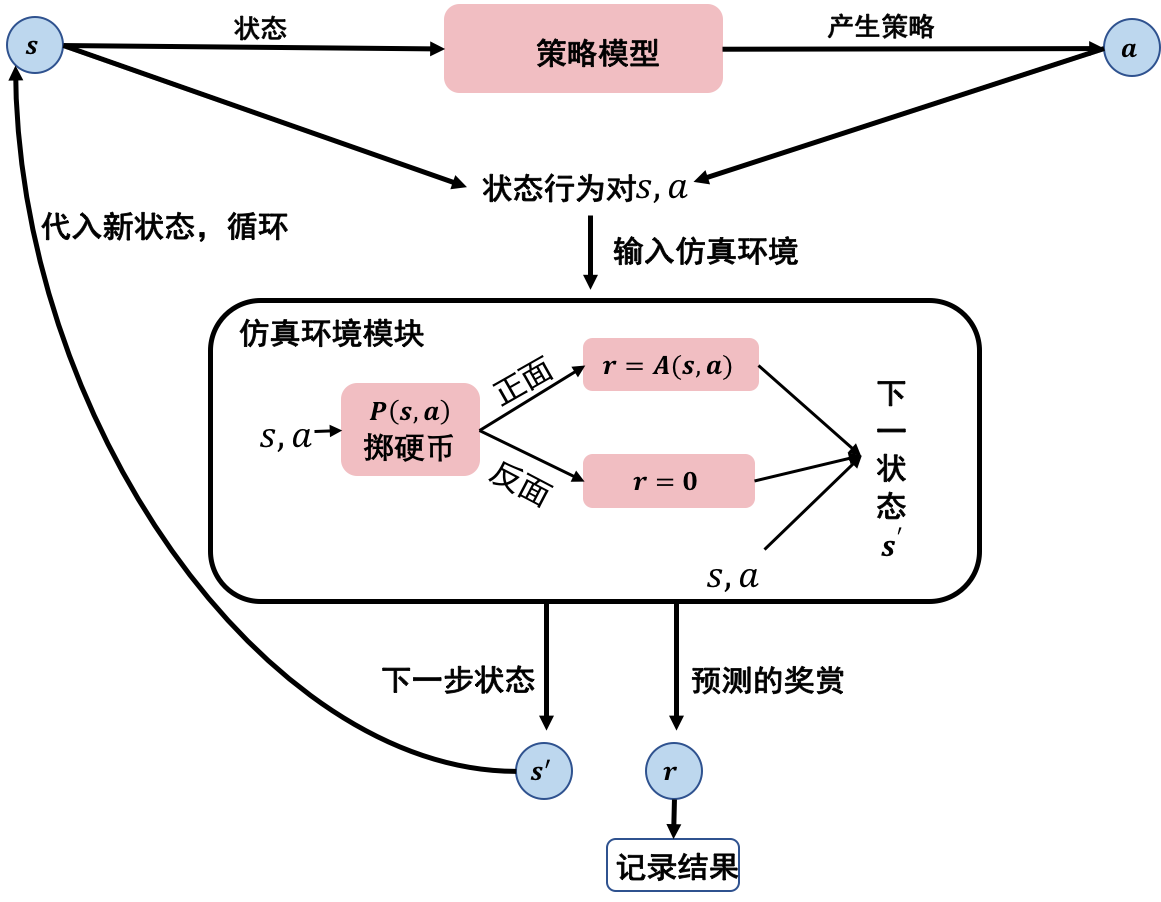
\includegraphics[width=0.8\textwidth]{simulation}
\caption{仿真评估实验流程图}
\label{fig:simulation}
\end{figure}

\paragraph{评估方法}
如图$\ref{fig:simulation}$所示,有了上述基于马尔科夫决策过程的模型和状态转移方程,就可以使用如下的方式来评估实验。

(a)首先,从数据集中随机选择一定数量的捐助者,并设置他们的初始状态$s$。

(b)然后,使用训练好的强化学习模型输出营销策略:对每个捐助者是否应该采取营销行为$a$。

(c)最后,将状态$s$和策略行为$a$代入仿真环境中,使用模型$P(s,a)$和$A(s,a)$,就可以得到预估的即时奖赏$r$以及下一时刻的状态$s^{'}$。记录这些得到信息,然后进入下一次的邮寄决策中。

此后,按照上述的三个步骤,每循环一次就会模拟一次虚拟的直邮营销过程。在本节实验中,重复循环了20次,就得到了20次的虚拟直邮营销数据,通过计算每个模型策略在20次虚拟营销中的长期利润,进而评价模型策略的好坏。

在文献\citep{pednault2002sequential}中作者提出,构建上述仿真环境的前提假设是认为募捐者的交互过程是一个马尔科夫决策过程,但是,在现实中这不一定是合适的。作者认为,像直复营销这种与人类行为有关的场景都过于复杂,使用简单的马尔科夫决策过程是无法较好地捕捉到环境的变化规律的。但是,就像在本章中,通过这种方法设计的仿真环境只是去评估模型所产生的策略的好坏,只是在真实场景应用前的一个评估实验。因此,这种评估方法是可接受的,也是目前强化学习评估实验所普遍采用的方法。

\subsection{基准模型与实验设置}
\paragraph{基准模型}
在本节一共选择四个基准模型来验证上述两个改进的算法,其中Interval-Q算法的对照基准模型包括:多项式回归模型以及Batch Q-learning算法\citep{pednault2002sequential}。基于TD偏差的Q采样算法的基准模型包括:随机采样法和Q采样法。因为随机采样法和Q采样法在本章第二节的内容都有介绍,所以下面只介绍Interval-Q算法的基准模型。

监督模型:多项式回归模型。为了比较监督学习和非监督学习在序列决策问题中的差异,考虑使用监督学习方法作为基准模型。另外,因为在Interval-Q算法中,函数逼近模型采用的是多项式回归模型,所以,为了公平起见,此处仍然选用多项式回归模型作为对照的监督学习模型。在训练模型时,只要将算法$\ref{algo:SVR+Q}$中的$P$设置为0即可,即基于状态$s$和行为$a$来预测即时利润$r$,将学到的模型记为$\hat{R}(s,a)$。当模型训练好后,将募捐者的状态$S_{t}$带入模型$\hat{R}(s,a)$中来估计进行营销时所能获得的即时利润,如果即时利润不为负,则发送营销邮件,否则不发送。

强化学习模型:Batch Q-learning算法。通过此算法来比较引入时间间隔不固定的因素后对模型策略效果所产生的影响。


\paragraph{实验设置}
(a)所有实验运行在Mac Pro机器上,内存16GB,实验语言:Python,机器学习工具包:scikit-learn。

(b)本节试验中,每个模型在相同的参数设置下,分别进行5次试验,每次实验最大迭代轮数$P$为8轮(包括第0轮,其实一共迭代了9轮)。每一轮迭代结束后输出模型所产生的营销策略并按照上述方法使用仿真环境评估该策略,最后取5次实验中每一轮迭代的平均值作为该模型该轮迭代的结果。另外,测试的样本规模大小为5000,并设置他们的初值状态为数据库中对应第7次营销活动时的状态。

(c)在所有的强化学习方法中,衰减因子设为$\gamma=0.9$,通过交叉验证法确定多项式最高次数为5。

% (d)在使用随机森林构建仿真环境时,通过网格搜索法确定以下参数:最大的弱学习器的个数为115个,决策树最大深度为25,叶子节点最少样本数为3,其它参数均选择sklearn的默认值。

\subsection{仿真结果}
下面,本节将从模型策略的长期利润、策略行为的变化情况以及不同采样方法的效果对比等三方面展开对模型的评估与分析。具体地,从模型在20次虚拟营销中所获得的累积总利润、策略行为的变化情况来比较Interval-Q算法、Batch Q-learning算法以及多项式回归算法策略的质量。从模型训练时事件的采样数以及该采样数下所产生的长期利润这两个角度来比较基于TD偏差的Q采样法、Q采样法以及随机采样法的性能。

\paragraph{长期利润}
首先,考察Interval-Q算法,Batch Q-learning算法以及多项式回归模型在20个虚拟营销中的累积总收益,即长期利润。在该实验中,每次实验都随机选取10000个用户的历史营销纪录,也就是10000个情节数据进行训练,每进行完一轮迭代就按照上述方法利用仿真环境进行评估测试,评估模型此时的营销策略在20个虚拟营销中的总利润,并将每一次迭代所产生的结果记录下来。其中,测试集的样本大小为5000。

\begin{table}[htbp]
\centering
\footnotesize
\caption{Interval-Q算法的长期利润(单位:百美元)}
\label{tab:3result1}
\begin{tabular}{|c|ccccccccc|}  
 % \toprule
 \hline
   \diagbox{试验次数}{迭代数} &0 & 1&2 &3 &4 &5 &6 &7 &8\\
% \midrule
\hline

第一次 &5123	&5299	&5557	&5723	&5847	&5854	&5867	&5864	&5868\\
第二次 &5224	&5339	&5666	&5811	&5908	&5911	&5921	&5926	&5920\\
第三次 &5262	&5404	&5602	&5843	&5984	&5981	&5996	&6013	&6015\\
第四次 &5102	&5324	&5569	&5711	&5792	&5888	&5905	&5907	&5917\\
第五次 &5181	&5333	&5602	&5813	&5968	&5971	&5987	&5985	&5987\\
\hline
平均值 &5178	&5340	&5599&5780	&5890	&5921	&5935	&5939&	5941\\
\hline
标准差 &	&17	&17	&18	&33	&22&22	&25	&24\\
% \bottomrule
\hline
\end{tabular}
\end{table}

\begin{table}[htbp]
\centering
\footnotesize
\caption{Batch Q-learning算法的长期利润(单位:百美元)}
\label{tab:3result2}
\begin{tabular}{|c|ccccccccc|}  
 % \toprule
 \hline
  \diagbox{试验次数}{迭代数} & 0 & 1&2 &3 &4 &5 &6 &7 &8\\
% \midrule
\hline
第一次 &5123	&5234&	5586&	5735&	5797&	5814&	5798&	5795&	5801\\
第二次 &5224	&5322&	5659&	5786&	5841&	5883&	5887&	5897&	5870\\
第三次 &5262	&5453&	5655&	5806&	5869&	5927&	5935&	5929&	5936\\
第四次 &5102	&5358&	5578&	5601&	5659&	5679&	5710&	5707&	5713\\
第五次 &5181	&5499&	5698&	5781&	5862&	5918&	5926&	5937&	5936\\
\hline
平均值 &5178	&5373&	5635&	5742	&5806&	5844&	5851&	5853&	5851\\
\hline
标准差 &	&	43	&21	&34	&35	&42	&39	&41&	39\\
% \bottomrule
\hline
\end{tabular}
\end{table}

表~\ref{tab:3result1}和表~\ref{tab:3result2}分别展示了Interval-Q算法、Batch Q-learning算法在这5次试验中的每一轮迭代结束后各模型策略所产生的长期利润值。其中,两个表中第0轮迭代的结果是指多项式回归模型策略的在20个虚拟营销中的总利润,表中标准差的计算方式如式\eqref{seq:shiyan_2}所示。
\begin{equation}\label{seq:shiyan_2}
\begin{aligned}
\sigma = \sqrt{\frac{\sum_{i=1}^{n}(F_{i}-\bar{F})^{2}/n-1}{n}}
\end{aligned}
\end{equation}

在式$\eqref{seq:shiyan_2}$中,$F_{i}$表示在第$i$轮迭代中的总收益,$\bar{F}$表示5次迭代中的平均收益,$n$表示试验的次数,此处为5。

为了方便观察,将表~\ref{tab:3result1}和表~\ref{tab:3result2}中的平均值画在折线图上,如图\ref{fig:e31}所示。从图\ref{fig:e31}中可以看出,Interval-Q算法和Batch Q-learning算法的营销策略在20次虚拟营销中的总利润明显大于多项式回归算法营销策略的总利润,这是因为强化学习算法在求解序贯决策问题时,考虑到了序列中的延迟影响,并且以长期收益最大化作为学习目标,而多项式回归算法在学习时,只考虑了独立事件的即时利润最大化,因此在序贯决策问题时相比强化学习方法有很大的局限性。

另外,从Interval-Q算法和Batch Q-learning算法的迭代过程中可以看出,随着迭代轮数的增长,Interval-Q算法在第3轮迭代后产生的总利润超过了Batch Q-learning算法的总利润,并且在最后一轮迭代时Interval-Q算法产生的长期利润比Batch Q-learning算法的长期利润提高了约1.54\%。这是因为Interval-Q算法在更新时考虑到了营销时间间隔不固定的问题,而Batch Q-learning算法忽视了这种情况,从而会给积累奖赏的计算带来噪声影响,进而会给值函数评估造成偏差,导致学习到的营销策略较差。另外,经计算,Batch Q-learning算法在8轮迭代中标准差的平均值为37大于Interval-Q算法在8轮迭代种的标准差的平均值22,因而说明了在时间间隔不固定的问题中,Interval-Q算法比Batch Q-learning算法输出营销策略时的稳定性更好。至此,可以证明本章的Interval-Q算法在解决时间间隔不固定问题上是有效的。

% 一方面证明强化学习的方法比监督学习的方法在序列化决策问题上会有更好的收益,另一方面期望证明基于可变时间间隔的ntervalQ模型在直复营销场景中比普通batch Q-learning模型有更好的表现。
\begin{figure}[htbp]
\centering
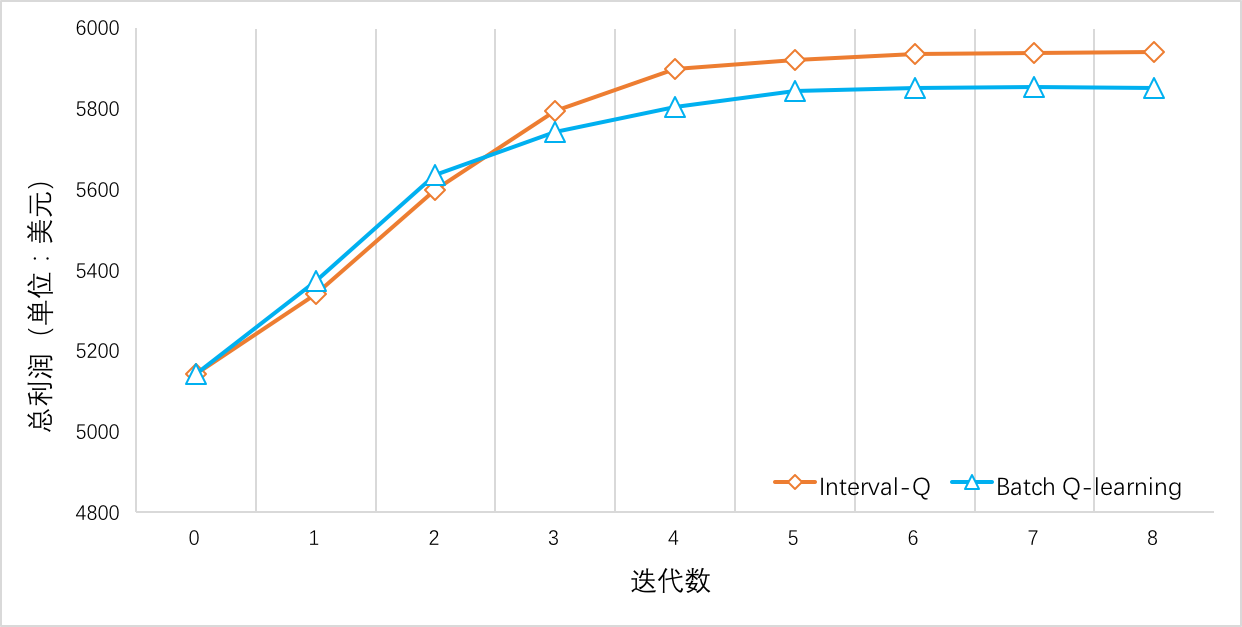
\includegraphics[width=1.0\textwidth]{e31}
\caption{Interval-Q算法和Batch Q-learning算法的总利润}
\label{fig:e31}
\end{figure}

\begin{figure}[htbp]
\centering
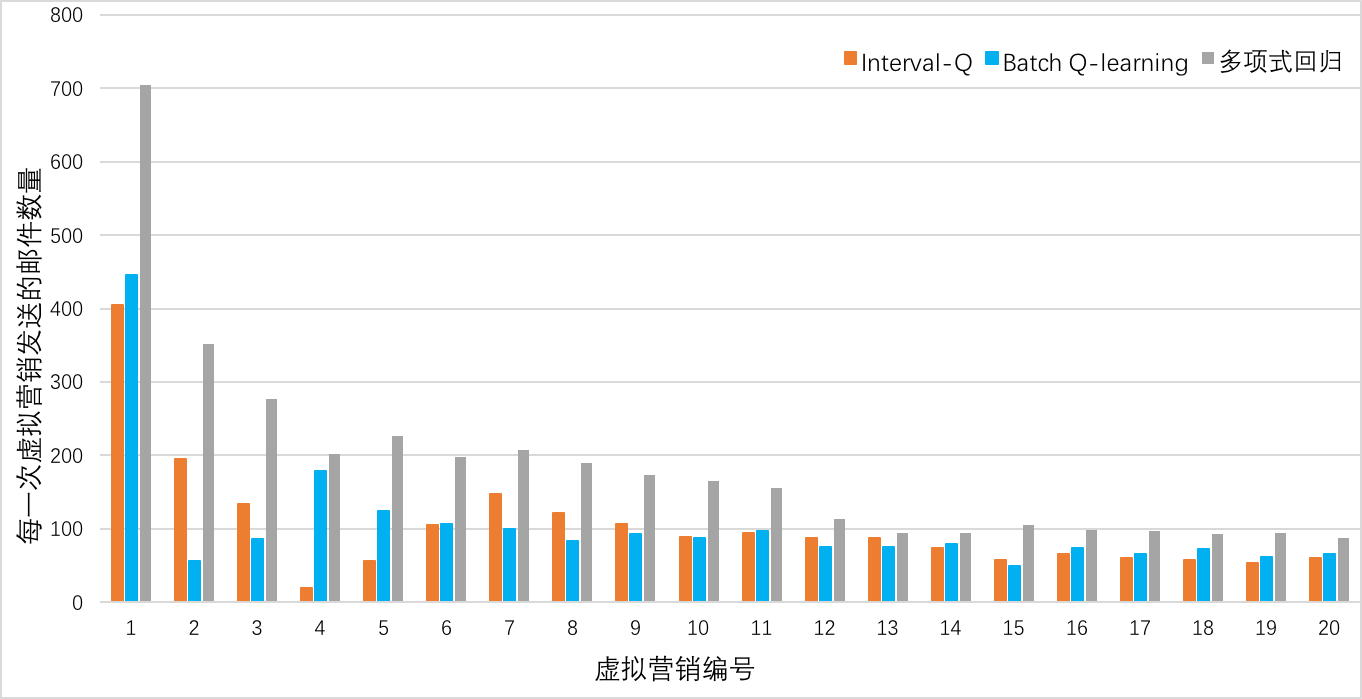
\includegraphics[width=1.0\textwidth]{e321}
\caption{每个虚拟营销发送邮件的数量}
\label{fig:e321}
\end{figure}

\paragraph{策略的变化}
上述长期利润是评价模型的策略质量最直观最重要的指标,但是为了分析监督学习方法和强化学习在输出策略上的变化情况,有必要考察一下以上三个模型在20次虚拟营销中发送邮件的数量以及每次虚拟营销所产生的利润值。另外,为了让试验的效果更加明显,在本实验,选择10000个募捐者进行评估测试,同样,每个模型进行5次实验,每次实验最大迭代次数为8,但是与第一部分实验不同的是每次实验的所使用的情节数据都是相同的。对于多项式回归模型,取5次试验中总收益最高的那个营销策略,对于Interval-Q、Batch Q-learning算法,取5次试验在第8轮迭代时总收益最高那个营销策略。按照这种方式得到三个营销策略,并将这三个策略在每次虚拟营销中发送的邮件数量以及产生的利润值记录下来,并分别绘制成柱状图,如图\ref{fig:e321}和\ref{fig:e322}所示。

\begin{figure}[htbp]
\centering
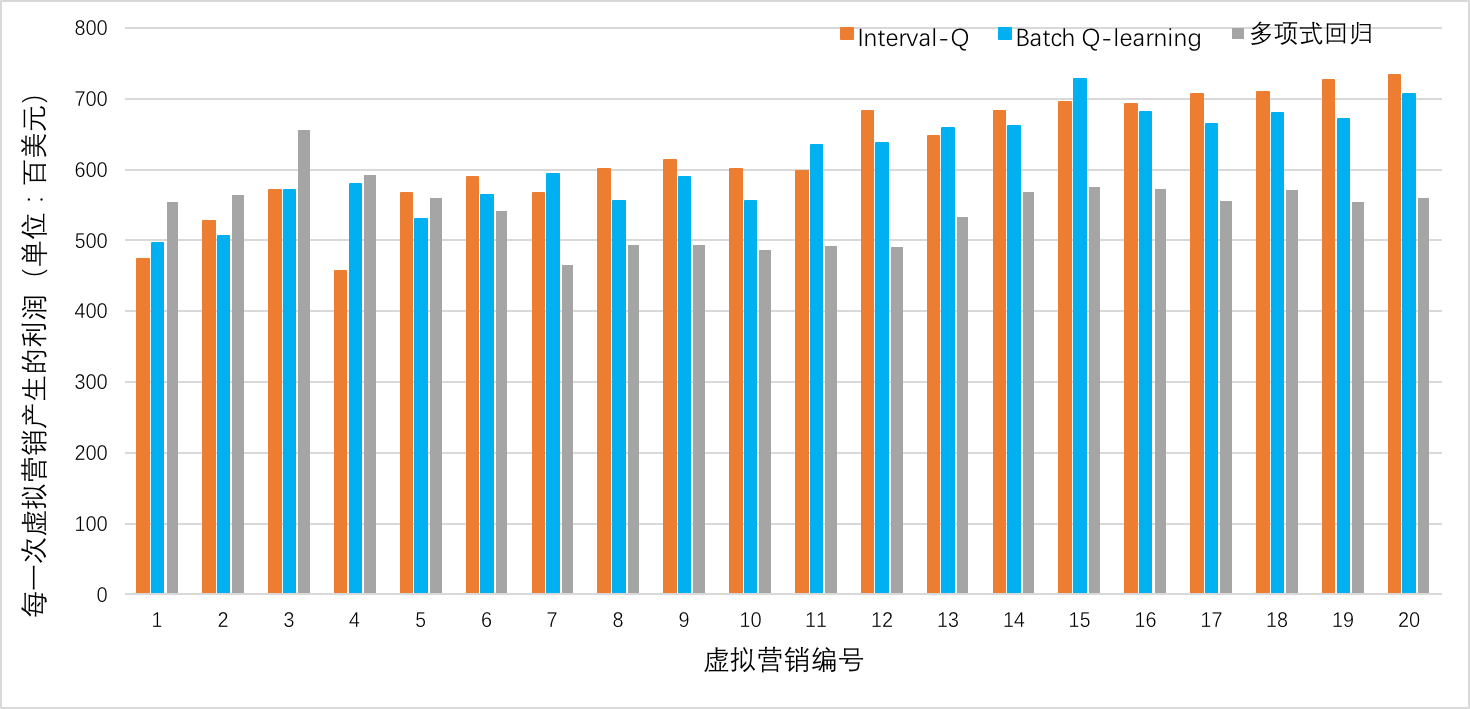
\includegraphics[width=1.0\textwidth]{e322}
\caption{每个虚拟营销中的总利润}
\label{fig:e322}
\end{figure}

首先,观察以上三个策略在20个虚拟营销过程中发送邮件的数量。从图\ref{fig:e321}中可以很明显地看出,Interval-Q和Batch Q-learning算法的营销策略在20个虚拟营销过程中所发送邮件的数量,远小于基于多项式回归算法的营销策略所发送邮件的数量。而Interval-Q算法的邮件数量(2070)比Batch Q-learning算法(2082)更少,从而说明Interval-Q算法有更好的成本控制能力。

% 但是,Interval-Q和Batch Q-learning算法在邮件发送数量上并没有多大区别。


接着,考察以上三个策略在20个虚拟营销过程中获得利润的变化情况。从图\ref{fig:e322}中可以看出,相比多项式回归方法,Interval-Q和Batch Q-learning算法在刚开始的几次虚拟营销中产生的利润比较低,但是在后续的营销中,其获得的利润在不断提升,这同样体现了强化学习方法在序贯决策问题中,因为考虑到了延迟影响并且以长期收益最大化作为学习目标,所以随着时间的推移,其产生的收益就会越来越高。而监督学习在学习中只考虑到了最大化即时收益,所以后续利润的增长就不是特别的明显。特别地,尽管Interval-Q和Batch Q-learning算法在20个虚拟营销中发送邮件的数量相似,但是Interval-Q算法所获得的总利润更高,特别是在最后的虚拟营销里,这主要归功于Interval-Q算法考虑到了时间间隔不固定的因素,因而可以更准确的进行值函数的逼近。

最后,结合图\ref{fig:e321}和图\ref{fig:e322}可以看出,尽管Interval-Q策略中第4次虚拟营销和Batch Q-learning策略中第5次虚拟营销,发送的邮件数量很少,但是仍然产生了很大的利润,而这个利润主要来源于之前营销活动的延迟反应。因为在该直邮营销的场景中,募捐者的延迟反馈会被记录到收到该反馈的那个日期里,而不是记录到发送该营销邮件的日期里,所以当在处理序列决策问题时,为了进行更有效的策略学习,应该考虑序列中的延迟影响,而这是监督学习方法很难办到的。另外,从图\ref{fig:e321}和图\ref{fig:e322}中可以看出,强化学习方法在制定营销策略的时候,是根据所采取的行为和收到的奖赏反馈来共同决定的。比如,在图\ref{fig:e321}中,Interval-Q算法在第3次发送邮件的数据相比第2次减少了,但是其产生的利润却增加了,所以在第4次制定营销策略的时候,Interval-Q算法就会有很大的概率选择继续减少邮件的数量,从图\ref{fig:e321}中也印证了这一点。

\begin{figure}[htbp]
\centering
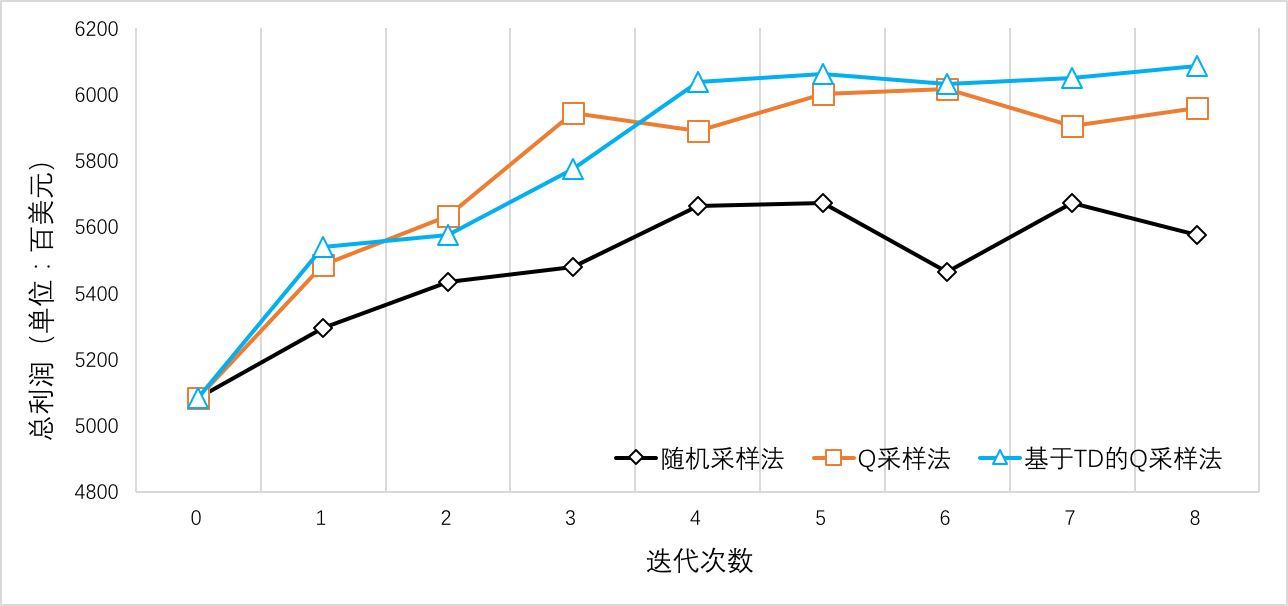
\includegraphics[width=1.0\textwidth]{e331}
\caption{不同采样方法下的利润}
\label{fig:e331}
\end{figure}

\begin{figure}[htbp]
\centering
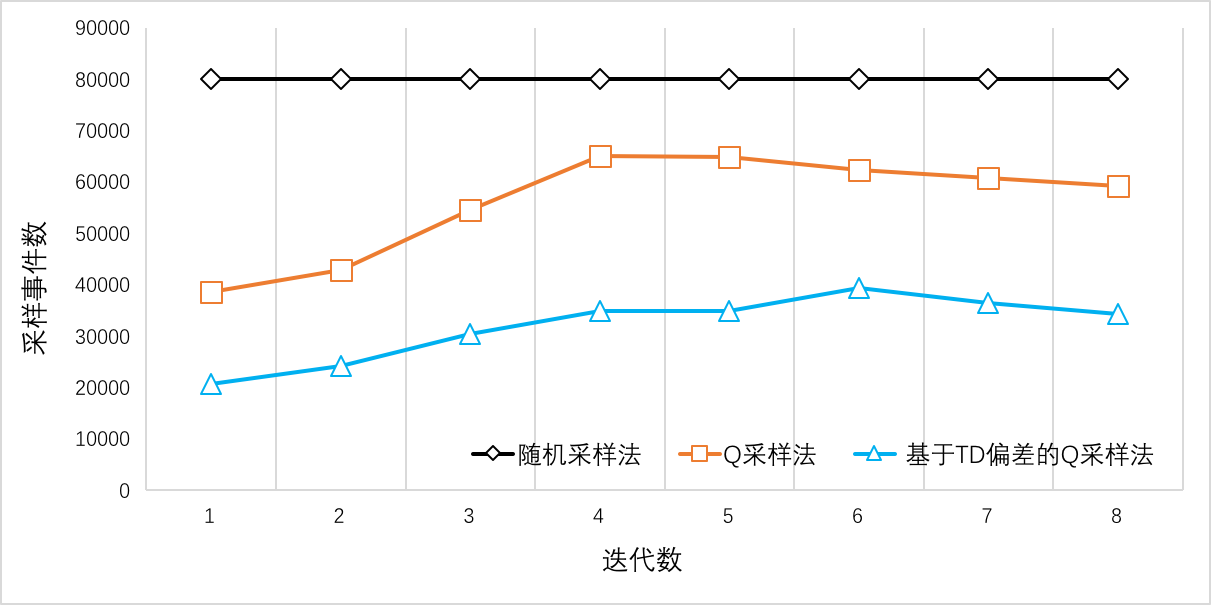
\includegraphics[width=1.0\textwidth]{e332}
\caption{不同采样方法下的采样数}
\label{fig:e332}
\end{figure}

\paragraph{采样方法比较}
最后,考察本文所提出的基于TD偏差的Q采样方法与Q采样法和随机采样法的效果对比,主要从采样数量和长期利润两个方面进行比较。在该实验中,选取一个规模大小为10000的情节集合,即160000个事件,在每轮迭代中随机抽取5000条情节(共80000个事件),然后再使用Q采样方法(算法:\ref{algo:SVR+Q_})和基于TD偏差的Q采样法(算法:\ref{algo:SVR+Q_2})进一步进行有条件采样。另外,在该实验中,基于TD偏差的Q采样法的阈值$\eta$设置为6.0。将每轮迭代所产生的利润平均值和所采样事件的数量记录下来,并绘制成图如\ref{fig:e331}和\ref{fig:e332}所示。

从图\ref{fig:e332}中可以看出,基于TD偏差的Q采样方法因为增加了TD偏差这一有效的约束条件,所以过滤掉了很多事件样本,其所采样的事件数量大约是Q采样方法的二分之一。不仅如此,从图\ref{fig:e331}可以看出,虽然基于TD偏差的Q采样方法采样数量下降了很多,但是其所获得的长期利润的能力却没有受到影响,甚至在最后几轮迭代的中,基于TD偏差的Q采样方法所产生的长期利润值超过了Q采样法。由此,可以得出,在面对数据规模比较大的现实应用中,基于TD偏差的Q采样法,在减少计算资源的情况也会学习到很好的策略。


\section{本章小结}
本章针对不定期直复营销场景中的营销时间间隔不固定,数据负载大导致学习速度慢的问题,基于传统的Q-learning算法进行改进。首先,给出直复营销在强化学习框架下的形式化描述以及基于Q-learning的算法模型,然后结合营销决策点间存在的时间间隔不固定问题,对Q-learning算法中值函数的更新方法进行改进,提出Interval-Q算法。接着,针对Interval-Q算法在处理大规模数据时的学习效率较低的问题,基于Q采样的方法,提出了基于TD偏差的Q采样方法。最后,介绍仿真环境的构建方法,并利用仿真环境从模型的长期收益、策略行为的变化以及采样方法的效果等三个方面对所提算法进行评估并对结果进行分析,评估结果验证了所提算法的有效性。

\cleardoublepage

\chapter{基于深度混合强化学习的直效营销策略}

\section{研究动机}
在马尔科夫决策过程中,要求系统的状态具有马尔科夫性,即下一个时刻$S_{t+1}$仅与当前的状态$S_{t}$和当前采取行为$A_{t}$有关,与之前拥有的状态和采取的行为都无关。所以,当采用强化学习对直复营销场景进行建模时,存在的一个假设是客户的当前状态完全概括了他与营销人员在此之前的整个交互历史。也就是说客户的下一步响应情况仅与他当前的状态和营销人员采取的下一步营销行为有关,与之前的交互历史无关。但是,和很多其他现实应用所面临的问题一样,在直复营销场景中,因为客户的状态存在部分可观测性(Partial Observability)的问题,使得上述这个假设很难得到满足。

在本文的第三章中,为了更好的捕捉募捐者的状态,在进行仿真实验的时候从观测数据中提取了大量募捐者特征,而这些特征有很多是需要借助专家的领域知识或经验才能获得的。即便如此,这也只概括了客户真实状态中的部分信息。因此,在对这些场景应用强化学习之前,进行状态的推断学习是很重要的。

在像直复营销这类复杂的现实场景中,构建这种具有马尔科夫性的状态是很难的。在强化学习的研究和应用中,处理部分可观测问题最常用的方法有两种,其一是使用部分可观测的马尔科夫决策过程(Partially Observable Markov  Decision Process,POMDP)\citep{kaelbling1998planning},其二是预测状态表示法(Predictive State Representation,PSR)\citep{littman2002predictive}。POMDP虽然有着坚实的理论基础,并且已经在一些诸如机器人、人机对话等领域取得了不错的表现\citep{pineau2003point,williams2007partially},但是POMDP模型的建立需要依赖部分可观测的名义状态(Nominal State),所以系统的POMDP是很难学习的,而且需要很多专家领域的先验知识来定义隐藏状态集和观测概率集。Littman等人于2002年提出了一种新的动态系统建模方法———PSR\citep{littman2002predictive},用于处理部分可观测的问题,他的优势在于仅通过观察值序列就可以预测未来事件。尽管PSR具有很强的表示能力,并且比POMDP方法更容易从数据中学到信息,但是仍然需要大量的领域知识来设计特征和核函数。

近年来,强化学习和深度神经网络的结合取得了重大突破,并成功的应用在了游戏、围棋等领域\citep{mnih2013playing, mnih2015human},形成了一个重要的研究方向,深度强化学习。深度强化学习的成功应用除了充分发挥强化学习技术在序贯决策上的优势外,还离不开神经网络的强大作用,其作用主要包括两点。一方面利用了神经网络强大的非线性逼近能力进行值函数的逼近,更好的学习最优策略,另一方面神经网络也可以自动的进行隐状态的学习和表示,一定程度上解决状态的部分可观测问题。与上述POMDP和PSR方法不同,基于神经网络的方法可以在不依靠专家领域知识的情况下,对任何问题都可以给出隐状态的合理表示方法\citep{deng2014deep},从而解决了在实际应用中,当使用强化学习时需要人为设计隐状态的困扰

受此启发,本文针对直复营销场景中的用户状态部分可观测问题,提出使用深度强化学习方法进行解决。进一步地,从深度强化学习DQN模型出发,结合直复营销场景的时序特点,提出使用基于循环神经网络的DQN网络:DQN_RNN,另外,为了更好的学习隐藏状态的表示方法以及保证值函数逼近效果,提出了基于RNN的深度混合强化学习模型,并对网络结构进行进一步的分析和优化。

\begin{algorithm}[htbp]
 \small
 \SetAlgoLined
 \SetKwRepeat{Repeat}{repeat}{until} 
 初始化回放记忆库$D$,记忆库大小为$N$\;
 利用随机参数$\bm{\theta}$初始化Q值函数\;
 初始化Q目标值网络$\bm{\theta}^{-}$,令$\bm{\theta}^{-}=\bm{\theta}$\;
 \For((循环每个情节)){$episode=1,\cdots, M$}{
	初始化情节(episode)的第一个状态:$S_{1}$\;
	% ,通过预处理得到该状态对应的特征输入:$\phi_{1}=\phi(s_{1})$\;
	\For((初始化情节中的每一步)){$t=1,\cdots, T$}{
		以概率$\epsilon$选一个随机行为$A_{t}$\;
		如果以上小概率事件没有发生,则选择当前值函数最大的那个行为:$A_{t}=\argmax_{a}Q(S_{t},a;\bm{\theta})$\;
		在仿真器中执行行为$A_{t}$,可以得到奖赏$R_{t}$以及环境的下一步状态$S_{t+1}$\;
		% 设置$s_{t+1}=s_{t},a_{t},x_{t+1}$,预处理得到对应的特征输入:$\phi_{t+1}=\phi(s_{t+1})$\;
		将转换样本$<S_{t}, A_{t}, R_{t}, S_{t+1}>$放到回放记忆库$D$中\;
		从回放记忆库$D$中均匀随机采样一小批转换样本$<S_{j}, A_{j}, R_{j}, S_{j+1}>$\;
		判断是否是一个情节的终止状态,若是,则Q目标值为$R_{j}$,否则利用Q目标网络$\bm{\theta}^{-}$计算Q目标$R_{j}+\gamma \max_{a^{'}}Q(X_{j+1},a^{'};\bm{\theta}^{-})$\;
		使用随机梯度下降(公式$\eqref{dituxiajiangq}$)更新当前网络参数:
		更新Q值函数当前网络(MainNet)参数:$\bm{\theta}=\bm{\theta}+\triangle \bm{\theta}$\;
		每隔$C$步更新一次Q目标网络(Target)参数;即:$\bm{\theta}^{-}=\bm{\theta}$\;
	}
 }
 % 输出最终策略:$\pi(s)=\argmax_{a}Q(s,a)$\;
 \caption{DQN算法}
 \label{algo:algorithm_DQN}
 \end{algorithm}


\section{DQN_RNN模型}

\subsection{DQN模型}
 DQN算法是在Q-learning算法($\ref{algo:algorithm_2}$)的基础上改进而来,如第二章所述,主要包括以下三个方面进行改进:

 1)使用卷积神经网络进行Q值函数的逼近。2)通过经验回放(Experience Replay)机制来解决强化学习中相关性以及非静态分布的问题。3)通过独立设置目标网络(Target Net)来单独处理时间差分算法中的TD偏差,进一步降低数据之间的关联性,从而削弱收敛不稳定的问题。

\paragraph{DQN模型流程}
 从文献\citep{mnih2015human}中可以得到DQN算法的伪代码如$\ref{algo:algorithm_DQN}$所示。进一步的,可以总结出DQN算法学习过程主要包括以下几步(DQN的算法流程图如图$\ref{fig:liuchengtu_DQN}$所示):

 \begin{figure}[htbp]
\centering
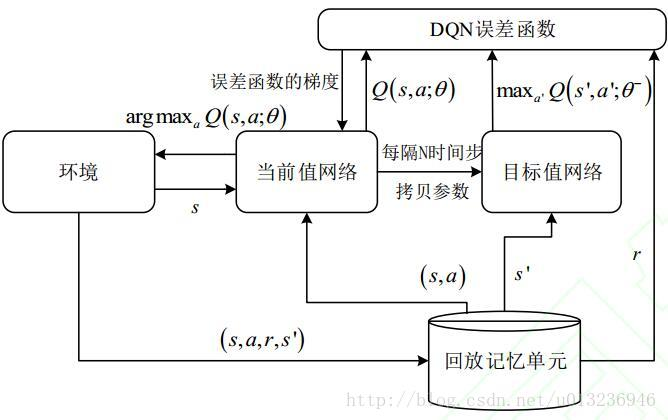
\includegraphics[width=0.9\textwidth]{liuchengtu_DQN}
\caption{DQN流程图}
\label{fig:liuchengtu_DQN}
\end{figure}
 

(1)构建回放记忆单元。在每个情节中,首先初始化第一个状态$S_{1}$,然后,在接下来的每个时间步里,按照$\epsilon-greedy$策略选择行为$A_{t}$,并在仿真器中执行$A_{t}$,即可得到对应的即时奖赏$R_{t}$和下一步的状态$S_{t+1}$,将此转换样本$<S_{t}, A_{t}, R_{t}, S_{t+1}>$放到回放记忆单元中。

(2)值函数的学习。从回放记忆单元中随机选取一小批转移样本,并分别使用当前值网络(MainNet)和目标值网络(TargetNet)计算出Q估计值 $Q(s,a;\bm{\theta})$和Q目标值$r+\gamma \max_{a^{'}}Q(s^{'},a^{'};\bm{\theta}^{-})$,然后得到损失函数$L=[r+\gamma \max_{a^{'}}Q(s^{'},a^{'};\bm{\theta}^{-})-Q(s,a;\bm{\theta})]^{2}$,并使用随机梯度下降法进行求解,以更新当前值网络MainNet的参数。
% $<S_{j}, A_{j}, R_{j}, S_{j+1}>_{j=1}^{N}$

(3)更新目标网络参数。经过若干步的训练后,将当前网络的参数拷贝给目标网络,进行目标网络的参数更新。 

(4)当DQN网络训练完毕后,将环境的当前状态$S_{t}$输入到当前值网络,便会输出DQN的动作选择策略$A_{t}=\argmax_{a}Q(S_{t},a;\bm{\theta})$。

\paragraph{DQN模型误差更新}
进一步地,DQN模型的损失函数构建过程参见图$\ref{fig:loss_DQN}$,从图中可以看出,当前值网络(MainNet)和目标值网络(TargetNet)都是关于状态$s$的网络。在进行损失函数的计算时,将状态$S_{t}$输入当前值网络,并根据行为$A_{t}$从当前值网络找到当前的Q估计值,然后将状态$S_{t+1}$带入目标值网络,得出Q目标值,Q目标值和Q估计值的均方误差即为当前的损失。

% 在DQN中增强学习Q-Learning算法和深度学习的SGD训练是同步进行的
\begin{figure}[htbp]
\centering
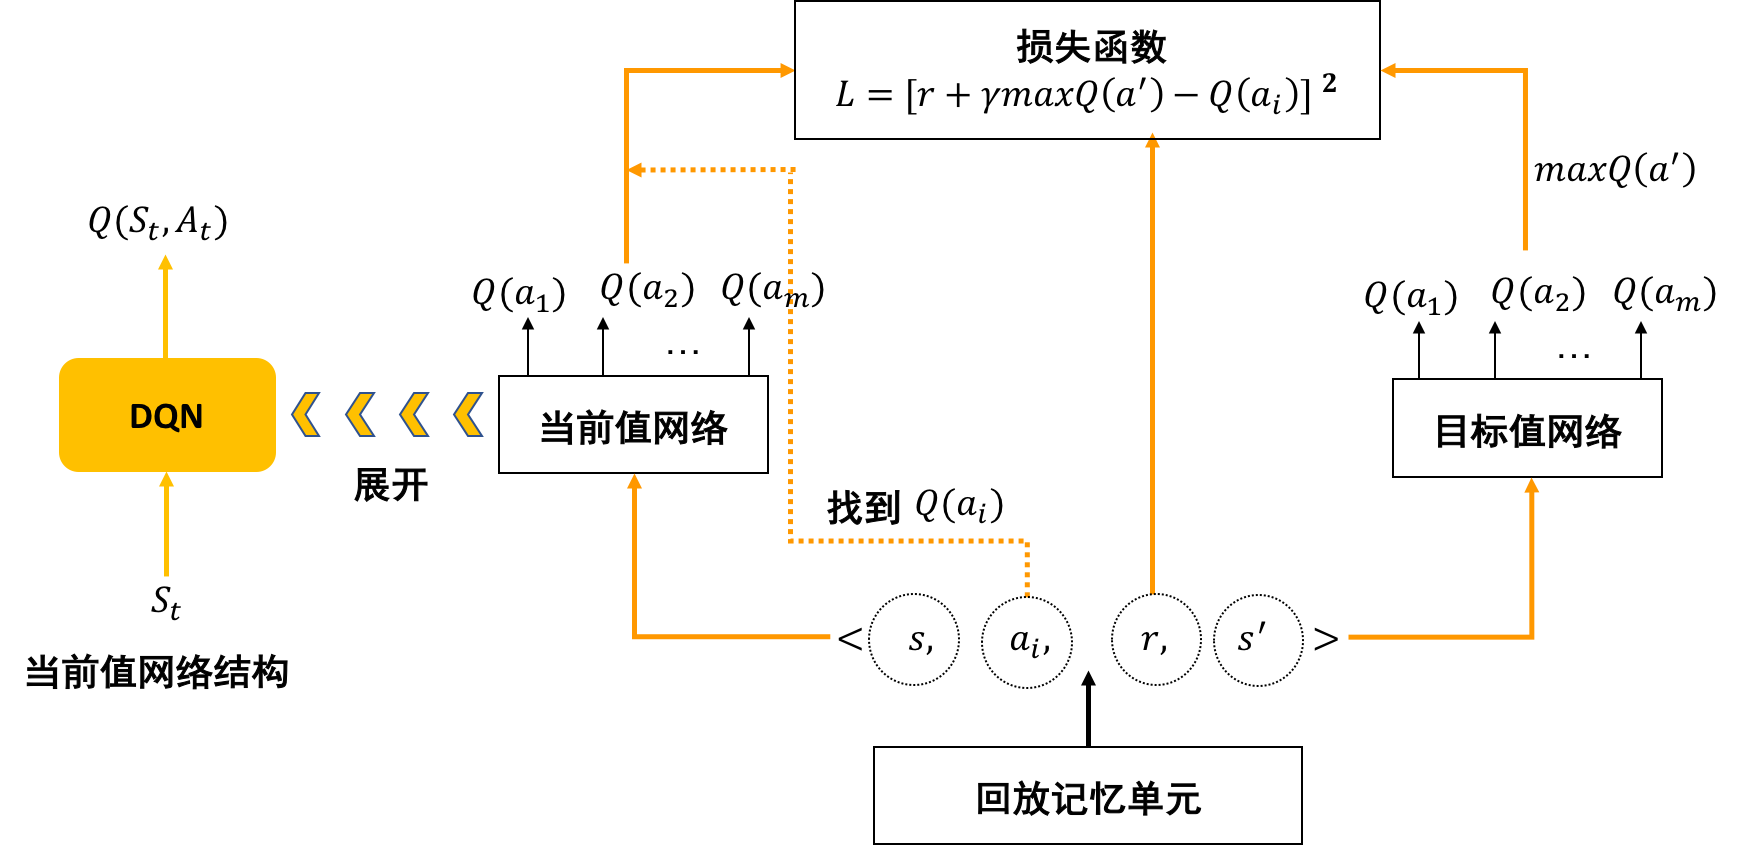
\includegraphics[width=0.6\textwidth]{loss_DQN}
\caption{DQN损失函数构造}
\label{fig:loss_DQN}
\end{figure}

\paragraph{DQN基准模型}
可以直接将DQN模型用于直效营销的场景的建模中。具体做法就是将客户的观测值$O_{t}$当作状态$S_{t}$,客户产生的利润当作即时奖赏$R_{t}$,营销人员采取不同类型营销方式作为行为$A_{t}$。在客户和营销人员的不断交互中形成转移样本$\{<O_{t}, A_{t}, R_{t}, O_{t+1}>\}_{t=1,2,\cdots}$,再按照上述DQN算法$\ref{algo:algorithm_DQN}$去训练网络的参数。经过若干次的训练后,当得到一个近似最优的Q值函数时,带入客户的状态,就可以按照贪婪的方式从值函数中选择最佳的营销行为$\argmax_{a}Q(s,a)$。

图$\ref{fig:dqn_crm}$为DQN当前值网络简化的网络示意图。其中,$O_{t}$为用户的观测值,$Q(S_{t},A_{t})$为在$t$时刻时,执行行为$A_{t}$所的到的Q估计值。需要注意的是,在使用DQN模型进行训练时,前一个输入和后一个输入之间是没有关系的。
\begin{figure}[htbp]
\centering
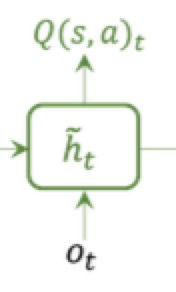
\includegraphics[width=0.2\textwidth]{dqn_crm}
\caption{DQN当前值网络结构}
\label{fig:dqn_crm}
\end{figure}

\subsection{基于RNN的DQN模型}
在将DQN模型应用到Atari游戏中时\citep{mnih2013playing},DeepMind团队之所以会选择卷积神经网络CNN作为Q函数逼近器,是因为在CNN结构中,通过卷积操作和池化操作可以大幅度降低网络参数,从而加快网络的训练。此外,CNN网络还非常善于抽取位置不变的特征,特别适合图像这类网格型结构的数据,因此广泛应用在图像识别领域。在视频游戏中,由于输入是图像,所以使用CNN结构的神经网络逼近值函数的效果就会很好。

但是,在CNN网络中假设输入是一个独立的没有上下文联系的单位,即前一个输入和后一个输入是没有关系的,所以CNN无法对时间序列上的变化进行建模。而样本出现的时间顺序对于自然语言处理、语音识别、手写体识别等应用非常重要。为了适应这种需求,就出现了另一种神经网络结构——循环神经网络(Recuurent Neural Network, RNN)

 \paragraph{RNN网络}
RNN是一种对序列数据建模的神经网络,可以连接先前的信息到当前的任务上来。具体的做法是:网络会对前面的信息进行记忆存储并应用于当前输出的计算中,即隐藏层之间的节点不再无连接而是有连接的,并且隐藏层的输入不仅包括输入层的输出还包括上一时刻隐藏层的输出。图$\ref{fig:rnn}$是一个RNN模型的简化结构展开图。
\begin{figure}[htbp]
\centering
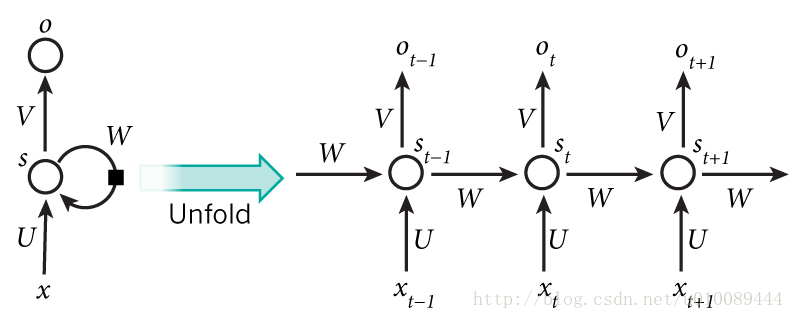
\includegraphics[width=0.8\textwidth]{rnn}
\caption{RNN模型的简化结构展开图}
\label{fig:rnn}
\end{figure}

在图$\ref{fig:rnn}$中,$x_{t}$表示$t$时刻的输入;$s_{t}$表示$t$时刻的隐藏层的记忆值(Memory),它基于上一时刻的隐状态和当前输入得到;
% \begin{equation}
% \begin{aligned}
% s_t=f(U x_{t}+W s_{t-1})
% \end{aligned}
% \end{equation}
% 其中,$f(\cdot)$一般是非线性的激活函数;
% 在计算$s_{0}$时,即第一个单词的隐藏层状态,需要用到$s_{−1}$,但是其并不存在,在实现中一般置为0。
$o_{t}$表示$t$时刻的输出。$U$是输入层到隐藏层的权重矩阵,$V$是隐藏层到输出层的权重矩阵,权重矩阵$W$就是隐藏层上一次的值作为这一次的输入的权重。需要注意的是:在传统神经网络中,每一个网络层的参数是不共享的,而在RNN中,所有层次均共享同样的参数,
% 其反应出RNN中的每一步都在做相同的事,只是输入不同,
因此大大地降低了网络中需要学习的参数。网络在$t$时刻接收到输入$x_{t}$之后,隐藏层的值是$s_{t}$,输出的值是$o_{t}$。
% 特别的,$o_{t}$的值不仅仅取决于$x_{t}$,还取决于$o_{t-1}$。
我们可以用下面的公式来表示循环神经网络的计算方法:
\begin{equation}
\label{rnn_1}
\begin{aligned}
o_{t}=g(V s_{t})
\end{aligned}
\end{equation}
\begin{equation}
\label{rnn_2}
\begin{aligned}
s_{t}=f(U x_{t}+W s_{t-1})
\end{aligned}
\end{equation}

式\eqref{rnn_1}是输出层的计算公式,输出层是一个全连接层,也就是它的每个节点都和隐藏层的每个节点相连。$V$是输出层的权重矩阵,$g$是激活函数。式\eqref{rnn_2}是隐藏层的计算公式,它是循环层。$U$是输入$x$的权重矩阵,$W$是上一次的值作为这一次的输入的权重矩阵,$f$是激活函数。从上面的公式我们可以看出,循环层和全连接层的区别就是循环层多了一个权重矩阵$W$。如果反复把式$\eqref{rnn_2}$带入到式$\eqref{rnn_1}$,我们将得到:
\begin{equation}
\label{rnn_3}
\begin{aligned}
o_{t}&=g(V s_{t})\\
&=V f(U x_{t}+W s_{t-1})\\
&=V f(U x_{t}+W f(U x_{t-1}+W s_{t-2}))\\
&=V f(U x_{t}+W f(U x_{t-1}+W f(U x_{t-2}+W f(U x_{t-3}+\cdots)))\\
\end{aligned}
\end{equation}

从式\eqref{rnn_3}可以看出,循环神经网络的输出值$o_{t}$,是受前面历次输入值$x_{t}$、$x_{t-1}$、$x_{t-2}$、$x_{t-3}$、$\cdots$影响的,这就是为什么循环神经网络可以往前看任意多个输入值的原因,也是它为什么善于按序列对单元进行建模的原因。

RNN的训练方法是采用基于时间的反向传播算法(BackPropagation Through Time, BPTT),具体的更新方法和BP更新方法相同。
% 但是,在处理较长序列的时候, RNN不能得到较好的性能。一个主要原因是,RNN在训练中如果向前考虑的很远的时候,会导致对应的误差项的值增长或者缩小的非常快,就会很容易发生梯度爆照或者梯度消失的现象,这导致训练时梯度不能在较长序列中一直传递下去,从而使RNN无法捕捉到长时间距离的信息。由此,提出了长短时记忆网络(Long  Short-Term Memory,LSTM)。

% 因为原始RNN的隐藏层只有一个状态,它对于短期的输入非常敏感,LSTM在此基础上增加了一个状态,让它保存长期的状态,从而解决了传统RNN无法处理长距离依赖的问题。新增加的状态称为单元状态(Cell State)。因为篇幅的限制,关于LSTM的原理在此不表,详见文献\citep{hochreiter1997long}。
 \paragraph{DQN_RNN}
 因为RNN网络在时序变化问题中的强大建模能力,为了更好的将强化学习应用在序列相关问题中,所以,出现了很多对基于RNN网络的DQN模型的研究\citep{hausknecht2015deep,narasimhan2015language}。在这些研究中,作者普遍采用的做法是,将DQN模型中的CNN网络替换成了RNN网络,希望通过对数据序列中存在长时依赖性的奖赏信息进行建模,来更好的处理状态部分可观测的问题\citep{bakker2002reinforcement,hausknecht2015deep,lin1993reinforcement,narasimhan2015language},以达到更好的函数逼近效果。经过实验发现,在文本、语音等序列相关问题上确实取得了比传统基于CNN网络的DQN模型更好的表现。

 同样地,在直复营销场景中,客户和营销人员的交互也是一个随时间而不断发生变化的过程。因此,如果使用基于RNN的DQN模型(记作DQN_RNN)对直复营销场景进行建模,可以充分利用RNN的长时依赖性更好的学习客户的状态表示方法,进而达到更好的策略学习的目的。

 结合文献\citep{hausknecht2015deep,narasimhan2015language}所设计的模型,可以得到DQN_RNN当前值网络的简化结构示意图$\ref{fig:rl_rnn}$。对应到直复营销场景中,$O_{t}$表示$t$时刻客户的观测信息,$\tilde{h}_{t}$为$t$时刻客户的隐状态信息,$Q(S_{t}, A_{t})$表示在$t$时刻,当状态$S_{t}$等于$\tilde{h}_{t}$且采取行为$A_{t}$时的Q估计值。因为隐状态$\tilde{h}_{t}$是关于上一时刻隐状态$\tilde{h}_{t-1}$和当前观测$O_{t}$的函数,所以,Q网络也是关于当前观测$O_{t}$和上一时刻隐状态表示方法$\tilde{h}_{t-1}$的函数。当Q值网络训练完毕后,以贪婪的方式选择最优的行为。

 \begin{figure}[htbp]
 \centering
 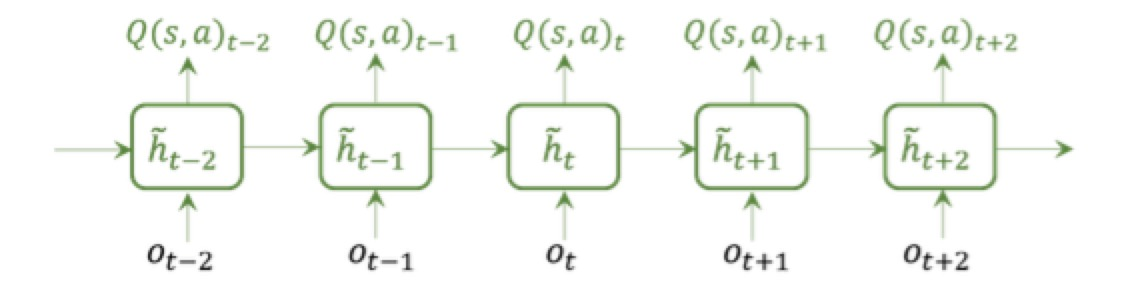
\includegraphics[width=1.0\textwidth]{rl_rnn}
 \caption{DQN_RNN当前值网络结构}
 \label{fig:rl_rnn}
 \end{figure}

 另外,与DQN模型的流程图$\ref{fig:liuchengtu_DQN}$相比,DQN\_RNN模型的流程图的当前值网络和目标值网络变成了RNN网络,并且回放记忆单元中存储的是有固定步长的序列,而不是独立的状态转移样本。在构建回放记忆单元时,需要模型和环境持续的进行固定步长的交互来形成一个序列样本。同样,从回放记忆单元中抽取批样本时,也是以序列样本的形式抽取,其他部分和图$\ref{fig:liuchengtu_DQN}$相同。损失函数的构造和DQN模型的损失函数构造方式($\ref{fig:loss_DQN}$)相同。

\section{基于RNN的深度强化学习混合模型}
在上述DQN\_RNN的模型中,利用RNN网络的长时依赖性,希望可以在时间变化的序列问题上更好的捕捉到状态的隐藏信息,进而在学习的过程更好的逼近Q值函数。所以,在RNN网络的优化过程中同时肩负着两个任务:

(1)Q值函数的逼近(策略学习)

(2)序列的长时依赖性学习(隐状态表示方法的学习)。

而对于只有一个RNN网络的DQN模型来说,同时进行这两个任务,往往会在实际的应用中导致学习效果不佳。在本节中,针对以上问题,提出了基于两个神经网络的混合强化学习模型。另外,根据训练方式的不同,又分为RNN+DQN$^{*}$两网络独立模型、1-RNN+DQN一步混合模型和2-RNN+DQN两步混合模型。

\subsection{两网络独立模型}
如上文所述,对于只有一个RNN循环神经网络的DQN\_RNN模型来说,在网络优化的过程中,同时兼具序列的长时依赖性学习和长期最大化策略的学习是比较困难的。那么,一个很自然的想法是,使用两个网络对以上两个任务分别进行学习,由此得到两网络独立模型。

本文的想法是:使用RNN和DQN两个网络进行训练。具体地,首先,进行RNN网络的训练:利用在交互过程中产生的监督数据,比如即刻奖赏、观测值等信息,通过RNN网络来对序列的长期依赖性进行建模,以单独的学习隐藏状态的表示方法。待RNN网络学习完毕后,进入DQN网络的训练:将观测值输入到学好的RNN网络,再将RNN网络学习到了隐状态信息作为DQN网络的输入状态,然后依靠DQN网络强大的非线性表达能力逼近Q值函数,以进行更充分的策略学习,达到最大化累积奖赏的目的。

其中,第一个部分属于监督学习过程,可以充分发挥RNN网络对时间序列建模的优势,第二个部分属于强化学习过程,可以充分发挥DQN网络对值函数学习的优势,通过这两个网络的优势互补,可以进行更有效的强化学习。将此模型记作:RNN+DQN$^{*}$

两网络独立模型的结构图如图$\ref{fig:rnn+dqn}$所示。左边部分为RNN网络的监督学习过程,其中,$O_{t}$是观测值,$h_{t}$是藏状态信息,$O_{t+1}^{'}$是$t+1$ 时刻的预测的观测值,$R_{t}$。右边为DQN网络的强化学习过程,其中,$O_{t}$是观测值,$h_{t}$是藏状态信息,$Q(S_{t},A_{t})$是$t$时刻Q的估计值,它是一个关于隐状态$h_{t}$的函数。

在测试阶段,将上一时刻的隐状态信息和这一时刻的观测值作为RNN的输入,然后再将产生的隐状态信息输入到已经学习好的Q值网络中,以贪婪的方式选择最优的行为。

同样,RNN+DQN$^{*}$的误差构造也分为两个部分,如图$\ref{fig:rnn+dqn}$所示。左边为RNN监督学习的误差构造过程,主要是利用预测的下一步观测值和预测的奖赏值与真实的下一步观测值和奖赏值来构造损失函数训练RNN网络。右边为DQN网络的误差构造过程,虽然都是和之前DQN网络的误差构造方法相同,都是利用Q目标值和Q估计值的均方误差作为损失函数,但是两个网络的输入从观测值变成了RNN的隐状态值。

\begin{figure}[htbp]
\centering
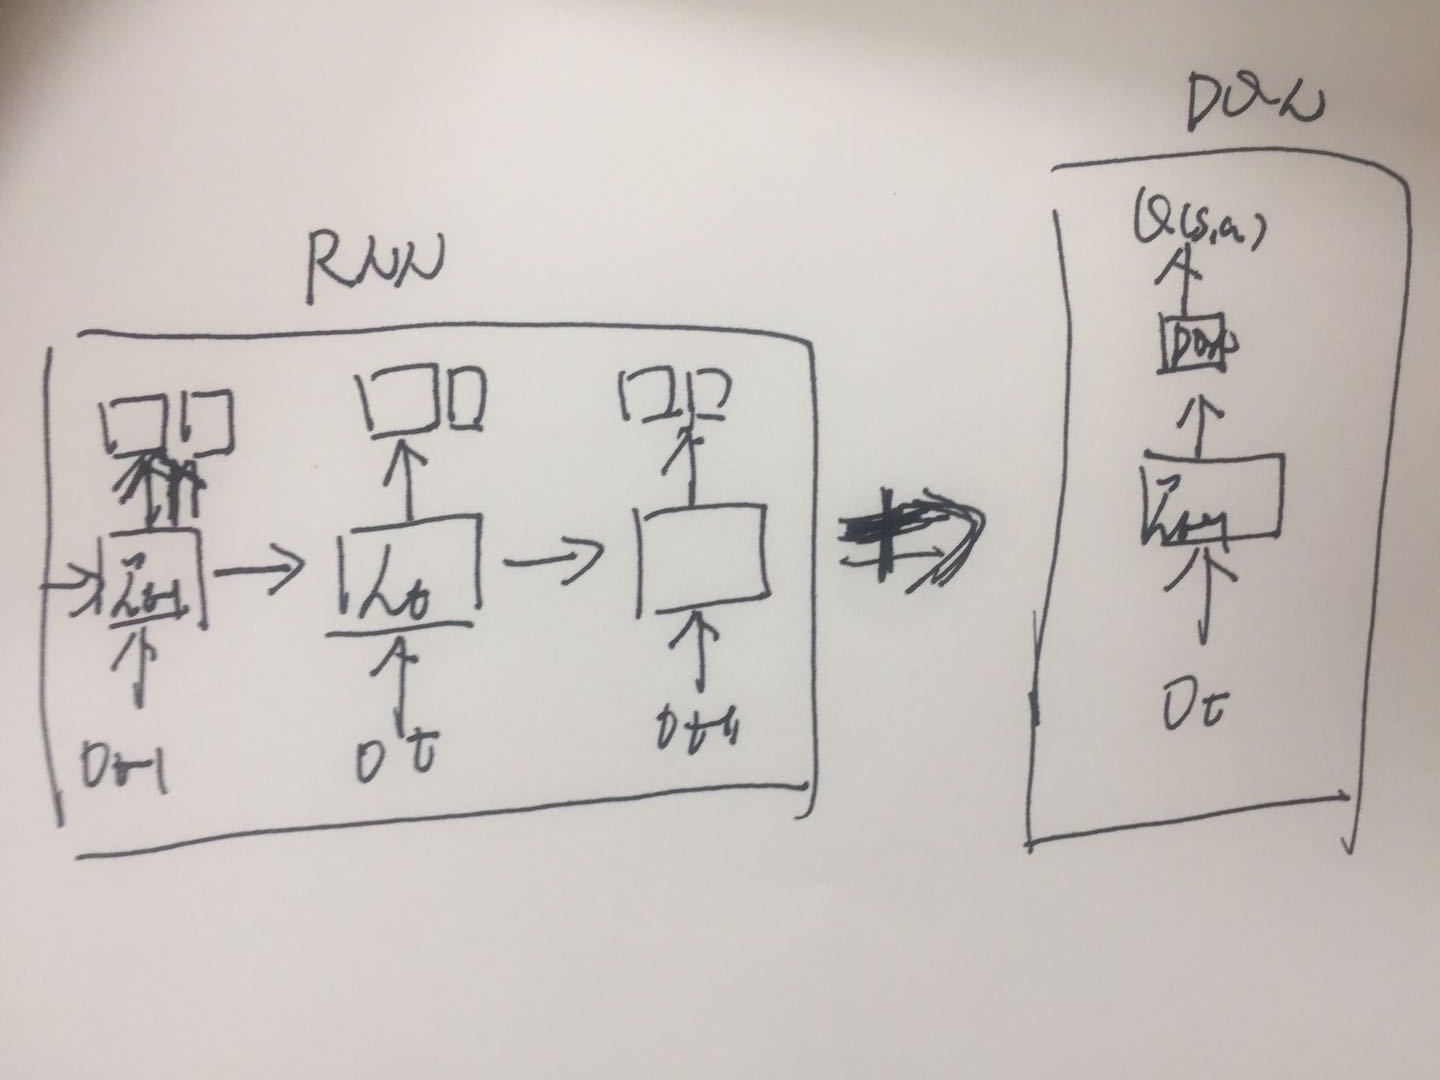
\includegraphics[width=0.8\textwidth]{rnn+dqn}
\caption{RNN+DQN$^{*}$网络结构图}
\label{fig:rnn+dqn}
\end{figure}

\subsection{一步混合模型}
在RNN+DQN$^{*}$模型中,虽然充分利用了RNN网络和DQN网络各自的优点,但是仍然存在一个问题:两个网络的优化过程被完全割裂开来,这样造成的一个后果就是我们很难知道已经训练好的RNN网络是否可以让DQN网络学到好的Q值函数,或者说很难知道RNN网络训练到什么程度才可以让DQN更好的产生一个Q值函数。

基于这个想法,本节提出一种联合训练的方法。让RNN网络在每学到一个隐状态表示方法后,就立刻让DQN网络以此隐状态表示方法产生的输出作为状态输入进行学习,两个网络交替进行更新,直到DQN网络学到一个好的Q函数,就停止学习。将这种模型称为一步混合模型1-RNN+DQN。

1-RNN+DQN的网络结构如图$\ref{fig:rnn_dqn}$所示,其中,$O_{t}$是观测值,$h_{t}$是隐藏状态,$O_{t+1}^{'}$是预测的$t+1$时刻的观测值,$R_{t}$是预测的$t$时刻即时奖赏值,$Q(S_{t},A_{t})$是$t$时刻预测的Q值。蓝色部分对应着RNN网络的监督学习部分,红色部分对应着DQN的强化学习部分。同样地,DQN的输入是RNN模型的隐状态。只不过在参数优化的过程中,两个网络依次交替进行。

具体来说,在训练阶段,使用联合训练的方法。首先,在每一个时刻,通过预测下一步的观测值和即时奖赏值来训练RNN网络,然后将此时训练过程中产生的隐状态作为DQN网络的输入,再通过DQN网络来逼近学习Q值函数。以上这两个步骤在随机梯度的迭代过程中依此交替的进行。在测试阶段,与DQN\_RNN模型类似,将环境观测信息输入RNN网络,然后将RNN网络产生的隐藏信息作为输入状态导入到训练好的Q值网络中,以贪恋的方式选择最优行为。

特别需要强调的是,与文献\citep{hausknecht2015deep,narasimhan2015language}中所提出的模型不同的是,在训练的过程中,
使用监督信号来学习隐状态的信息,并且将监督学习的误差反向传播到RNN网络的头部,但是,强化学习的误差信号只反向传播到RNN网络的隐藏层,并不参加RNN的训练。如图$\ref{fig:rnn_dqn}$所示,1-RNN+DQN模型的误差构造过程和RNN+DQN$^{*}$的误差构造过程类似,只是没有没有分开进行,而是依次交替进行。

因为在1-RNN+DQN模型的学习过程中,RNN网络和DQN网络按照上述训练方法依次进行,期间没有发生网络结构的变化,因此我们称之为一步混合模型。
\begin{figure}[htbp]
\centering
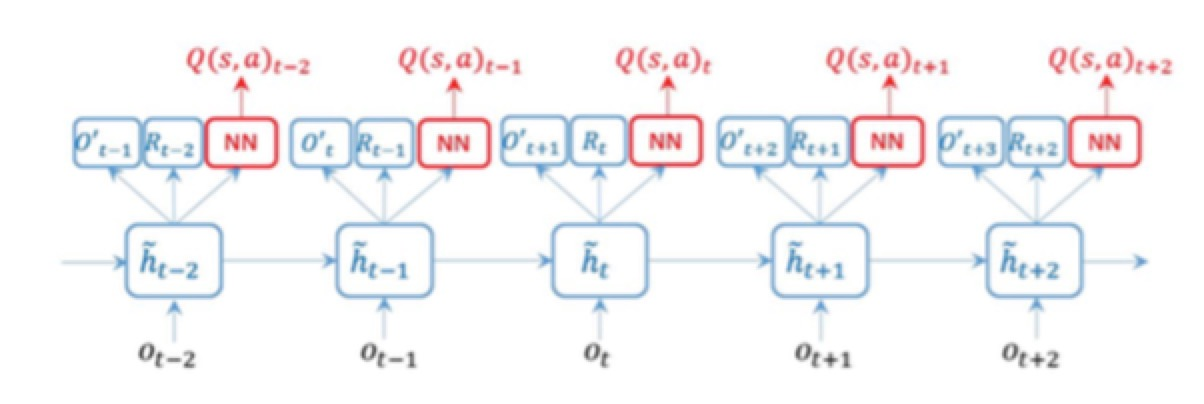
\includegraphics[width=1.0\textwidth]{rnn_dqn}
\caption{1-RNN+DQN模型结构图}
\label{fig:rnn_dqn}
\end{figure}

\subsection{两步混合模型}
在1-RNN+DQN模型中,通过使用联合训练的方法,我们可以更容易的为DQN网络的训练找到合适的RNN网络模型,以使得更好的逼近Q值函数。但是,从[图]中可以清晰的看出:在RNN网络训练的过程中,监督信号的误差传递到了RNN的头部,而在DQN网络的训练过程中,误差信号只传递到RNN的隐藏层。也就是说两个网络之间并没有进行误差的传递。这样会引起一个问题:

最初的目标是希望利用模型来学习关于观测值$o_{t}$的Q值函数,但是这种网络结构割裂了Q值函数和观测值之间的关系,导致我们在训练DQN网络的时候必须完全信任RNN网络关于隐状态的表达能力的,而无法直接接触到观测值。又因为针对RNN网络
% 的隐状态表达能力
的学习只用到了观测值和奖赏信息,并没有利用Q值信息。所以,在1-RNN+DQN模型训练的最后几个循环中,如果抛弃监督学习的过程,而将Q值的误差信息反向传播到RNN网络的头部,来同时更新RNN网络和DQN网络,进行参数的整体微调,就可以将观测值和Q值函数联系了到一起,期望会在一定程度上提升模型的效果。

所以,基于以上的想法,本节提出了两步混合模型,记为2-RNN+DQN。如图$\ref{fig:2-rnn-dqn}$所示,2-RNN+DQN模型在训练时共分为两个阶段,第一阶段,按照1-RNN+DQN的方法进行训练,学习到两个网络的参数向量$\bm{\theta}^{'}$和$\bm{\theta}^{''}$;第二阶段,将RNN网络的隐藏层和DQN网络的输入层连接起来,组成一个新的网络结构$[\bm{\theta}^{'},\bm{\theta}^{''}]$,新的网络的输入是观测值,输出是Q函数。通过这种方式,便可以在第二阶段将Q值函数的误差反向传播到RNN头部,来进行整体参数的微调。在测试阶段,将观测值输入到第二阶段新的网络结构中,通过贪婪的方式从Q值函数中选择最佳的行为。

% 训练时两个阶段训练时间应该如何把握。本实验采用的方法是将训练数据集按照8:2的比例分成两份,第一份用于第一阶段的训练,第二份用于第二阶段的训练。

\begin{figure}[htbp]
\centering
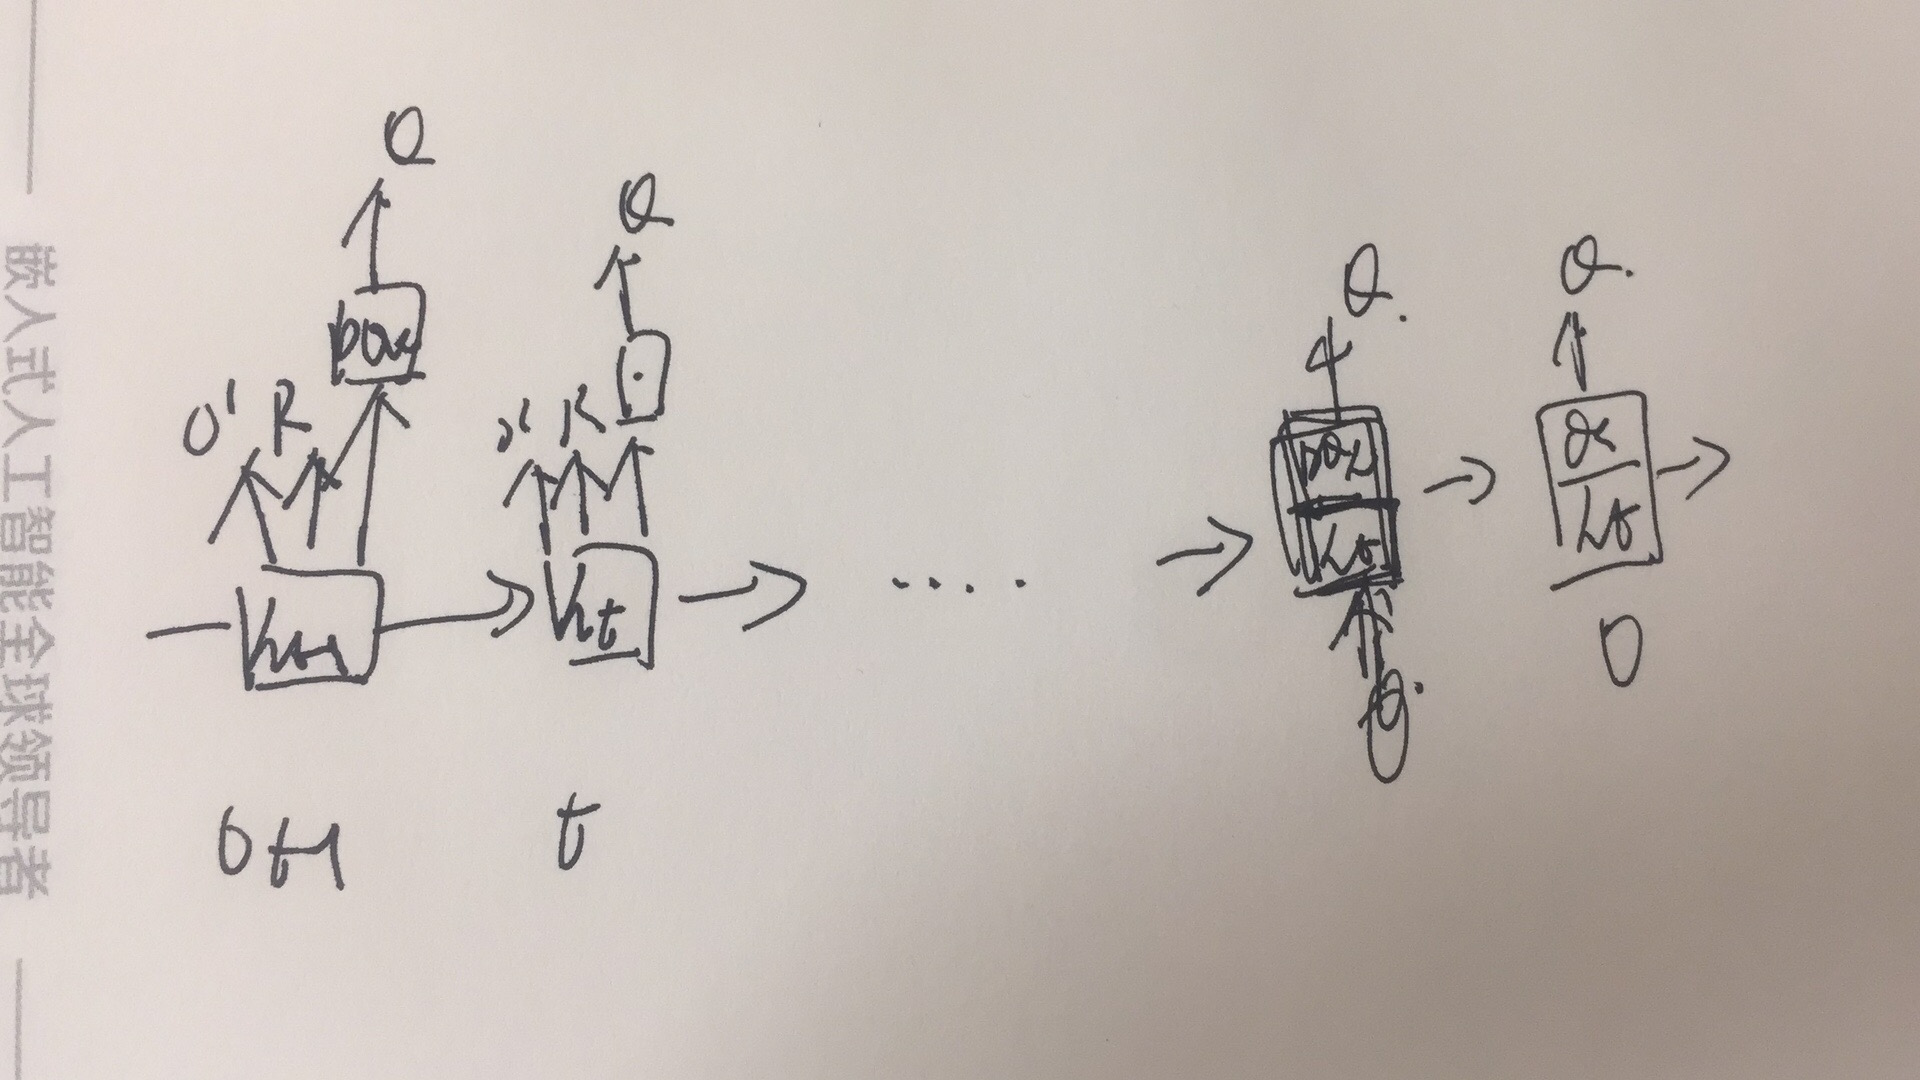
\includegraphics[width=1.0\textwidth]{2-rnn-dqn}
\caption{rnn-dqn框架}
\label{fig:2-rnn-dqn}
\end{figure}

\section{实验仿真}


\subsection{数据集}
本节,仍然选择使用UCI数据库中关于直邮营销著名的公开数据集KDD-CUP 1998\footnote{https://kdd.ics.uci.edu/databases/kddcup98/kddcup98.html}。但是,在数据特征的选择上,和第三章不同。

将原始数据集中每个募捐者的交互序列看成一个含有23步的时间序列,可表达为:$<O_{1},A_{1},R_{1},\cdots,O_{22},A_{22},R_{22},O_{23}>$,当使用CNN网络和DQN网络进行训练时,其输入为当前的观测值$O_{t}$,当涉及RNN网络的训练时,其输入为一个观测序列$<O_{1},O_{2},\cdots,O_{22},O_{23}>$
其中:

(1)$O_{t}$:表示每个募捐者的当前观测特征值。是从第三章的用户特征里取五维所组成的向量,如表~\ref{tab:obser_donors4}所示:
\begin{table}[htbp]
  \centering
  \caption{捐助者特征的选取}
  \label{tab:obser_donors4}
  \begin{tabular}{cl}
    \toprule
      特征 & 描述 \\
    \midrule
      age & 捐助者的年龄 \\
      income & 捐助者的收入 \\
      frequency & 该捐助者捐助的频率\\
      ramntall & 捐助的总金额 \\
      recency & 距离上次捐助的时间 \\
      % nrecproms & 之前六个月里,给该捐者者发送直邮营销的次数\\
      % nrecgifts & 之前六个月里,捐助者捐助的次数\\          	  
    \bottomrule
  \end{tabular}
\end{table}

(2)$A_{t}$:需要特别注意的是,本节的行为选取和第三章不同,因为在KDD-CUP 1998的数据库中,包含11种不同的邮件类型,所以可以当作11个不同的行为,加上一个不进行直邮营销这一行为,所以本章可选择的行为集合中一共有12个行为。所以,本章试验的目的就变成了,PVA采取什么样类型的邮寄行为,可以使的所获得的长期收益最大化。

(3)$R_{t}$:$R_{t}$表示执行行为$A_{t}$带来的奖赏,和第三章一样,使用PVA从捐助者获得的利润作为对应的奖赏信息。

\subsection{仿真环境}
\paragraph{仿真环境构造}
本章所构造的仿真环境和第三章仿真环境的构造原理大致相同。不同的是,预测每个捐助者响应概率的模型$P(s,a)$和产生奖赏信息的模型$A(s,a)$均使用的RNN网络来进行预测,期望通过RNN网络的长时依赖性来获得更准确的响应模型和获得的奖赏。

当有了模型$P(s,a)$和$A(s,a)$,我们可以使用如下过程来构建马尔科夫决策过程。

(1)给定状态$s$和行为$a$下的即时奖赏$R(s,a)$可以通过这两个模型得到:以$P(s,a)$的概率来掷一枚硬币,并以此来判断捐助者是否会产生反馈。即:出现正面的概率为$P(s,a)$表示捐助者会产生反馈,出现反面的概率为$1-P(s,a)$表示捐助者忽略掉了本次募捐邮件,不会产生任何反馈信息。如果没有出现反馈,那么捐助额为$0$,如果产生了反馈,那么用户的捐助金额为$A(s,a)$。即时奖赏$R(s,a)$等于捐助额减去邮寄的成本。

(2)状态转移方程也可以通过使用这两个模型计算每一个状态特征的变化情况而得到。比如:如果PVA采取的行动为1,numprom的值就会加1,否则保持不变;同样的,如果上述掷硬币的方式出现正面朝上,那么ngiftall的值就会加1,否则保持不变;有了这两个值(numprom,ngiftall),那么frequency的值也就可以计算出来了。类似的,其他状态特征也是通过这种方法计算的到的。

\paragraph{仿真评估方法}
有了上述马尔科夫决策过程的模型和状态转移方程,就可以使用如下的方式来构建我们的评估实验。

(1)首先,随机选择一定数量规模(5000)的捐助者,并设置他们的初始状态。本实验中将所选择的捐助者的初始状态设置为第7个营销活动时的状态。

(2)然后,使用学习好的强化学习模型输出策略:对每个捐助者是否应该采取营销行为。

(3)最后,使用模型$P(s,a)$和$A(s,a)$,可以得到预估的即时奖赏以及下一时刻的状态。记录这些得到信息,然后进入下一次的邮寄决策中。

就这样,按照上述的三个步骤,每循环一次就会模拟一次虚拟的直邮营销的过程。本节实验中,重复循环20次,就得到了20次的模拟直邮效果。

\subsection{仿真结果}

(1)长期收益

 首先比较以上六个模型在20次模拟直邮中的长期总收益,以下为六个模型的网络结构以及参数。
 
 \begin{table}[htbp]
  \centering
  \caption{网络结构参数}
  \label{tab:wangluojigoucanshu}
	% \begin{tabular}{p{0.9\columnwidth}} 
  \begin{tabular}{llp{10cm}}  
    \toprule
      序号 &模型 & 结构及参数描述 \\
    \midrule
      1 &RNN &一个输入层,一个隐藏层,一个输出层。其中:batch大小:512,隐藏层神经元个数:128 ,学习率:0.001\\
      2 &DQN & 两个卷积层,第一个卷积层(strides=1, patch = 2, padding='SAME', 卷积核:32)第二个卷积层(strides=2, patch = 2, padding='SAME', 卷积核:64),两个全联接层,激活函数:relu,学习率:0.001,batch大小:512\\
      3 &DQN_RNN &一个RNN网络,参数同1 \\
      4 &RNN+DQN$^{*}$ & 一个RNN网络,一个DQN网络,参数同上1,2\\
      5 &1-RNN+DQN & 一个RNN网络,一个DQN网络,参数同1,2\\
      6 &2-RNN+DQN & 一个RNN网络,一个DQN网络,参数同1,2 \\
      % nrecproms & 之前六个月里,给该捐者者发送直邮营销的次数\\
      % nrecgifts & 之前六个月里,捐助者捐助的次数\\          	  
    \bottomrule
  \end{tabular}
\end{table}

 从原始数据集中抽取10000个捐助者序列分别进行以上模型的训练,然后将抽取的样本按照1:4的比例分割成训练集和测试集。进行20波(epoch)的训练,并在每波训练完毕后,按照上述方法进行仿真试验,评估模型的质量,并记录每波模型输出策略的利润值。每组试验运行5次,并取这5次试验在每波中的平均值作为最终的结果。表[]展示上述六个模型在第20波输出策略的总收益。图[]展示了20波训练过程的模型训练情况,其中在2-RNN+DQN模型中,在最后五波中的后10个batch进行两步训练。

(2)不同数据的收据搜集方式

 为了考察不同数据搜集方式对模型试验结果的营销,本部分考虑利用仿真环境重新构建数据集。

 具体地,随机抽取10000个捐助者的序列数据,然后按照1:4的比例分割成训练集和测试集。取训练集中的捐助者的初始状态,然后从行为集合中随机的选取行为,并在仿真环境中执行,得到捐助者的下一状态和此时的奖赏信息。将次作为捐助者的第一时刻的交互数据,按照这种方式,重复进行23次,同样得到了8000个捐助者含有23个时间步的交互序列。

 然后按照上述的试验方法进行试验,同样5次的试验,每次试验20波,然后去最后一次试验最后一波策略的平均值作为最终各模型在次数据集下的策略结果。

 正确的探索对于学习良好的政策是必要的,从图[]中可以清楚的看到,采用随机选取策略的方式得到的收益明显大于按照pva给定的数据集训练所得的结果。这在一定程度上说明了,PVA的实际数据收集政策似乎是确定性的,同一步骤对所有捐助者采取同样的行动。因此,这个数据集很少或根本没有探索。 

 另外,从RNN和CNN网络输出的结果来看,因此强化学习算法比缺乏监督学习算法更容易受到缺乏探索的影响,因为强化学习在学习的过程中试图去预测将来会发生什么,探索的越少,对强化学习来说就会引入更多的误差,这与图[]所示的结果一致。

(3)不同训练规模

在最后一组实验中,通过改变了数据大小,看它是如何影响每个模型的性能的。从原始数据中随机的选取5000,10000,20000和50000个捐助者的信息分别进行试验。同样按照上述所示的方法进行训练,从表中可以清晰的看到随着数据量的提升,其结果并没有很大的变化,这说明了小数据集(5000条样本序列)同样足以产生高效的营销策略。


\section{本章小结}
本章为了解决直效营销的场景的客户生命周期最大化和状态部分可观测的问题,研究了基于RNN的深度强化学习混合模型。首先介绍场景特点,阐明本章采用基于RNN的深度强化学习的出发点,然后介绍通过介绍先有的DQN网络和DQN\_RNN网络,并分析其在解决此类问题中存在的学习能力不足的问题,提出了基于RNN的深度强化学习混合模型,并在此基础上根据网络结构的不同,提出了R两网络独立模型NN+DQN_RNN$^{*}$、一步混合模型1-RNN+DQN\_RNN和两步混合模型2-RNN+DQN\_RNN,加之之前介绍的三个基准模型DQN、RNN以及DQN_RNN,一共提到了针对直效营销场景的六种模型,第五章会对他们依次进行试验分析。
\chapter{结论}


\section{工作总结}

\section{工作展望}
 
\bibliography{bib/ustc}

\appendix


\backmatter
\begin{acknowledgements}

在研究学习期间,我有幸得到了三位老师的教导,
他们是:我的导师,中国科大XXX研究员,中科院X昆明动物所马老师以及美国犹他大学的XXX老师。
三位深厚的学术功底,严谨的工作态度和敏锐的科学洞察力使我受益良多。
衷心感谢他们多年来给予我的悉心教导和热情帮助。

感谢XXX老师在实验方面的指导以及教授的帮助。
科大的XXX同学和XXX同学参与了部分试验工作,在此深表谢意。

\end{acknowledgements}

\begin{publications}

\section*{已发表论文}

\begin{enumerate}
\item Wang X, \bm{\text{Li P}}, Wang L, et al. A novel genetic algorithm based on circles for larger-scale traveling salesman problem[C]//Robotics and Automation Sciences (ICRAS), 2017 International Conference on. IEEE, 2017: 189-194.
% \item A A A A A A A A A
% \item A A A A A A A A A
\end{enumerate}

\section*{待发表论文}

\begin{enumerate}
\item Wang X, \bm{\text{Li P}}, Ammar H, et al. A budget allocation algorithm for multi-channel marketing with Q-learning [C]//Pattern Recognition (ICPR), 2018 24rd International Conference on. IEEE.(已接收)
\item Wang X, \bm{\text{Li P}}, Ammar H, et al. A hybrid model of deep Reinforcement Learning for direct marketing [C] // Next Generation Data-driven Networks (NGDN), 2018 International Workshop on. IEEE.(已接收)
\end{enumerate}

\section*{参与的科研项目}
\begin{enumerate}
\item A A A A A A A A A
% \item A A A A A A A A A
% \item A A A A A A A A A
\end{enumerate}

\end{publications}


\end{document}

 %1、摘要中可以使用缩写吗?
 %2、第二章的英文需要首字母大写吗?
 %3、描述问题时:各个营销点的时间间隔不固定
     % 描述算法时:可变时间间隔问题
  % 4、第一章研究现状,回归?
    % 第一张的研究现状,需要写强化学习?研究热点部分是不是应该换个名字或者说法?

    % 第三章:标准化 归一化
           % 可变时间间隔














